%========= File containing the main LaTex document ========%
%                                                          %
% Copyright (C) ISI - All Rights Reserved                  %
% Proprietary                                              %
% Written by Med Hossam <med.hossam@gmail.com>, April 2016 %
%                                                          %
% @author: HEDHILI Med Houssemeddine                       %
% @linkedin: http://tn.linkedin.com/in/medhossam           %
%==========================================================%

%\documentclass[pfe]{./tpl/isipfe}
\documentclass[]{./tpl/isipfe}
\graphicspath{{./img/}}

%\usepackage{hyperref}


%=========== File containing some new commands ============%
%                                                          %
% Copyright (C) ISI - All Rights Reserved                  %
% Proprietary                                              %
% Written by Med Hossam <med.hossam@gmail.com>, April 2016 %
%                                                          %
% @author: HEDHILI Med Houssemeddine                       %
% @linkedin: http://tn.linkedin.com/in/medhossam           %
%==========================================================%

\newenvironment{changemargin}[2]{%
\begin{list}{}{%
\setlength{\leftmargin}{#1}%
\setlength{\rightmargin}{#2}%
}%
\item[]}
{\end{list}}

\makeatletter

%================= front cover variables =================%

\newcommand{\secondAuthor}[1]{\gdef\@secondAuthor{#1}}%
\newcommand{\@secondAuthor}{\@latex@warning@no@line{No \noexpand\secondAuthor given}}

\newcommand{\diplomaName}[1]{\gdef\@diplomaName{#1}}%
\newcommand{\@diplomaName}{\@latex@warning@no@line{No \noexpand\diplomaName given}}

\newcommand{\speciality}[1]{\gdef\@speciality{#1}}%
\newcommand{\@speciality}{\@latex@warning@no@line{No \noexpand\speciality given}}

\newcommand{\proFramerName}[1]{\gdef\@proFramerName{#1}}%
\newcommand{\@proFramerName}{\@latex@warning@no@line{No \noexpand\proFramerName given}}

\newcommand{\proFramerSpeciality}[1]{\gdef\@proFramerSpeciality{#1}}%
\newcommand{\@proFramerSpeciality}{\@latex@warning@no@line{No \noexpand\proFramerSpeciality given}}

\newcommand{\academicFramerName}[1]{\gdef\@academicFramerName{#1}}%
\newcommand{\@academicFramerName}{\@latex@warning@no@line{No \noexpand\academicFramerName given}}

\newcommand{\academicFramerSpeciality}[1]{\gdef\@academicFramerSpeciality{#1}}%
\newcommand{\@academicFramerSpeciality}{\@latex@warning@no@line{No \noexpand\academicFramerSpeciality given}}

\newcommand{\collegeYear}[1]{\gdef\@collegeYear{#1}}%
\newcommand{\@collegeYear}{\@latex@warning@no@line{No \noexpand\collegeYear given}}

\newcommand{\companyName}[1]{\gdef\@companyName{#1}}%
\newcommand{\@companyName}{\@latex@warning@no@line{No \noexpand\companyName given}}

%================== Signatures variables ==================%

\newcommand{\proSignSentence}[1]{\gdef\@proSignSentence{#1}}%
\newcommand{\@proSignSentence}{\@latex@warning@no@line{No \noexpand\proSignSentence given}}

\newcommand{\academicSignSentence}[1]{\gdef\@academicSignSentence{#1}}%
\newcommand{\@academicSignSentence}{\@latex@warning@no@line{No \noexpand\academicSignSentence given}}

%================== Backcover variables ==================%

\newcommand{\arabicAbstract}[1]{\gdef\@arabicAbstract{#1}}%
\newcommand{\@arabicAbstract}{\@latex@warning@no@line{No \noexpand\arabicAbstract given}}

\newcommand{\arabicAbstractKeywords}[1]{\gdef\@arabicAbstractKeywords{#1}}%
\newcommand{\@arabicAbstractKeywords}{\@latex@warning@no@line{No \noexpand\arabicAbstractKeywords given}}

\newcommand{\frenchAbstract}[1]{\gdef\@frenchAbstract{#1}}%
\newcommand{\@frenchAbstract}{\@latex@warning@no@line{No \noexpand\frenchAbstract given}}

\newcommand{\frenchAbstractKeywords}[1]{\gdef\@frenchAbstractKeywords{#1}}%
\newcommand{\@frenchAbstractKeywords}{\@latex@warning@no@line{No \noexpand\frenchAbstractKeywords given}}

\newcommand{\englishAbstract}[1]{\gdef\@englishAbstract{#1}}%
\newcommand{\@englishAbstract}{\@latex@warning@no@line{No \noexpand\englishAbstract given}}

\newcommand{\englishAbstractKeywords}[1]{\gdef\@englishAbstractKeywords{#1}}%
\newcommand{\@englishAbstractKeywords}{\@latex@warning@no@line{No \noexpand\englishAbstractKeywords given}}

\newcommand{\companyEmail}[1]{\gdef\@companyEmail{#1}}%
\newcommand{\@companyEmail}{\@latex@warning@no@line{No \noexpand\companyEmail given}}

\newcommand{\companyTel}[1]{\gdef\@companyTel{#1}}%
\newcommand{\@companyTel}{\@latex@warning@no@line{No \noexpand\companyTel given}}

\newcommand{\companyFax}[1]{\gdef\@companyFax{#1}}%
\newcommand{\@companyFax}{\@latex@warning@no@line{No \noexpand\companyFax given}}

\newcommand{\companyAddressFR}[1]{\gdef\@companyAddressFR{#1}}%
\newcommand{\@companyAddressFR}{\@latex@warning@no@line{No \noexpand\companyAddressFR given}}

\newcommand{\companyAddressAR}[1]{\gdef\@companyAddressAR{#1}}%
\newcommand{\@companyAddressAR}{\@latex@warning@no@line{No \noexpand\companyAddressAR given}}

%============= cmd for inserting blank page =============%
\newcommand\blankpage{%
    \null
    \thispagestyle{empty}%
    \addtocounter{page}{-1}%
    \newpage}

%================ document main language ================%
%\selectlanguage{english}
\selectlanguage{french}

%================== required packages ===================%

\usepackage{tcolorbox}
\usepackage{afterpage}
\usepackage{array,longtable,multirow}% http://ctan.org/pkg/{array,longtable,multirow}
\usepackage{pifont}

\usepackage{pdflscape}
\usepackage{rotating}
\usepackage{wrapfig}

% @author: Stoufa
% the command `\makeindex` is mandatory to create the index file main.idx
% https://tex.stackexchange.com/questions/9913/input-index-file-not-found
\makeindex

\begin{document}
    
%=== File containing Global Configuration of the report ===%
%                                                          %
% Copyright (C) ISI - All Rights Reserved                  %
% Proprietary                                              %
% Written by Med Hossam <med.hossam@gmail.com>, April 2016 %
%                                                          %
% @author: HEDHILI Med Houssemeddine                       %
% @linkedin: http://tn.linkedin.com/in/medhossam           %
%==========================================================%

%=========== You MUST type your information here ==========%
% global_config.tex file is designed to configure your     %
% cover pages (main, back and black covers)                %
%==========================================================%

%============= Config new columns type ==============%
\newcolumntype{L}{>{\raggedright\arraybackslash}}
\newcolumntype{R}{>{\raggedleft\arraybackslash}}
\newcolumntype{C}{>{\centering\arraybackslash}}
%==================================================%

%========= Config the cover section ==========%

\title{Titre}

\author{XXXXXXXXXXXXXX}
%%% if necessary
% Set isBinomal to true and type second author name
%\setboolean{isBinomal}{true}
%\secondAuthor{Prénom NOM}

\diplomaName{Diplôme National d'Ingénieur en Sciences Appliquées et Technologiques}
\speciality{Filière}
%\speciality{Génie des Télécommunications et Réseaux}
%\speciality{Génie Informatique des Systèmes Industriels}

%% Encadrant professionnel
\proFramerName{Monsieur Prénom NOM}
\proFramerSpeciality{Ingénieur Informatique}

%% Encadrant académique
\academicFramerName{Monsieur ZZZZZZZ}
\academicFramerSpeciality{Poste}

%% Entreprise d'accueil
\companyName{Société}

%% Année universitaire
\collegeYear{202x - 202x}

%%%%%% Signatures section %%%%%%

% You can simply remove theses sentences by typing an empty string
% \proSignSentence{}

\proSignSentence{J'autorise l'étudiant à faire le dépôt de son rapport de stage en vue d'une soutenance.}

\academicSignSentence{J'autorise l'étudiant à faire le dépôt de son rapport de stage en vue d'une soutenance.}

%%% FR
\frenchAbstract{FR}

\frenchAbstractKeywords{KW1, KW2}

%%% EN
\englishAbstract{EN
}

\englishAbstractKeywords{KW1, KW2}

%% if you want to get rid of the company address just set the boolean variable to false
% PS : it's optional
\setboolean{wantToTypeCompanyAddress}{false}

\companyEmail{contact@company.com}
\companyTel{71 111 111}
\companyFax{71 222 222}
\companyAddressAR{نهج بحيرة ملاران - ضفاف البحيرة - تونس}
\companyAddressFR{Rue du Lac Malaren, Les Berges du Lac 1053 Tunis}
    
    \frontmatter
        
%== It's advised to not modify the content of this file ===%
% To set your information, go to global_config.tex file    %
%==========================================================%

\thispagestyle{cover}%
\newgeometry{bottom=25mm,left=20mm,top=15mm,right=20mm}
\hspace{-47pt}
\begin{minipage}[l]{0.2\columnwidth}
\vspace{6mm}

\includegraphics[width=1.1\columnwidth]{img/tekup.png}\\
\end{minipage}
\hfill
\begin{minipage}[l]{0.6\columnwidth}
\centering
\footnotesize
\textbf{{République Tunisienne}}\\
\vspace{1.5mm}
\textbf{{Ministère de l'Enseignement Supérieur\\
et de la Recherche Scientifique}}\\
\vspace{1.5mm}
%\textbf{{Université de Tunis El Manar}}\\
\vspace{1.5mm}
\textbf{{École Supérieur Privée d'ingénierie et de technologie}}\\
\vspace{1.5mm}
\textbf{{TEK-UP}}\\
\vspace{1.5mm}
\end{minipage}
\hfill
\begin{minipage}[l]{0.02\columnwidth}
\end{minipage}
\hfill
\begin{minipage}[l]{0.2\columnwidth}
\vspace{6mm}
\includegraphics[width=1.3\columnwidth]{img/logoSociete.png}\\
\end{minipage}
\vskip1.5cm

\begin{center}
{\LARGE{\textbf{\textsc{Rapport de Projet de Fin d'Études}}}}\\
\vskip0.5cm
\large

{\textbf{Présenté en vue de l'obtention du}}\\
\vskip2mm
{\textbf{\@diplomaName}}\\
{\textbf{Spécialité : \@speciality}}\\
{}
\end{center}

\begin{center}
\textrm{Réalisé par}\\
\vskip0.3cm
{\ifthenelse{\boolean{isBinomal}}
    {% IF TRUE
        \begin{center}
            \large\textbf{\@author}~~~~~ et ~~~~~
            \large\textbf{\@secondAuthor}
        \end{center}
    }
    {\Large\textbf{\@author}}% FALSE
}
\vskip12mm

\definecolor{isiBlue}{RGB}{31, 78, 121}

\begin{changemargin}{-9mm}{0cm}
\begin{minipage}[l]{1.1\columnwidth}
\begin{tcolorbox}[colframe=isiBlue,colback=white,boxrule=0pt,toprule=3pt,bottomrule=3pt,arc=0pt,top=0mm,right=0mm,left=0mm,bottom=0mm,boxsep=0.5mm]{
    \begin{tcolorbox}[colframe=isiBlue,colback=white, boxrule=0pt,toprule=1pt,bottomrule=1pt,arc=0pt,enlarge bottom by=-0.9mm, auto outer arc]
        \centering
        {\huge\textbf{\@title}}
    \end{tcolorbox}
}
\end{tcolorbox}
\end{minipage}
\end{changemargin}

\end{center}
\vskip8mm%

\begin{center}
\large
\begin{minipage}[c]{0.28\columnwidth}
Encadrant professionnel:\\
Encadrant académique:
\end{minipage}
\hfill
\begin{minipage}[c]{0.42\columnwidth}
\textbf{\@proFramerName}\\
\textbf{\@academicFramerName}
\end{minipage}
\hfill
\begin{minipage}[c]{0.26\columnwidth}
\@proFramerSpeciality\\
\@academicFramerSpeciality
\end{minipage}
\end{center}
\vskip16mm

\afterpage{\blankpage}
        \include{tpl/cover_page_black}
        \thispagestyle{empty}

\begin{center}
    \begin{minipage}[l]{1\columnwidth}
        \begin{tcolorbox}[colback=white,boxrule=5pt,arc=10pt,height=105mm]{
            \vspace{2cm}
            \large \@proSignSentence
            \vspace{1mm}
            \begin{center}
                \Large
                Encadrant professionnel, \textbf{M. XXXXXXX}
            \end{center}
            \vspace{5mm}
            \hspace{0.71\columnwidth}\textbf{\large Signature et cachet}
        }
        \end{tcolorbox}
    \end{minipage}
    
    \vspace{2cm}
    
    \begin{minipage}[l]{1\columnwidth}
        \begin{tcolorbox}[colback=white,boxrule=5pt,arc=10pt,height=105mm]{
            \vspace{2cm}
            \large \@academicSignSentence
            \vspace{1mm}
            \begin{center}
                \Large
                Encadrant académique, \textbf{M. YYYYYY}
            \end{center}
            \vspace{5mm}
            \hspace{0.84\columnwidth}\textbf{\large Signature}
        }
        \end{tcolorbox}
    \end{minipage}
\end{center}
        
        \setcounter{page}{1}
        \chapter*{\Huge Dédicace}
\vspace{8mm}
\vspace{8mm}

        \thispagestyle{frontmatter}
        \chapter*{\huge Remerciements}

        \thispagestyle{frontmatter}
        
        \setcounter{secnumdepth}{3}
        \setcounter{tocdepth}{2}
        \dominitoc
        \tableofcontents
        \adjustmtc
        \thispagestyle{frontmatter}
        
        \listoffigures
        \thispagestyle{frontmatter}
        \listoftables
        \thispagestyle{frontmatter}
        
        
\chapter*{Liste des abréviations}

%=============== Glossary example ==============%
% it's an enhanced sortitemize list to make it      %
% sortable automatically.                       %
%===============================================%

\begin{acronyms}
    
   \sortitem[GLSI]{Génie Logiciel et Système d'Information}
   
   
   


    
\end{acronyms}
        \thispagestyle{frontmatter}
    
    \mainmatter
       \chapter*{Introduction générale}
\addcontentsline{toc}{chapter}{Introduction générale} % to include the introduction to the table of content
\markboth{Introduction générale}{} %To redefine the section page head

        \clearpage
        
        \chapter{Chapitre 1}


\section*{Introduction}


\section{Section 1} 
    \subsection{Sous section1}
    \subsection{Sous section2}

\section{Section 2 }

\section{Images}
\begin{figure}[H]
        \centering
        
\includegraphics[width=0.9\columnwidth]{img/tekup.png}
        \caption{Titre figure}
        \label{fig1}
        \end{figure}
        
\section{Tableaux}


\begin{longtable}{|m{2cm}|m{13cm}|}
        
                \hline 
                    \textbf{Head 1} & \textbf{Head 2} \\
                \hline
                \endhead
                 \endfoot
                  \endlastfoot
                \hline 
                    Value 1
                    & 
                  Value 2
                    \\
                \hline 
            \captionsetup{justification=centering,margin=2cm}
            \caption{Titre Tableau}
            \label{tab:tab1}
               
            \end{longtable}
            
\section*{Conclusion}
        \clearpage

        \newpage

\lhead{\leftmark}
\chapter{Planning and Architecture}

\cfoot{\thepage}

\parindent=0.5in
\onehalfspacing
\section{Introduction}
The success of any project depends on the quality of its initiation. This chapter is dedicated to the analysis and specification of requirements for our project. We will begin by identifying the stakeholders, then discuss the functional and non-functional requirements of the project, introduce use case diagrams, present the product backlog, and conclude with the solution architecture and our working environment.

\section{Stakeholder Identification}
A stakeholder represents an external entity that interacts with the system, such as a human operator or another system. They can consult or modify the system state, which in response to a stakeholder action, provides a service corresponding to their need. Based on this definition, our application has 4 main stakeholders:

\vspace{0.5cm}

\begin{itemize}
\item \textbf{Administrator:} \\
He can manage all system functionalities including user management, site configuration, equipment management, and system administration tasks.

\vspace{0.5cm}

\item \textbf{Network Engineer:} \\
He can manage sites, equipment, and interventions while having access to technical documentation and system configuration.

\vspace{0.5cm}

\item \textbf{Field Technician:} \\
He can view assigned interventions, update intervention status, and access site information needed for field operations.

\vspace{0.5cm}

\item \textbf{Manager:} \\
He can view reports, monitor system performance, and access management dashboards without modification rights.
\end{itemize}

\section{Requirements Specification}
After presenting the stakeholders, our next step consists of describing the different functional and non-functional requirements that our application must fulfill.

\subsection{Functional Requirements}
In this section we present the different functional requirements of our application.

\vspace{0.5cm}

\begin{itemize}
\item \textbf{Authentication and Authorization:} \\
Allow users to authenticate to access the application.
Manage different authorization levels to access application functionalities.

\vspace{0.5cm}

\item \textbf{Site Management:} \\
Allow users to manage mobile network sites including 2G, 3G, 4G, and 5G installations.
Enable site creation, modification, and status monitoring.

\vspace{0.5cm}

\item \textbf{Equipment Management:} \\
Display existing equipment at selected sites.
Calculate and display total available resources.
Track equipment installation dates and maintenance schedules.

\vspace{0.5cm}

\item \textbf{Intervention Management:} \\
Display scheduled interventions and maintenance activities.
Allow intervention assignment to field technicians.
Track intervention progress and completion status.

\vspace{0.5cm}

\item \textbf{Alert System:} \\
Generate and manage real-time alerts for network issues.
Classify alerts by severity level.
Enable alert acknowledgment and resolution tracking.

\vspace{0.5cm}

\item \textbf{Reporting and Analytics:} \\
Generate reports on site performance and maintenance activities.
Calculate performance indicators and maintenance costs.
Provide data export capabilities.
\end{itemize}

\subsection{Non-Functional Requirements}
In this section we present the different non-functional requirements of our application.

\vspace{0.5cm}

\begin{itemize}
\item \textbf{Interface Ergonomics:} \\
The application must be simple, clear, easy to handle and understand, and well organized from a graphical point of view.

\vspace{0.5cm}

\item \textbf{Efficiency and Reliability:} \\
The application must satisfy the user and guarantee processing speed.

\vspace{0.5cm}

\item \textbf{Robustness:} \\
The program must be able to support loads, store data and ensure good error handling.

\vspace{0.5cm}

\item \textbf{Maintainability:} \\
The application is designed, developed and organized in a way that can be easily maintained and improved in the future.

\vspace{0.5cm}

\item \textbf{Security:} \\
The application is secured via an authorization process so that data is only accessible to authenticated and authorized users.
\end{itemize}

\section{Product Backlog}
\begin{longtable}{|c|p{4cm}|p{7cm}|c|}
\caption{Product Backlog} \\ \hline
\textbf{ID} & \textbf{Functionality} & \textbf{User Story} & \textbf{Priority} \\ \hline
1 & Authentication & As an admin, engineer, technician, and manager, I can authenticate & High \\ \hline
2 & Manage Sites & As an admin and engineer, I can add, delete, modify and select sites.\vspace{0.25cm} \\ As technician and manager, I can select sites & High \\ \hline
3 & Manage Equipment & As an admin and engineer, I can add, delete, modify and select equipment.\vspace{0.25cm} \\ As technician and manager, I can select equipment & High \\ \hline
4 & Manage Interventions & As an admin and engineer, I can create, modify and assign interventions.\vspace{0.25cm} \\ As technician, I can update intervention status & High \\ \hline
5 & Manage Equipment Types & As an admin, I can view, add, modify and delete equipment type specifications.\vspace{0.25cm} \\ As engineer, technician and manager, I can view equipment type specifications & High \\ \hline
6 & Manage Site Performance & As an admin, I can view, add, modify and delete site performance metrics.\vspace{0.25cm} \\ As engineer, technician and manager, I can view site performance metrics & High \\ \hline
7 & Manage Alerts & As an admin and engineer, I can view, add, modify and delete network alerts.\vspace{0.25cm} \\ As technician and manager, I can view and acknowledge alerts & High \\ \hline
8 & Manage Network Coverage & As an admin and engineer, I can view, add, modify and delete network coverage data.\vspace{0.25cm} \\ As technician and manager, I can view network coverage data & High \\ \hline
9 & Manage Maintenance Costs & As an admin, I can view, add, modify and delete maintenance cost data.\vspace{0.25cm} \\ As engineer, technician and manager, I can view maintenance costs & Medium \\ \hline
10 & Manage Service Prices & As an admin, I can view, add, modify and delete service pricing information.\vspace{0.25cm} \\ As engineer, technician and manager, I can view service prices. & Medium \\ \hline
11 & Manage Breakdown Reports & As an admin and engineer, I can view, add, modify and delete breakdown reports.\vspace{0.25cm} \\ As technician, I can create and update breakdown reports. As manager, I can view breakdown reports. & Medium \\ \hline
12 & Manage Site Monitoring & As an admin and engineer, I can view, add, modify and delete site monitoring configurations.\vspace{0.25cm} \\ As technician and manager, I can view site monitoring data. & Medium \\ \hline
13 & Manage User Profiles & As an admin, I can view, add, modify and delete user profiles and roles.\vspace{0.25cm} \\ As engineer, technician and manager, I can view and update my own profile. & Low \\ \hline
14 & Manage Performance Reports & As an admin and manager, I can view, add, modify and delete performance reports.\vspace{0.25cm} \\ As engineer and technician, I can view performance reports. & Low \\ \hline
15 & Generate Analytics & As an admin and manager, I can generate comprehensive analytics and dashboards.\vspace{0.25cm} \\ As engineer and technician, I can view analytics dashboards. & Low \\ \hline
\end{longtable}

\section{Sprint Planning}
\vspace{1cm}
For the proper execution of the project, the work will be divided into a certain number of sprints. These sprints are defined using the product backlog, taking into account the priority of the different modules. Given that our project includes business understanding and conceptual design tasks, the first sprint will focus on foundational elements, and the subsequent sprints are presented in the figures below. At the end of each sprint, we will have a release that will be reviewed to plan changes and developments to be carried out in the next sprint.

\section{Global Use Case Diagram}
In this section, we present the global use case diagram of our application.
\begin{figure}[hbt!]
    \centering
    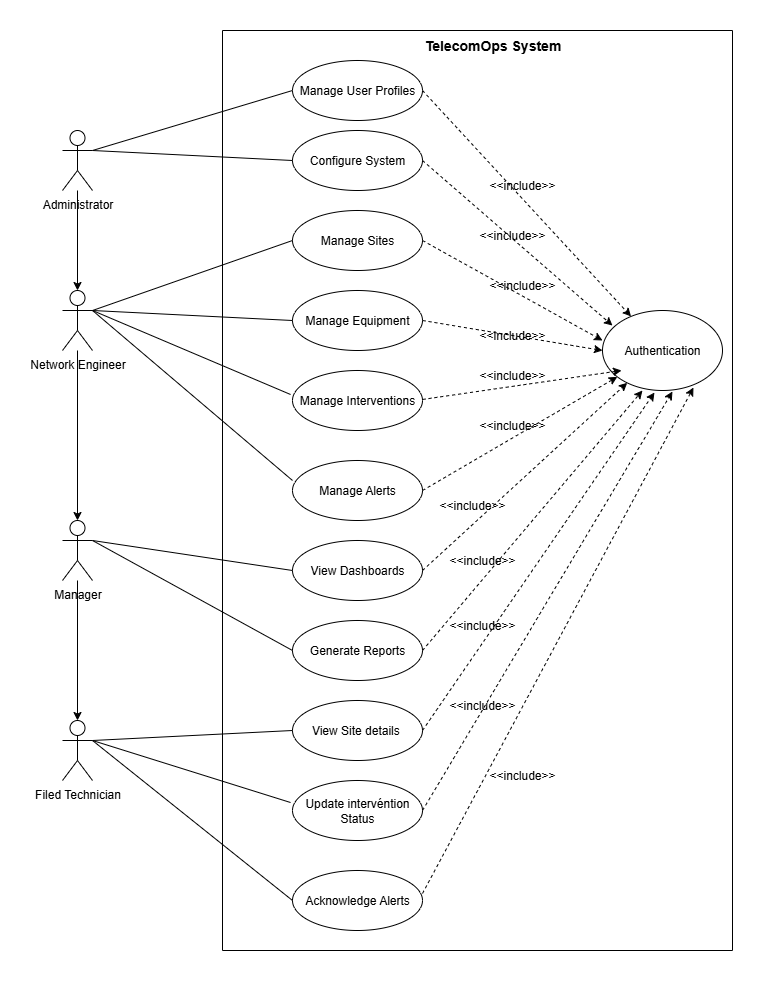
\includegraphics[width=0.95\linewidth]{img/chap_02/TelecomOps_UseCase_Diagram.png}
    \caption{Global Use Case Diagram}
    \label{fig:use_case_global}
\end{figure}
\vspace{1cm}

\section{System Architecture}
In this section, we describe the complete system architecture of the TelecomOps application, including the technological stack, component interactions, and deployment strategy.

\subsection{Architecture Overview}
The TelecomOps system follows a modern three-tier architecture built with Next.js for the frontend and Supabase for backend services. The architecture ensures clear separation of concerns, scalability, and maintainability. The main components include the presentation layer (Next.js), application layer (Supabase), and data layer (PostgreSQL).

\begin{figure}[hbt!]
    \centering
    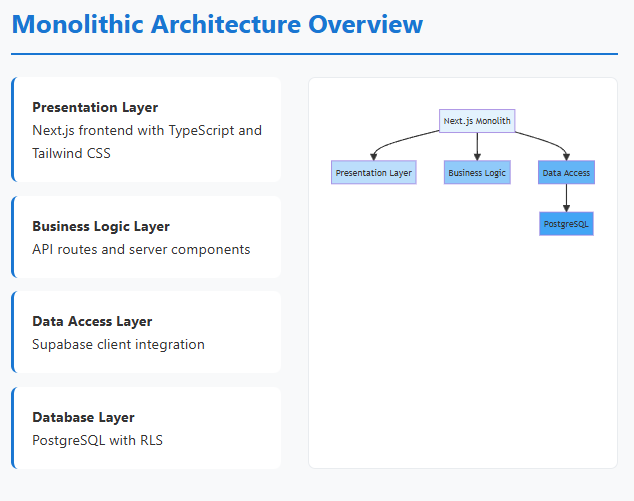
\includegraphics[width=0.9\linewidth]{img/chap_02/architecture_overview.png}
    \caption{Three-Tier Architecture Overview}
    \label{fig:architecture_overview}
\end{figure}

\subsection{Technology Stack}
The application utilizes a modern technology stack that ensures performance, scalability, and developer productivity:

\begin{itemize}
\item \textbf{Frontend:} Next.js 14 with TypeScript and Tailwind CSS
\item \textbf{Backend:} Supabase (PostgreSQL, Authentication, Real-time)
\item \textbf{Deployment:} Vercel (Frontend) and Supabase Cloud (Backend)
\item \textbf{Database:} PostgreSQL with Row Level Security
\end{itemize}

\begin{figure}[hbt!]
    \centering
    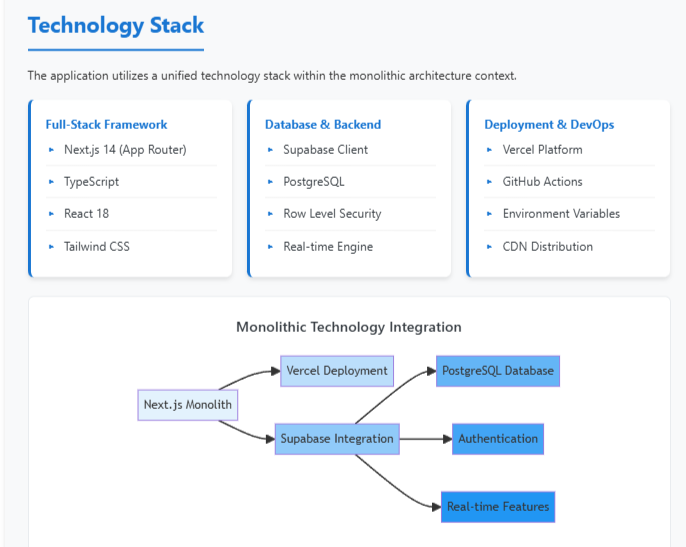
\includegraphics[width=0.85\linewidth]{img/chap_02/technology_stack.png}
    \caption{Technology Stack Components}
    \label{fig:technology_stack}
\end{figure}

\subsection{Database Architecture}
The database schema is designed to efficiently manage telecommunications site data, equipment, interventions, and alerts. The entity-relationship diagram below illustrates the comprehensive data model.

\begin{figure}[hbt!]
    \centering
    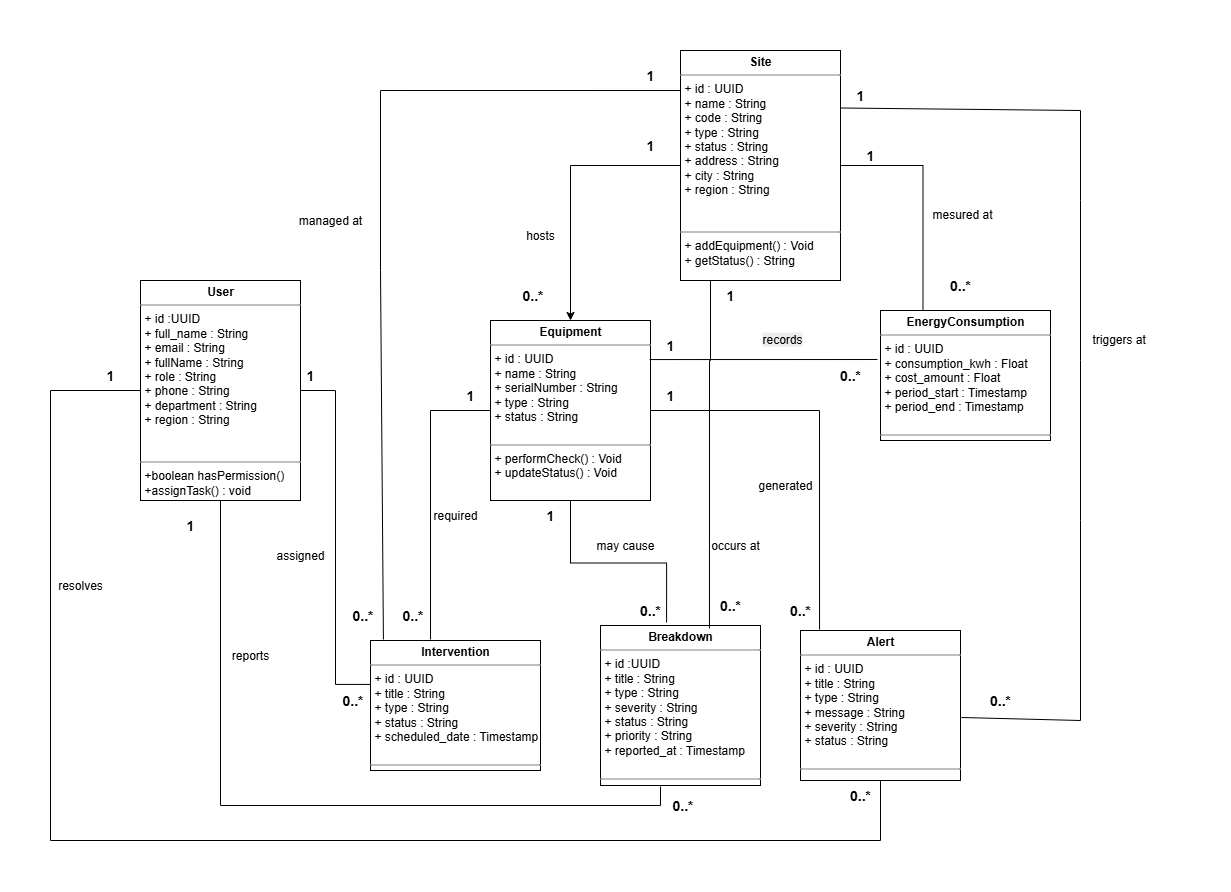
\includegraphics[width=0.95\linewidth]{img/chap_02/database_er_diagram.png}
    \caption{Database Entity-Relationship Diagram}
    \label{fig:database_er_diagram}
\end{figure}

\subsection{Data Flow Architecture}
The system follows a structured data flow pattern where user interactions are processed through multiple layers, ensuring security and data consistency at each step.

\begin{figure}[hbt!]
    \centering
    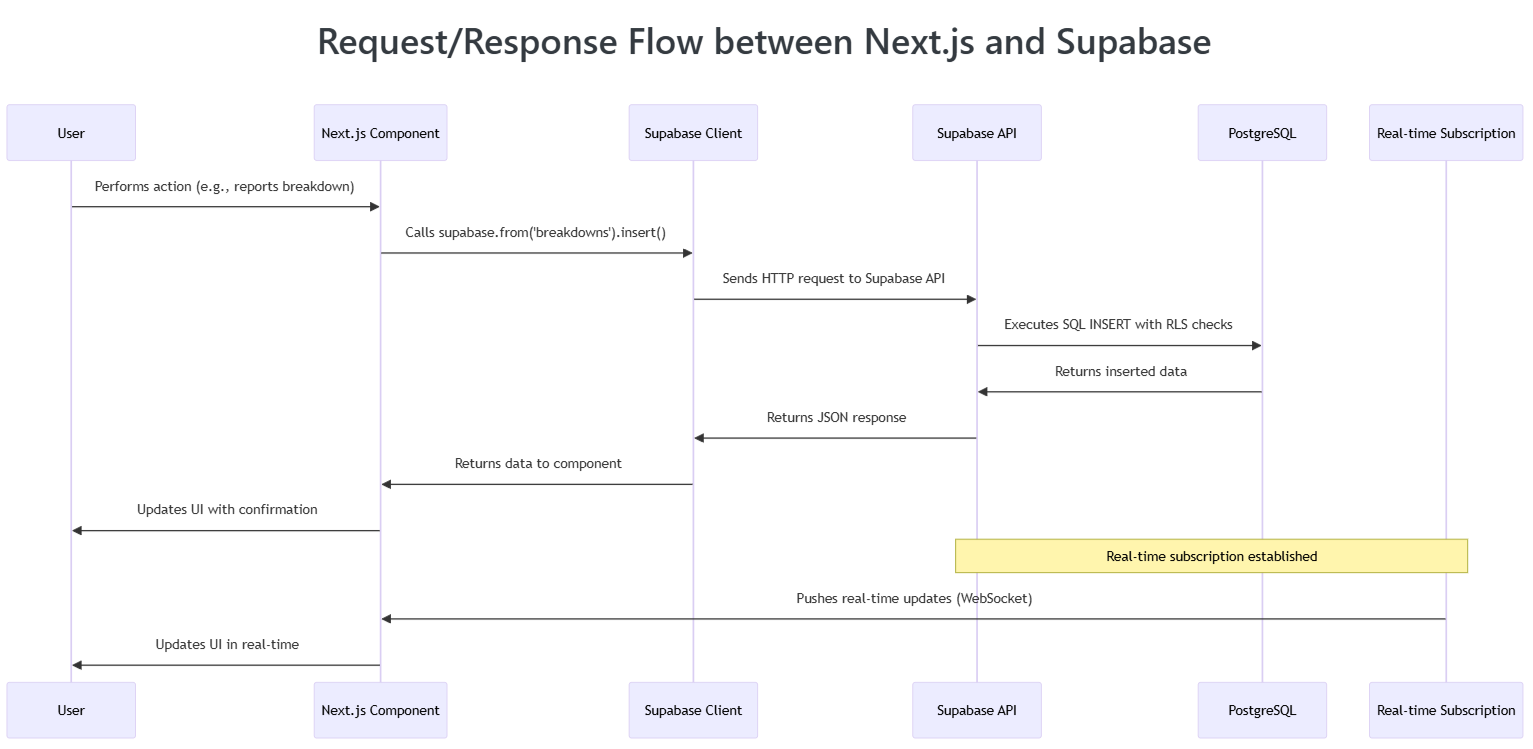
\includegraphics[width=0.9\linewidth]{img/chap_02/data_flow_architecture.png}
    \caption{Data Flow Architecture}
    \label{fig:data_flow_architecture}
\end{figure}

\subsection{Security Architecture}
Security is implemented at multiple layers, including transport security, application-level authentication, and database row-level security policies.

\begin{figure}[hbt!]
    \centering
    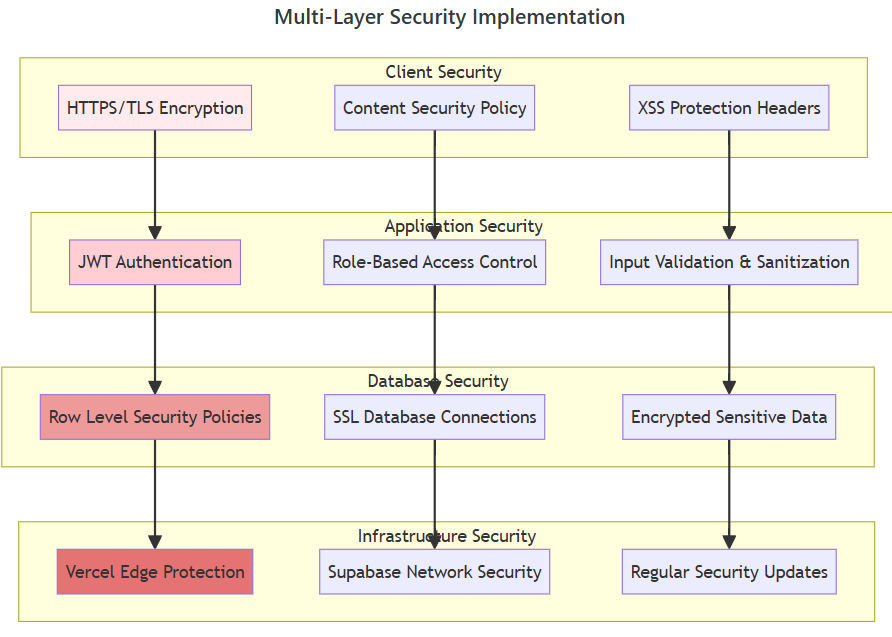
\includegraphics[width=1\linewidth]{img/chap_02/security_architecture.png}
    \caption{Multi-Layer Security Architecture}
    \label{fig:security_architecture}
\end{figure}

\subsection{Deployment Architecture}
The application is deployed using modern cloud platforms that provide scalability, reliability, and global availability.

\begin{figure}[hbt!]
    \centering
    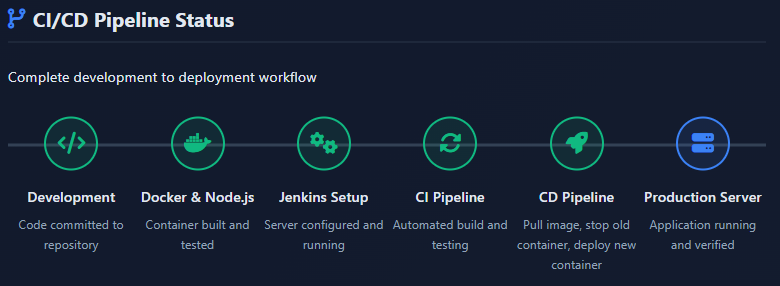
\includegraphics[width=0.85\linewidth]{img/chap_02/deployment_architecture.png}
    \caption{Cloud Deployment Architecture}
    \label{fig:deployment_architecture}
\end{figure}

\subsection{Component Interactions}
The system components interact through well-defined APIs and real-time subscriptions, ensuring efficient communication between the frontend and backend services.

\subsubsection{Next.js Frontend}
The Next.js application handles both server-side rendering and client-side interactions, providing a seamless user experience while maintaining optimal performance.

\subsubsection{Supabase Backend Services}
Supabase provides multiple backend services including:
\begin{itemize}
\item Authentication and authorization management
\item Auto-generated REST APIs from database schema
\item Real-time subscriptions for live data updates
\item File storage and management
\end{itemize}

\subsubsection{PostgreSQL Database}
The PostgreSQL database implements Row Level Security (RLS) policies to ensure data access is strictly controlled based on user roles and permissions.

\subsection{Architecture Benefits}
The chosen architecture provides several significant advantages:

\begin{itemize}
\item \textbf{Scalability:} Cloud-native design allows horizontal scaling
\item \textbf{Maintainability:} Clear separation of concerns simplifies updates
\item \textbf{Security:} Multi-layer security implementation protects sensitive data
\item \textbf{Performance:} Server-side rendering and CDN distribution ensure fast loading
\item \textbf{Real-time Capabilities:} WebSocket connections enable live updates
\end{itemize}

\section{Application Security}
Security is an essential aspect in any web application, especially when it comes to protecting sensitive data and ensuring that only authorized people can access resources. In this project, we have adopted a modern approach to manage user authentication and authorization by integrating Supabase, an open-source Backend-as-a-Service platform.

\subsection{Definition of Supabase}
Supabase is an open-source Backend-as-a-Service platform that provides database, authentication, real-time subscriptions, and API services. It allows centralized management of user identities and access for modern applications.

\subsection{Supabase Security Features}
Supabase ensures unified identity and access management, based on several key features that structure its operation:

\vspace{0.5cm}

\begin{itemize}
\item \textbf{User and Role Management:} \\
Users are created and managed through Supabase authentication system and each user can be assigned to one or more roles. Roles determine user permissions in the application based on their job function (Administrator, Network Engineer, Field Technician, Manager).

\vspace{0.5cm}

\item \textbf{Authentication Process:} \\
When the user attempts to log in, they interact directly with Supabase secure authentication service.
After successful login verification, Supabase generates an access token (JWT) containing user information (name, email, role, permissions) and returns it to the application.

\vspace{0.5cm}

\item \textbf{Authorization Control:} \\
The system verifies the access token received in each request to ensure that the user has the necessary permissions to access the requested resource or perform the requested action.
\end{itemize}

\subsection{Interaction with Application Components}
In a modern architecture, interaction between different systems relies on efficient authentication and authorization management. Here is a detailed overview of the flow and integrations necessary to ensure this communication.

\vspace{0.5cm}

\begin{itemize}
\item \textbf{Frontend Application:} \\
The frontend, developed with Next.js and TypeScript, uses Supabase JavaScript client library to manage user authentication. When a user attempts to access the TelecomOps application, Supabase checks if they are already logged in. If not, the user is redirected to the secure login interface to enter their credentials. Once authenticated, Supabase returns an access token that the frontend stores securely. This token is then included in requests sent to API endpoints, enabling access to secured telecom operations. This flow ensures centralized authentication and secure communication between different parts of the application.

\vspace{0.5cm}

\item \textbf{Backend API System:} \\
The backend, built with Next.js API routes, is configured to validate access tokens generated by Supabase using secure server-side libraries. Each request sent to API endpoints must include a valid token in the HTTP header in the form Authorization: Bearer <token>. When receiving a request, the backend decodes this token to verify the user identity and role-based permissions. Access to different API endpoints (sites management, equipment tracking, interventions, alerts) is then controlled using middleware and Row Level Security policies, ensuring precise authorization control for telecom operations.

\vspace{0.5cm}

\item \textbf{Database Security (PostgreSQL):} \\
Business data, such as site information, equipment details, maintenance interventions, and network alerts, are stored in a PostgreSQL database managed by Supabase. Supabase ensures security through Row Level Security (RLS) policies that guarantee only authorized requests reach the database based on user roles and permissions. Once these requests are validated, they are processed normally on the PostgreSQL database with additional security layers protecting sensitive telecom infrastructure data.
\end{itemize}

\subsection{Global Security Flow}
The global security flow described below illustrates the different stages of secure interaction between systems:

\begin{enumerate}
\item The user attempts to access the TelecomOps application via the web interface.
\item Supabase authenticates the user credentials and generates a secure access token.
\item The frontend sends requests to API endpoints with the access token included.
\item The backend verifies the token with Supabase and authorizes or denies the request based on user roles and permissions.
\item If authorized, the backend executes the telecom operation on PostgreSQL and returns the secure response to the frontend.
\end{enumerate}

\begin{figure}[H]
    \centering
    \includegraphics[width=1\linewidth]{img/architecture/supabase_security_flow.png}
    \caption{Global Security Flow of TelecomOps Authentication}
    \label{fig:security_flow}
\end{figure}

\subsection{Security Benefits}
The Supabase security implementation provides several advantages for the TelecomOps system:

\vspace{0.5cm}

\begin{itemize}
\item \textbf{Centralized Security Management:} \\
All authentication and authorization logic is handled by Supabase, reducing security complexity and potential vulnerabilities.

\vspace{0.5cm}

\item \textbf{Role-Based Access Control:} \\
Different user types (Administrator, Network Engineer, Field Technician, Manager) have appropriate access levels to telecom operations and sensitive network data.

\vspace{0.5cm}

\item \textbf{Data Protection:} \\
Row Level Security policies ensure that users can only access telecom site data and equipment information relevant to their role and assigned responsibilities.

\vspace{0.5cm}

\item \textbf{Secure Communication:} \\
All data transmission between components uses encrypted HTTPS connections with JWT token validation for additional security layers.
\end{itemize}
        \clearpage
        
        \newpage

\chapter{Sprint 1: Site Management and Authentication}

\cfoot{\thepage}

\parindent=0.5in
\onehalfspacing

\usepackage{multirow}

\section{Introduction}

Sprint 1, titled "Site Management and Authentication," establishes the foundational elements essential for all subsequent development phases. This sprint focuses on implementing secure user access control with Supabase authentication and basic site information management capabilities required for telecommunications infrastructure operations.

The sprint addresses four high-priority user stories from Chapter 2's product backlog: US-001 (User Authentication), US-002 (User Profile Management), US-003A-C (Site Management CRUD operations), and US-004 (Site Information Access). These stories form the foundation upon which subsequent sprints build equipment monitoring, intervention planning, and analytics capabilities.

Sprint 1 objectives align with the architectural design presented in Chapter 2, implementing the authentication layer through Supabase Auth, establishing the initial database schema with profiles and sites tables, and creating the presentation layer foundation with Next.js and TypeScript. The implementation demonstrates the layered architecture's effectiveness while establishing role-based access control enforced at multiple levels.

\section{Sprint Backlog}

During sprint planning, we defined the tasks required for Sprint 1 implementation. Table 3.1 presents the sprint backlog with user stories, tasks, complexity assessments, and effort estimates in story points.

\begin{table}[H]
\centering
\small
\begin{tabular}{|p{2.5cm}|p{4cm}|p{3.2cm}|p{2.2cm}|p{1.5cm}|}
\hline
\textbf{Functionality} & \textbf{User Story} & \textbf{Tasks} & \textbf{Complexity} & \textbf{Estimate} \\
\hline

\multirow{3}{2.5cm}{Authentication System} & 
\multirow{3}{4cm}{As admin, engineer, technician, and manager, I can authenticate to access the system}
& Supabase Auth integration & Hard & 8 \\
\cline{3-5}
& & Create login interface & Medium & 3 \\
\cline{3-5}
& & Integration and testing & Hard & 5 \\
\hline

\multirow{3}{2.5cm}{User Profile Management} & 
\multirow{3}{4cm}{As any user, I want to manage my profile and change my password}
& Implement profile management & Medium & 3 \\
\cline{3-5}
& & Create profile interface & Easy & 2 \\
\cline{3-5}
& & Integration and testing & Medium & 3 \\
\hline

\multirow{3}{2.5cm}{Create Site (US-003A)} & 
\multirow{3}{4cm}{As admin, engineer, or manager, I can create new telecommunications sites}
& Implement site creation logic & Medium & 4 \\
\cline{3-5}
& & Create site creation modal & Medium & 3 \\
\cline{3-5}
& & Validation and testing & Medium & 3 \\
\hline

\multirow{3}{2.5cm}{Edit Site (US-003B)} & 
\multirow{3}{4cm}{As admin or engineer, I can edit existing site information. As manager, I can edit site status}
& Implement site edit logic & Medium & 3 \\
\cline{3-5}
& & Create site edit modal & Easy & 2 \\
\cline{3-5}
& & Permission testing & Medium & 3 \\
\hline

\multirow{3}{2.5cm}{Delete Site (US-003C)} & 
\multirow{3}{4cm}{As admin, I can delete decommissioned sites from the system}
& Implement site deletion & Easy & 2 \\
\cline{3-5}
& & Create confirmation modal & Easy & 1 \\
\cline{3-5}
& & Referential integrity testing & Medium & 3 \\
\hline

\multirow{3}{2.5cm}{View Sites (US-004)} & 
\multirow{3}{4cm}{As all users, I can view telecommunications site information}
& Implement site list view & Medium & 3 \\
\cline{3-5}
& & Create site detail view & Medium & 3 \\
\cline{3-5}
& & Real-time updates & Hard & 4 \\
\hline

\multirow{3}{2.5cm}{Role-Based Access Control} & 
\multirow{3}{4cm}{As the system, I enforce different access levels based on user roles}
& Implement RLS policies & Hard & 6 \\
\cline{3-5}
& & Configure role permissions & Medium & 3 \\
\cline{3-5}
& & Test all role combinations & Hard & 4 \\
\hline

\end{tabular}
\caption{Sprint 1 Backlog with Task Breakdown}
\label{tab:sprint1_backlog}
\end{table}

The backlog totals 71 story points across seven user stories, aligning with the two-week sprint duration. The Site Management functionality has been split into three distinct user stories (US-003A, US-003B, US-003C) reflecting the different permission levels and operational contexts: site creation available to administrators, engineers, and managers; site editing with differentiated permissions; and site deletion restricted to administrators only. This granular approach enables precise permission management and facilitates sprint planning.

\section{Conceptual Design}

This section presents the conceptual design models guiding Sprint 1 implementation, ensuring alignment between requirements and technical implementation.

\subsection{Class Diagram}

Figure 3.1 presents the class diagram for Sprint 1, focusing on core entities: Supabase authentication, user profiles, and telecommunications sites.

\begin{figure}[H]
    \centering
    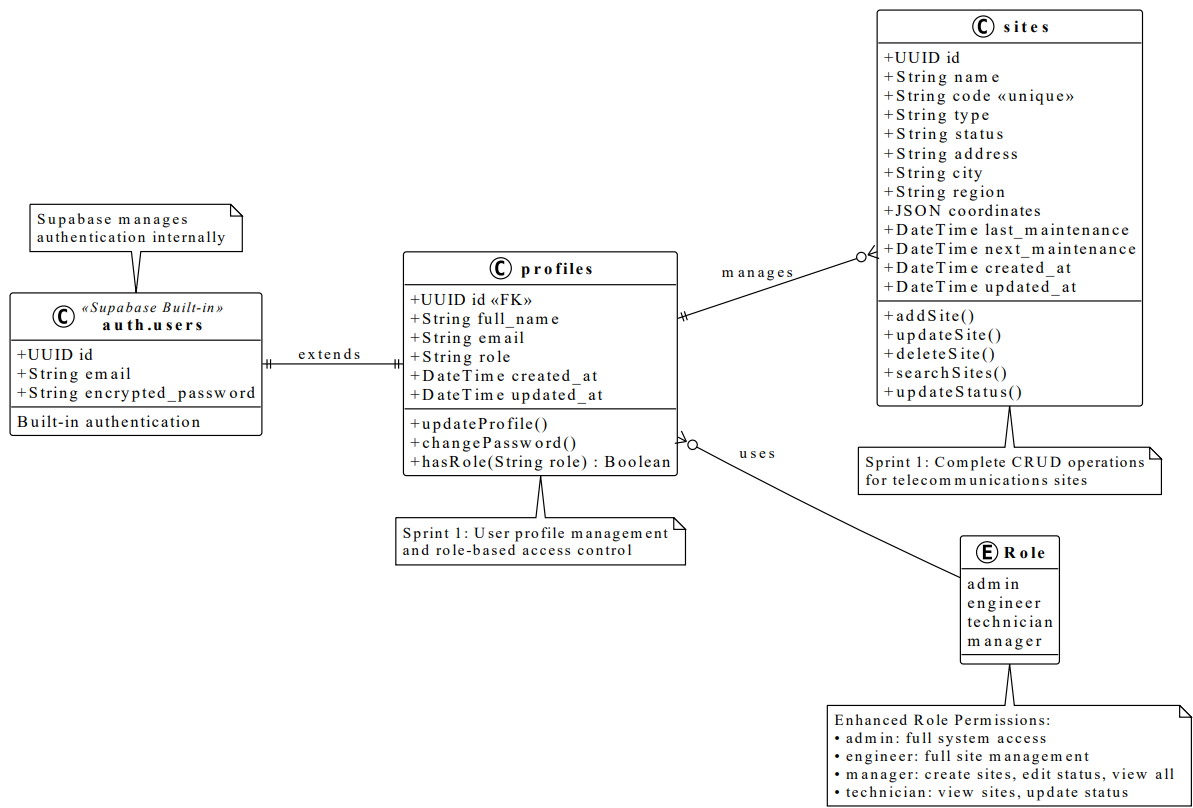
\includegraphics[width=0.95\linewidth]{img/chap_03/class_diagram_sprint1.png}
    \caption{Class Diagram - Authentication and Site Management}
    \label{fig:class_diagram_sprint1}
\end{figure}


The class diagram illustrates relationships between Supabase's built-in authentication system (\texttt{auth.users}), the custom \texttt{profiles} table extending user information with business-specific fields (role, region, full name), and the \texttt{sites} table for telecommunications site management. The \texttt{Role} enumeration defines four distinct user types (admin, engineer, technician, manager) corresponding to the stakeholder roles identified in Chapter 2. Each profile associates with exactly one authentication user, while sites maintain creation and modification audit trails through timestamps and user associations.

\subsection{Use Case Diagram}

Figure 3.2 presents the use case diagram showing actors and their interactions with Sprint 1 functionalities.

\begin{figure}[H]
    \centering
    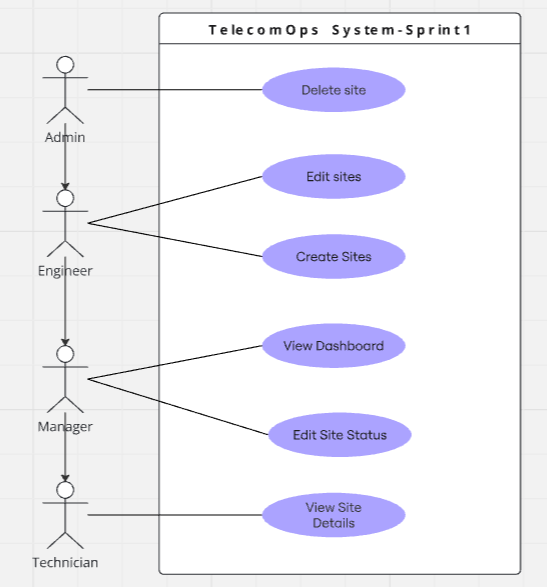
\includegraphics[width=0.85\linewidth]{img/chap_03/use_case_diagram_sprint1.png}
    \caption{Use Case Diagram - Sprint 1 Functionalities}
    \label{fig:use_case_diagram_sprint1}
\end{figure}

The use case diagram shows four primary actors with differentiated permission levels reflecting the stakeholder access matrix from Chapter 2, Table 2.1. Administrator has full system access including user management and site deletion. Network Engineer focuses on technical site management with create, edit, and view operations. Manager has operational oversight with site creation and status editing capabilities for deployment approvals and operational decisions. Field Technician has view access supporting field operations.

\textbf{Use Case Description: Create Site}

Since use cases for creating, editing, and deleting sites share similar processing patterns, we provide detailed information on the "Create Site" use case as representative of the site management functionality. Table 3.2 presents the detailed textual description.

\begin{table}[H]
\centering
\begin{tabular}{|p{3.5cm}|p{8cm}|}
\hline
\textbf{Use Case} & Create Site \\
\hline
\textbf{Primary Actors} & Administrator, Network Engineer, Manager \\
\hline
\textbf{Pre-condition} & User successfully authenticated with appropriate role (admin, engineer, or manager) \\
\hline
\textbf{Post-condition} & Site successfully created in database with unique identifier \\
\hline
\textbf{Main Scenario} & 
1. User accesses site management interface
2. User clicks "Add Site" button displaying creation modal
3. User fills form: name, code, address, coordinates, technology type
4. User submits form
5. System validates fields and checks site code uniqueness
6. System verifies user permissions via Row Level Security
7. System creates site in database
8. System updates site list in real-time
9. System displays success confirmation
\\
\hline
\textbf{Exception Scenarios} & 
E1: Missing required data → Display field-specific error messages
E2: Duplicate site code → Display uniqueness violation error
E3: Insufficient permissions → Display access denied error
E4: Server connection problem → Display connection error with retry option
\\
\hline
\end{tabular}
\caption{Detailed Use Case Description - Create Site}
\label{tab:create_site_usecase}
\end{table}

\section{Sequence Diagrams}

This section presents sequence diagrams detailing the main processes implemented in Sprint 1, illustrating interactions between system components.

\subsection{Authentication Process}

Figure 3.3 illustrates the complete user authentication workflow using Supabase authentication services.

\begin{figure}[H]
    \centering
    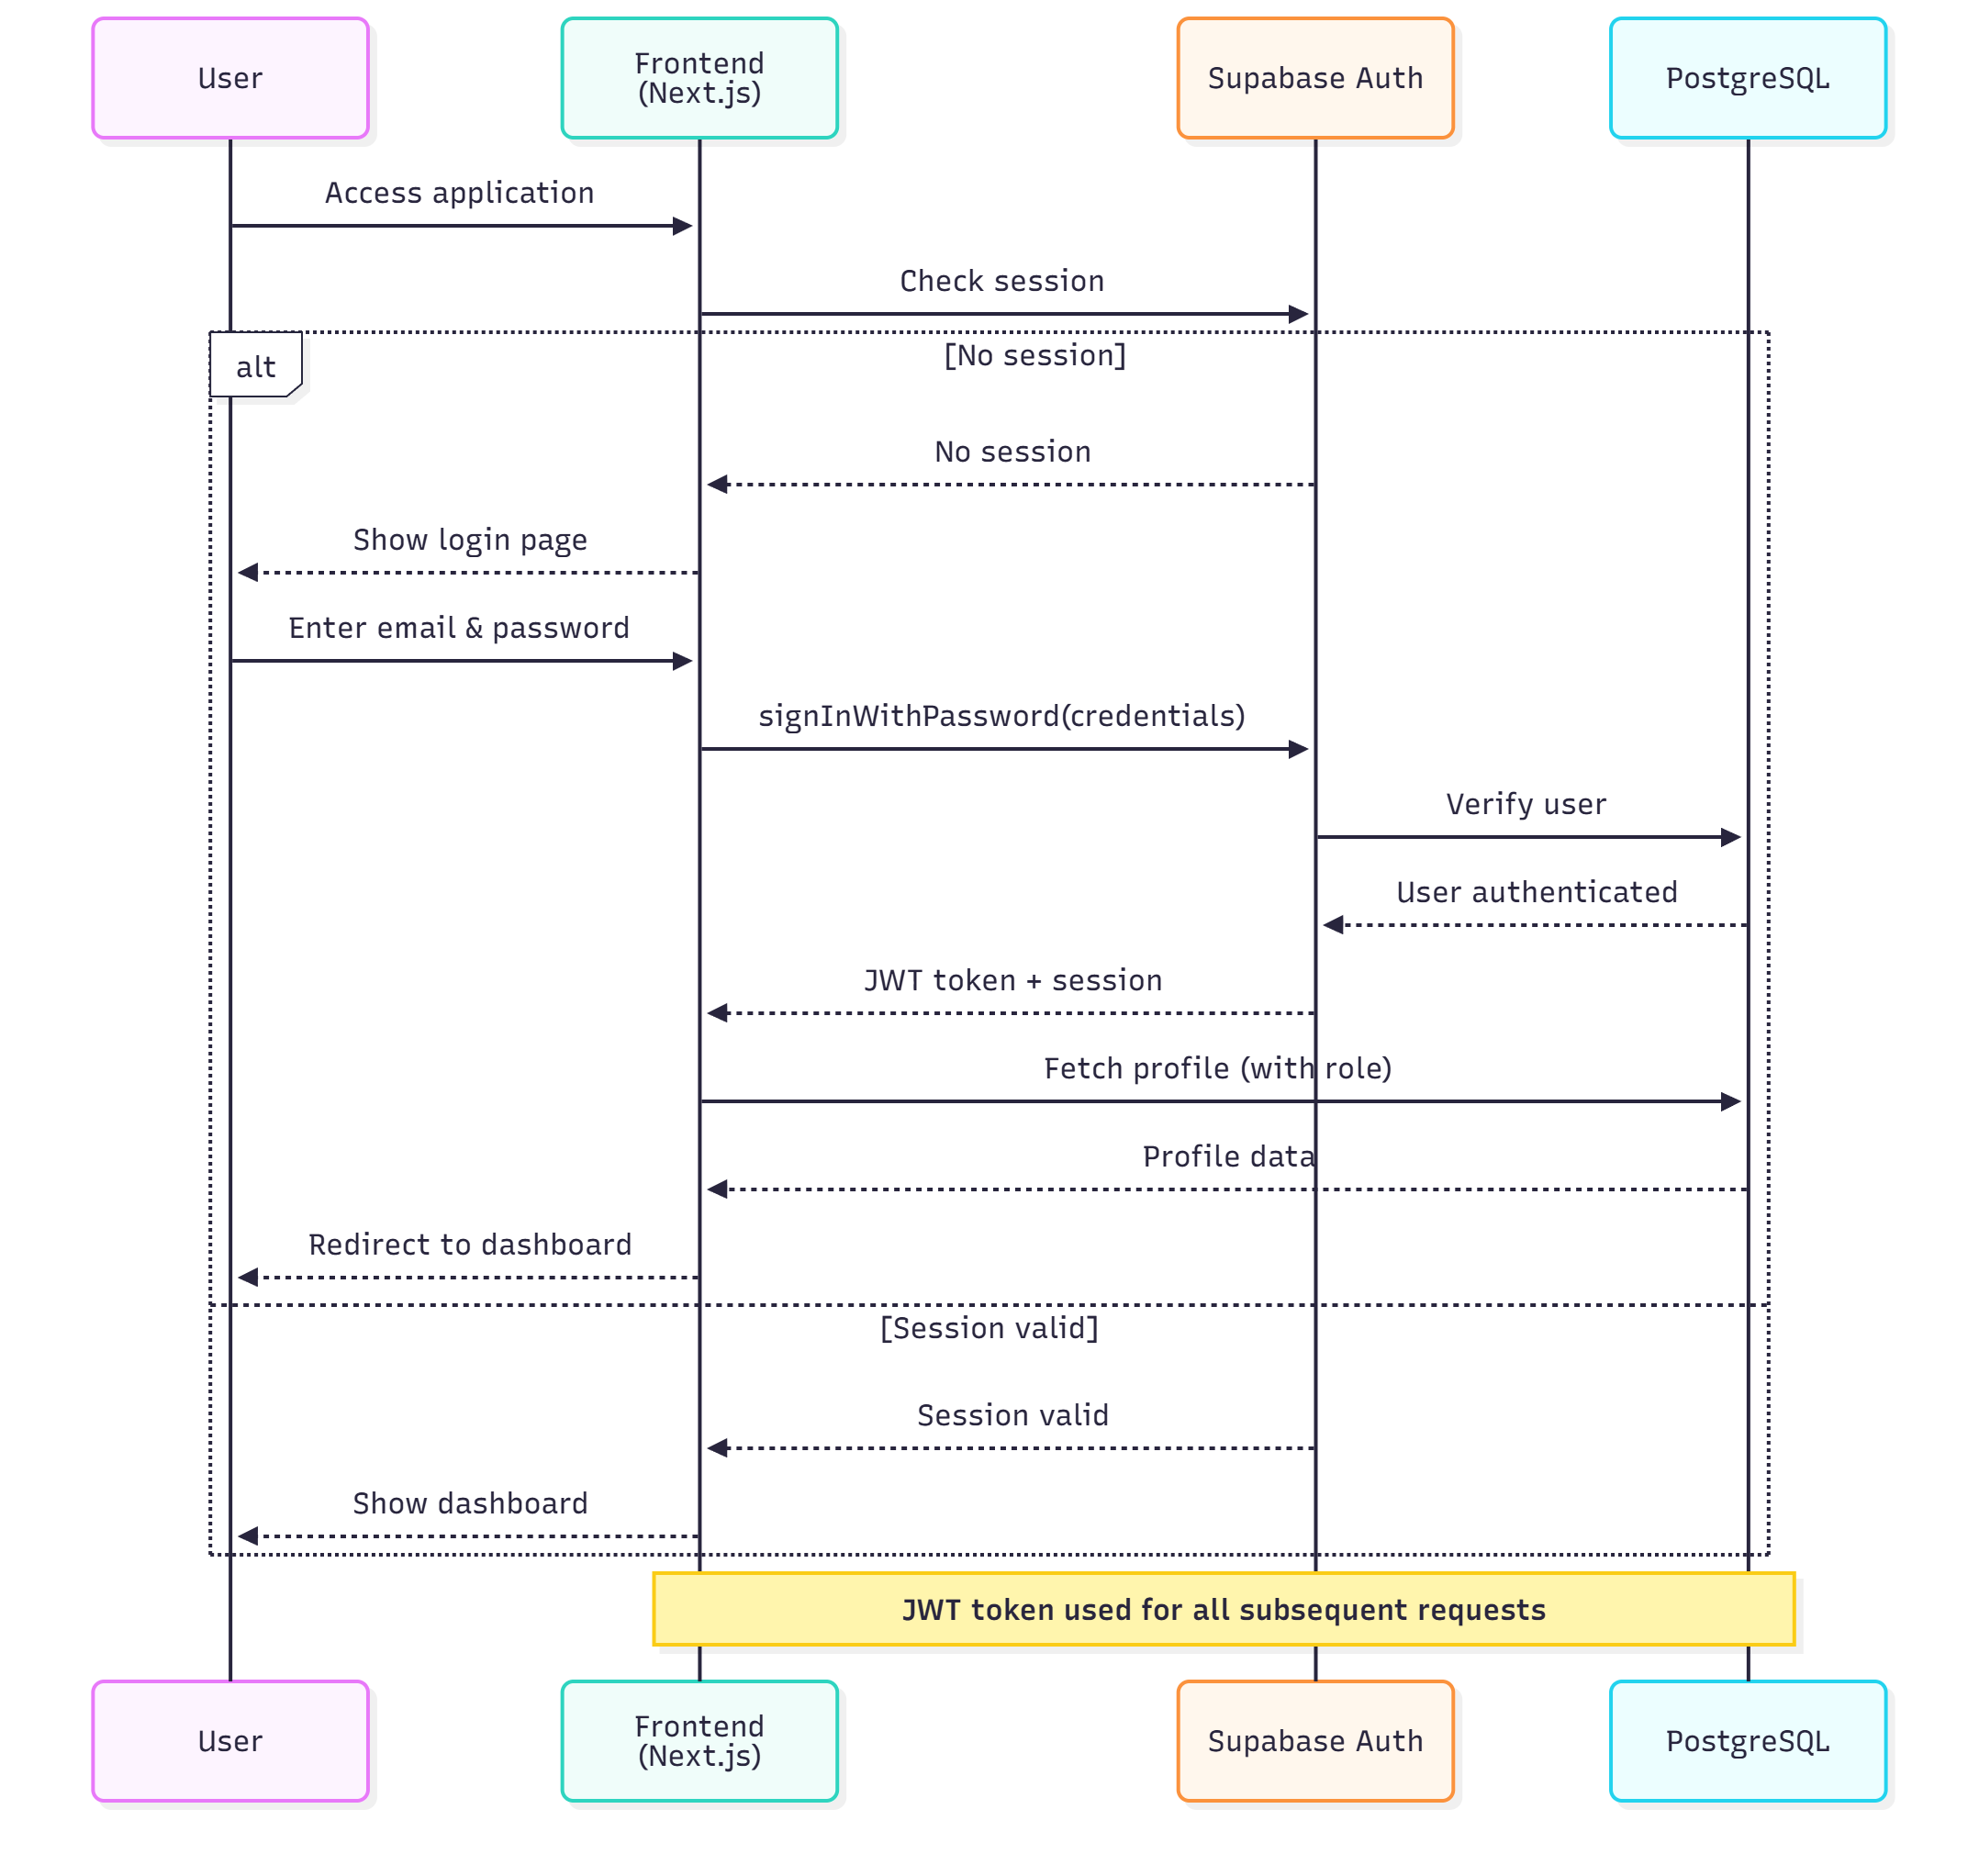
\includegraphics[width=0.95\linewidth]{img/chap_03/sequence_authentication.png}
    \caption{Sequence Diagram - Authentication Process}
    \label{fig:sequence_authentication}
\end{figure}

\textbf{Note on Sequence Diagram:} In proper UML sequence diagram notation, return messages should be represented with dashed lines (dotted lines) rather than solid lines, distinguishing them from request messages. The diagram should show request messages as solid arrows and return messages as dashed arrows to maintain standard UML conventions.

The authentication sequence (Figure 3.3) demonstrates the login process implementing Chapter 2's security architecture. When users access the application, the system checks for existing valid sessions. Without valid sessions, users enter credentials which undergo client-side validation before transmission to Supabase Auth via \texttt{signInWithPassword()}. Supabase verifies credentials against PostgreSQL, generates JWT tokens containing user identification upon success, and returns session information. The frontend fetches user profiles including roles using Row Level Security-protected queries, stores sessions locally, and redirects users to role-appropriate dashboards. Failed authentication displays error messages, while valid existing sessions grant direct dashboard access.

\subsection{Site Creation Process}

Figure 3.4 demonstrates the complete workflow for adding telecommunications sites to the system.

\begin{figure}[H]
    \centering
    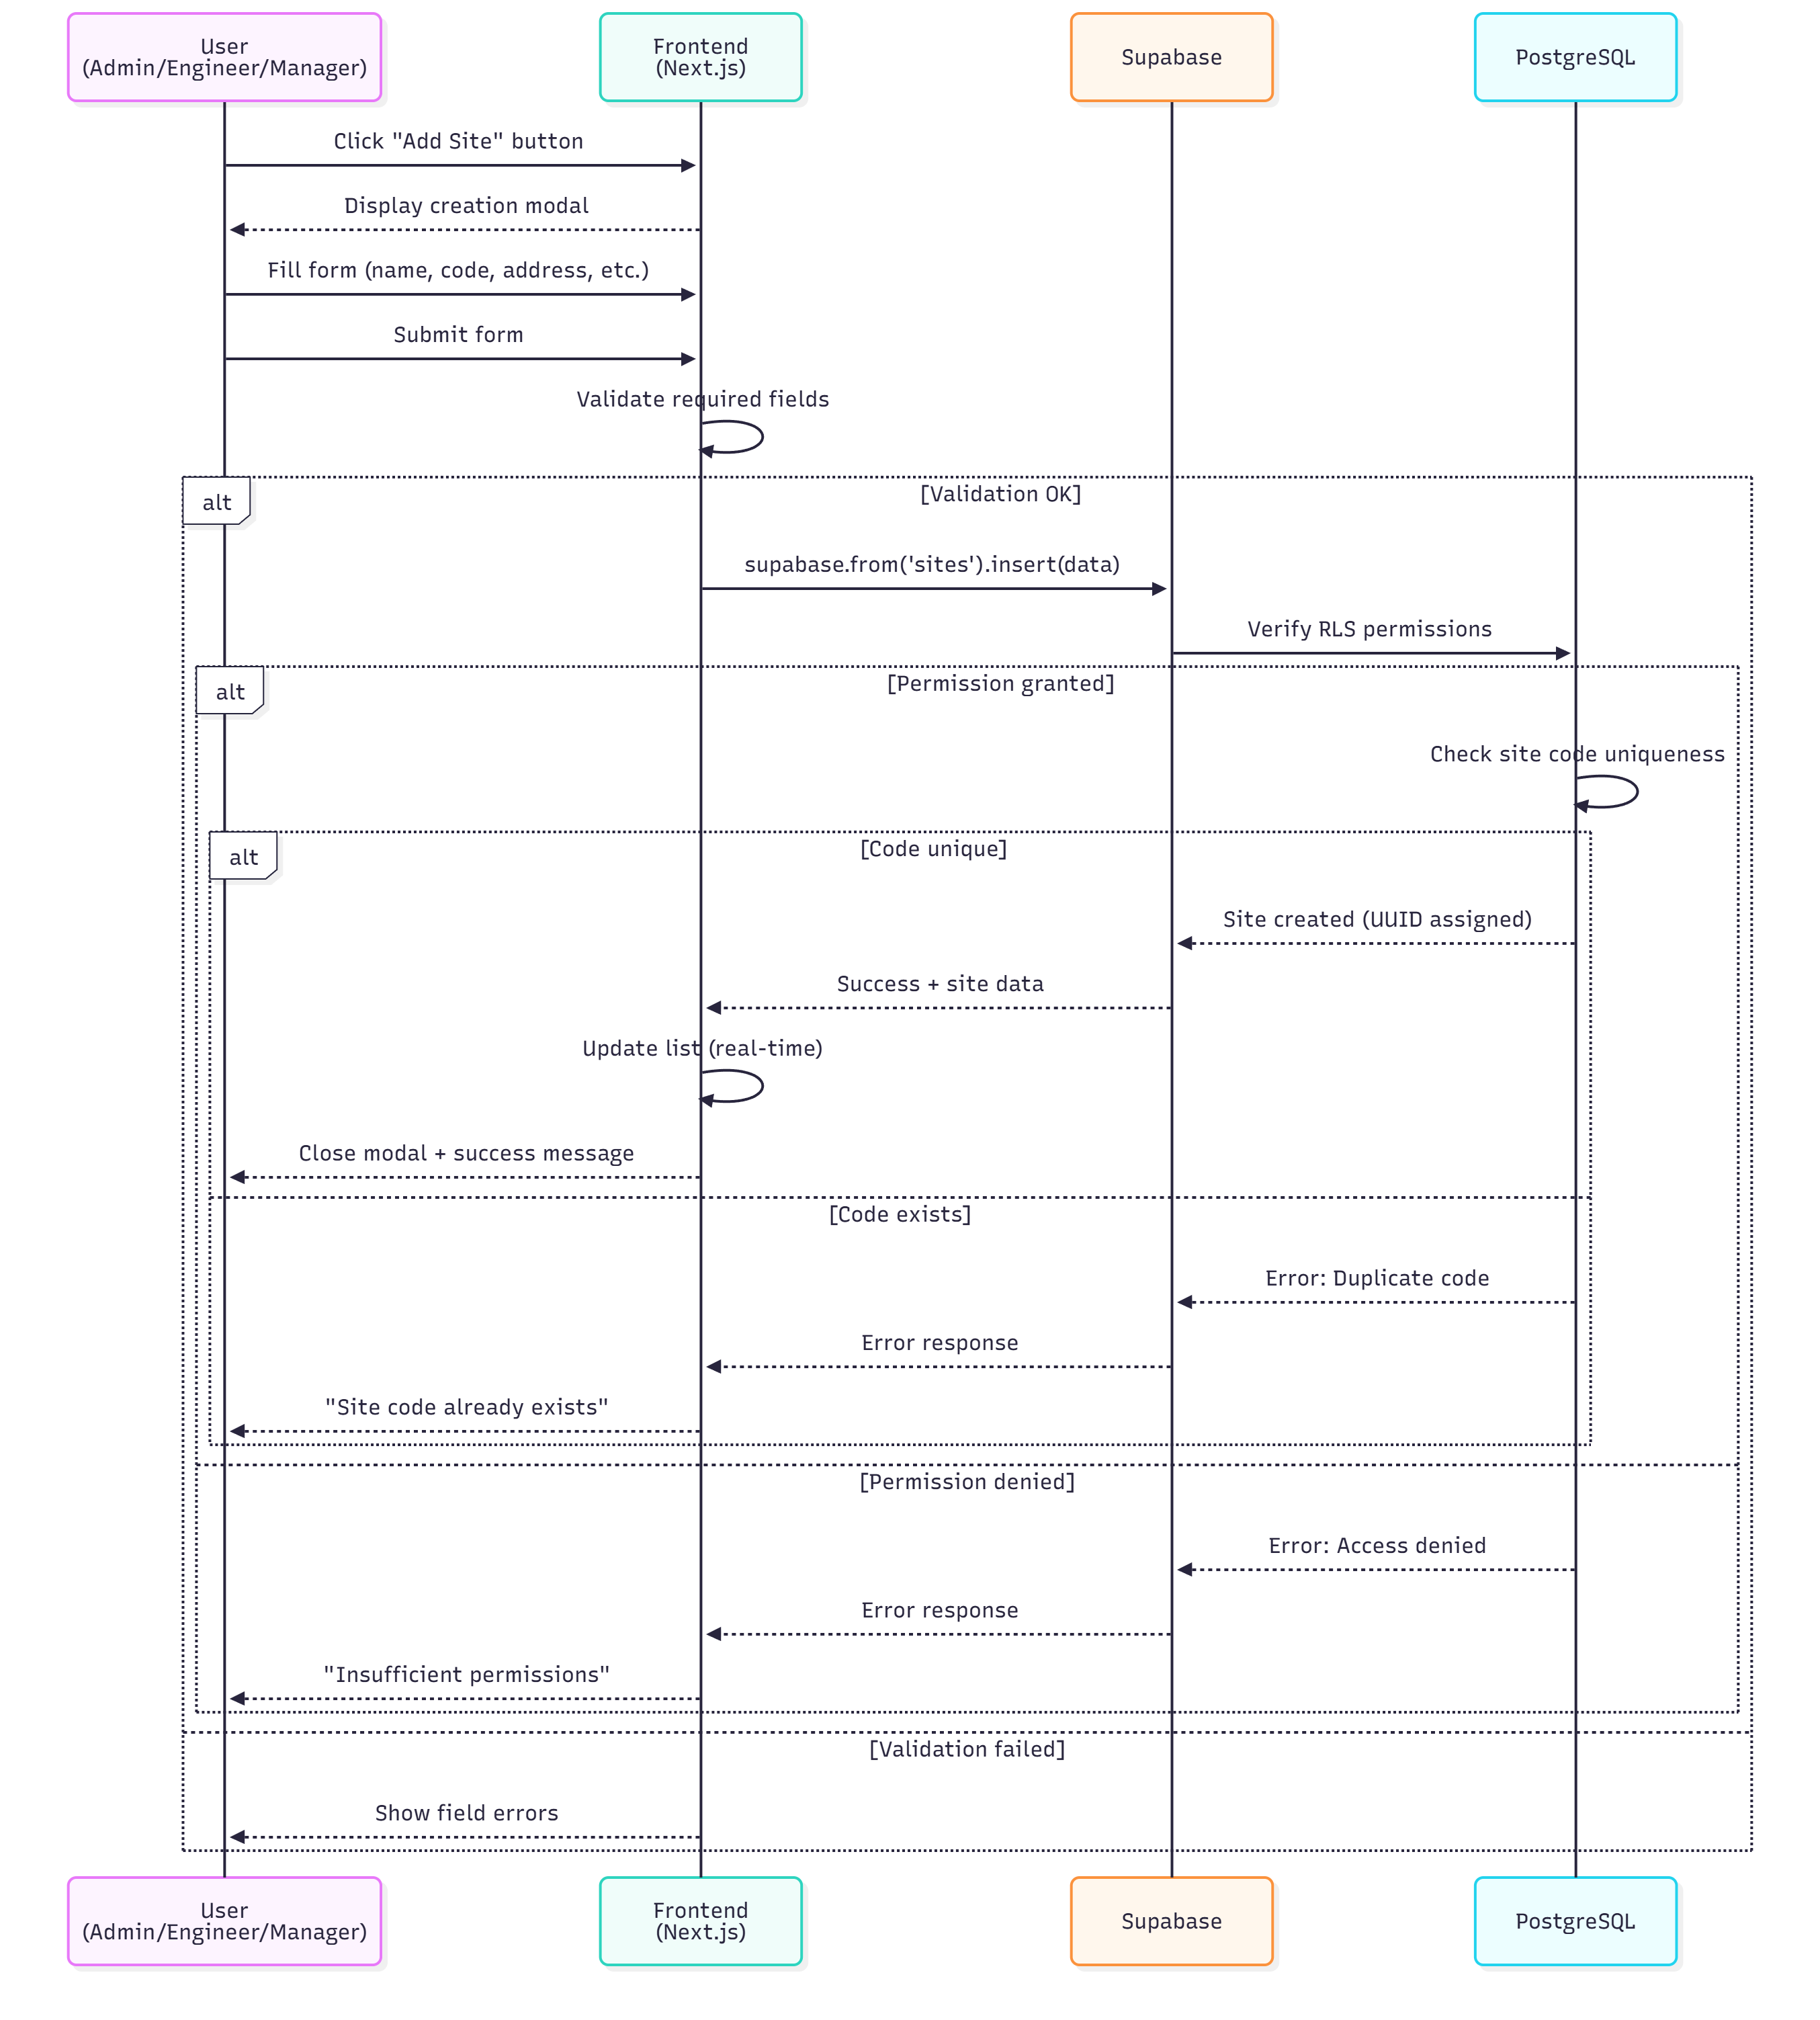
\includegraphics[width=0.95\linewidth]{img/chap_03/sequence_add_site.png}
    \caption{Sequence Diagram - Create Site Process}
    \label{fig:sequence_add_site}
\end{figure}

The site creation sequence (Figure 3.4) shows authorized users (Administrator, Engineer, Manager) accessing the site management interface and clicking "Add Site" to display the creation modal. After completing site details (name, unique code, address, technology type), form submission triggers comprehensive validation checking required fields and code format. Valid requests proceed to Supabase database via \texttt{supabase.from('sites').insert()}. The database performs two critical security checks: Row Level Security policy validation ensuring only authorized roles can create sites, and unique constraint checking preventing duplicate site codes. Successful validation results in site insertion with UUID assignment, real-time list updates via Supabase subscriptions, modal closure, and success confirmation. Constraint violations or validation failures display appropriate error messages guiding corrective action.

\section{Implementation}

This section presents screenshots illustrating the interfaces developed during Sprint 1 implementation, demonstrating the application's user experience design.

\subsection{Authentication Interface}

Figure 3.5 illustrates the authentication interface implementing Supabase's secure authentication system with email and password validation.

\begin{figure}[H]
    \centering
    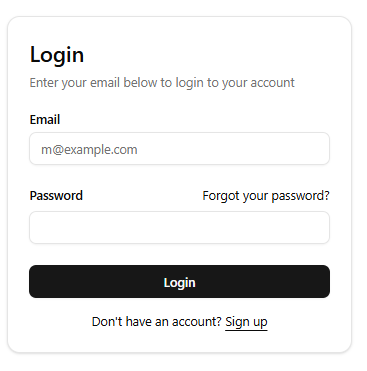
\includegraphics[width=0.7\linewidth]{img/chap_03/login_interface.png}
    \caption{Login Interface with Supabase Authentication}
    \label{fig:login_interface}
\end{figure}

\subsection{Dashboard Interfaces}

Figures 3.6 and 3.7 illustrate the role-based dashboard providing different views based on user roles, with the main dashboard showing key metrics and the sites management interface displaying the comprehensive site list with action buttons.

\begin{figure}[H]
    \centering
    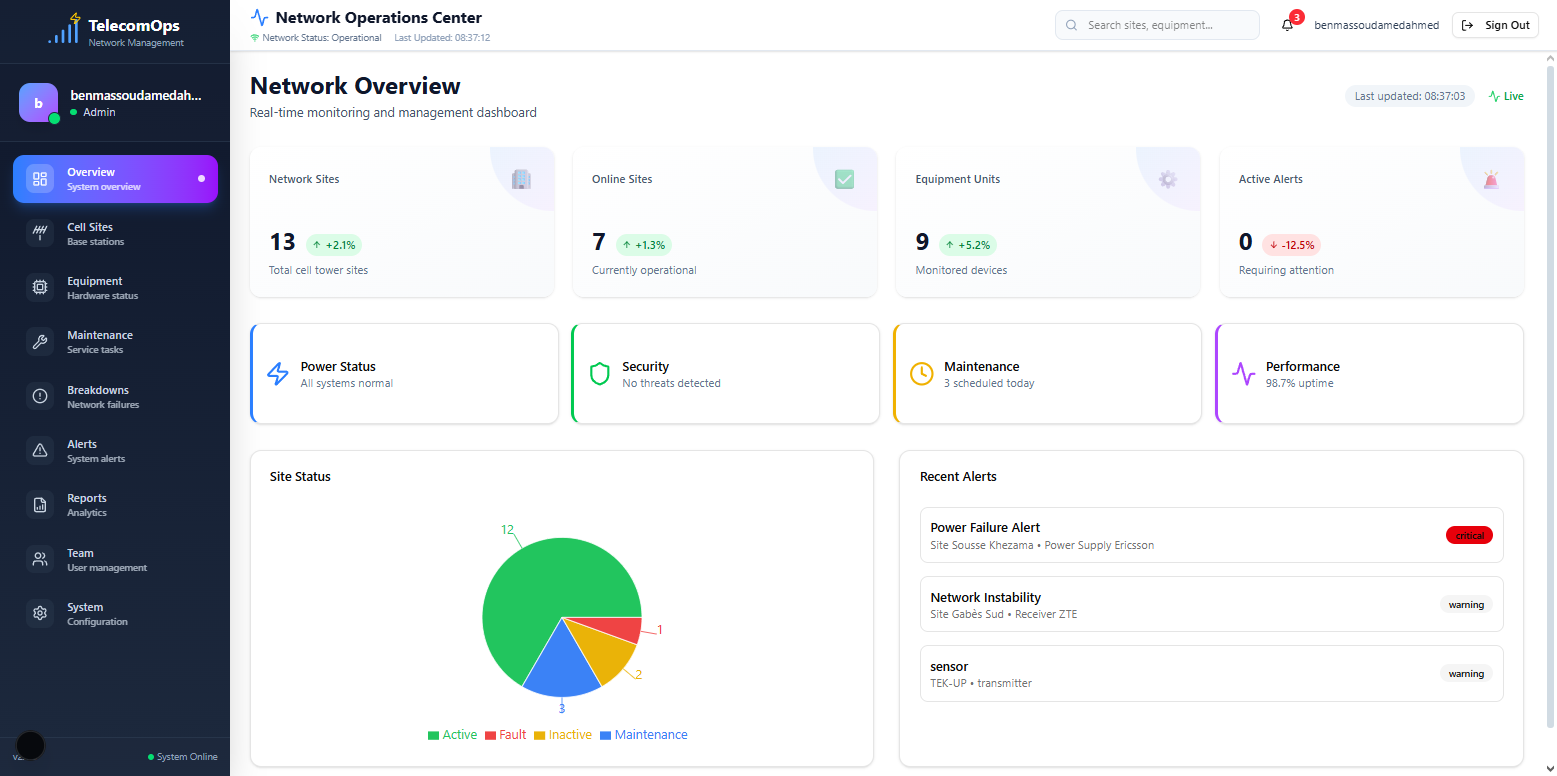
\includegraphics[width=0.9\linewidth]{img/chap_03/dashboard_main.png}
    \caption{Main Dashboard with Role-Based Metrics}
    \label{fig:dashboard_main}
\end{figure}

\begin{figure}[H]
    \centering
    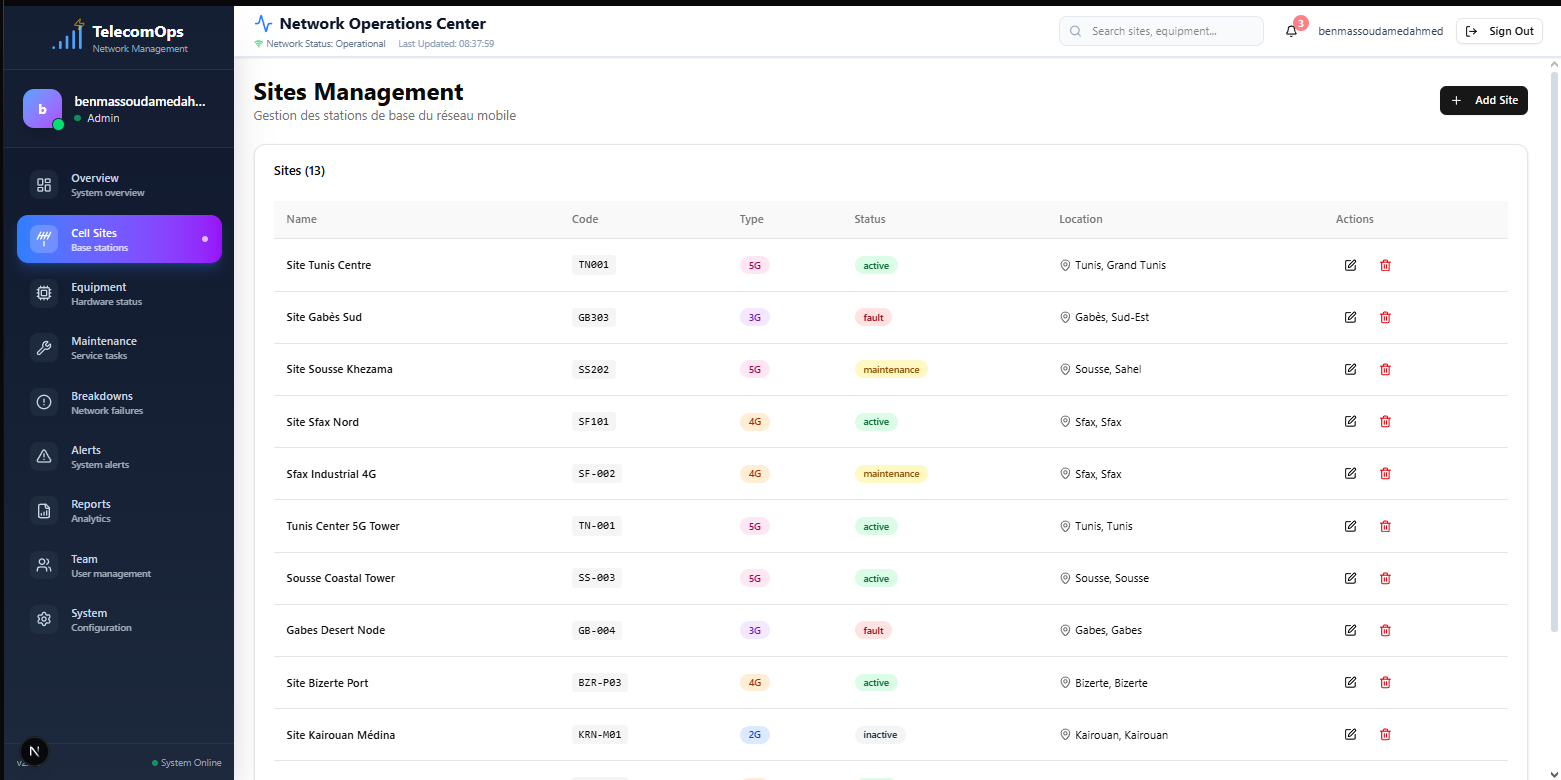
\includegraphics[width=0.9\linewidth]{img/chap_03/sites_list.png}
    \caption{Sites Management Interface with Action Controls}
    \label{fig:sites_list}
\end{figure}

\subsection{Site Management Modals}

Figures 3.8, 3.9, and 3.10 illustrate the site management modals implementing the CRUD operations with appropriate permission checks enforced through Row Level Security.

\begin{figure}[H]
    \centering
    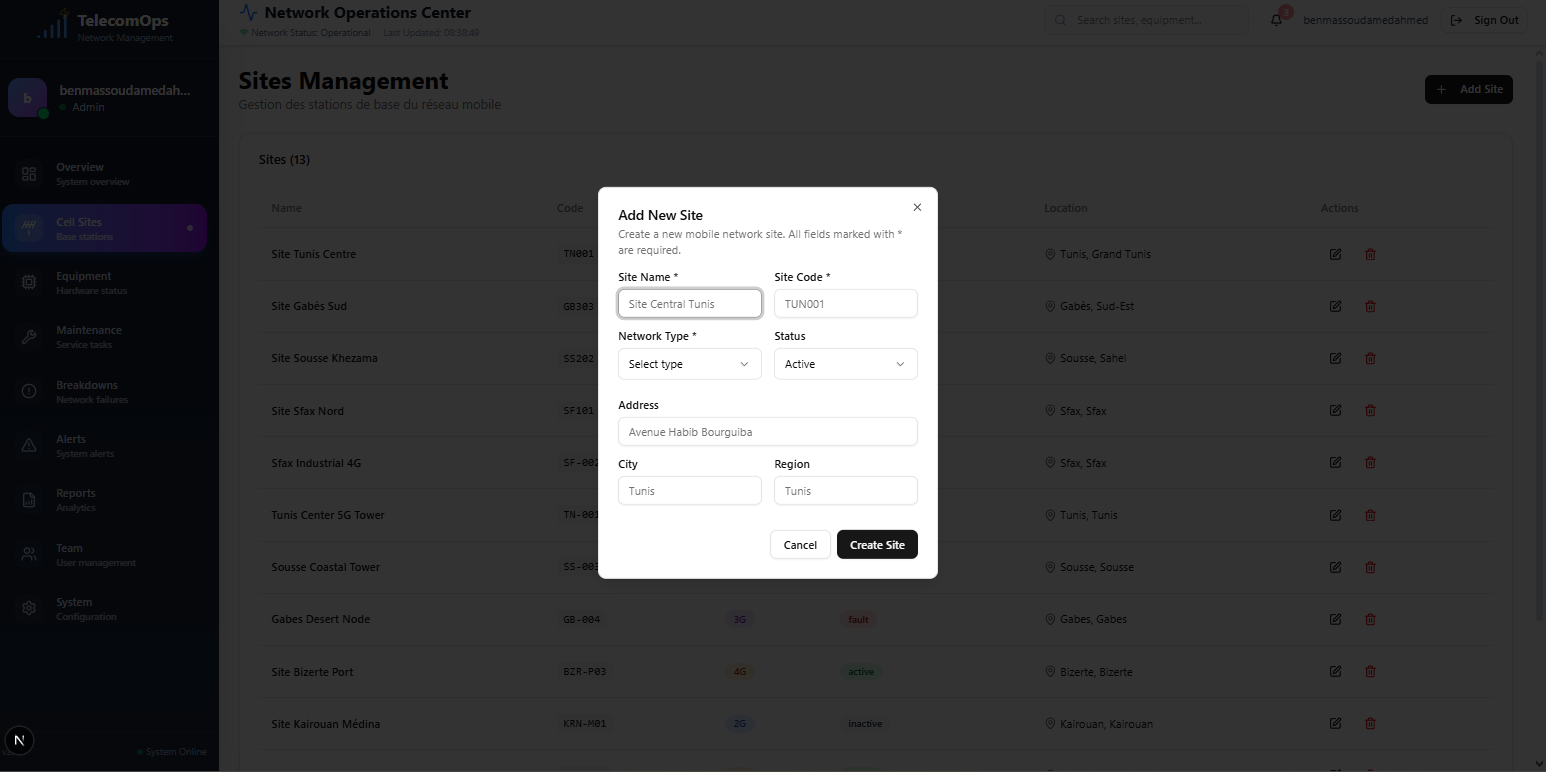
\includegraphics[width=0.85\linewidth]{img/chap_03/create_site_modal.png}
    \caption{Create Site Modal with Form Validation}
    \label{fig:add_site_modal}
\end{figure}

\begin{figure}[H]
    \centering
    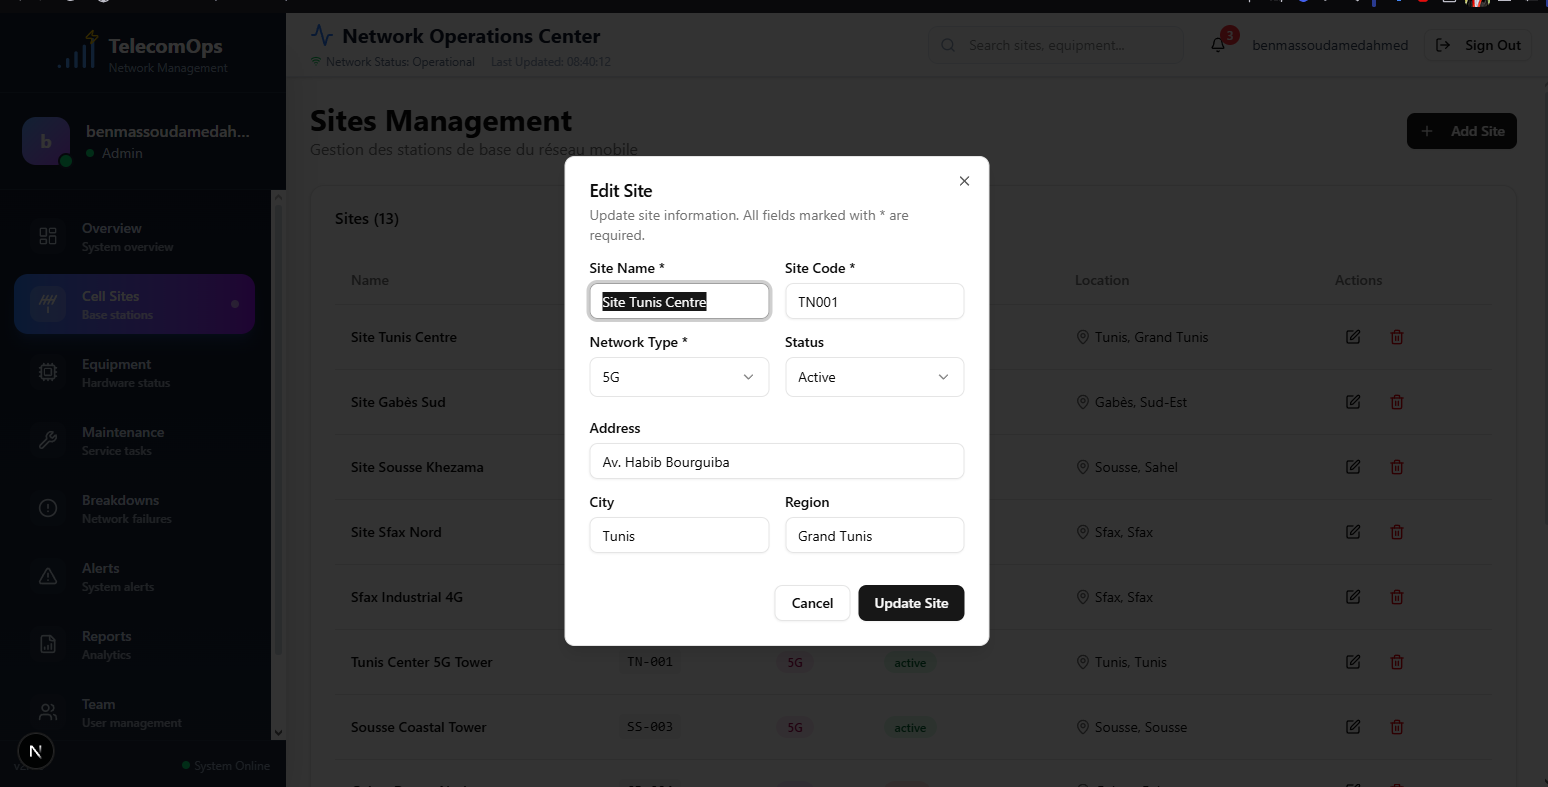
\includegraphics[width=0.85\linewidth]{img/chap_03/edit_site_modal.png}
    \caption{Edit Site Modal with Pre-populated Data}
    \label{fig:edit_site_modal}
\end{figure}

\begin{figure}[H]
    \centering
    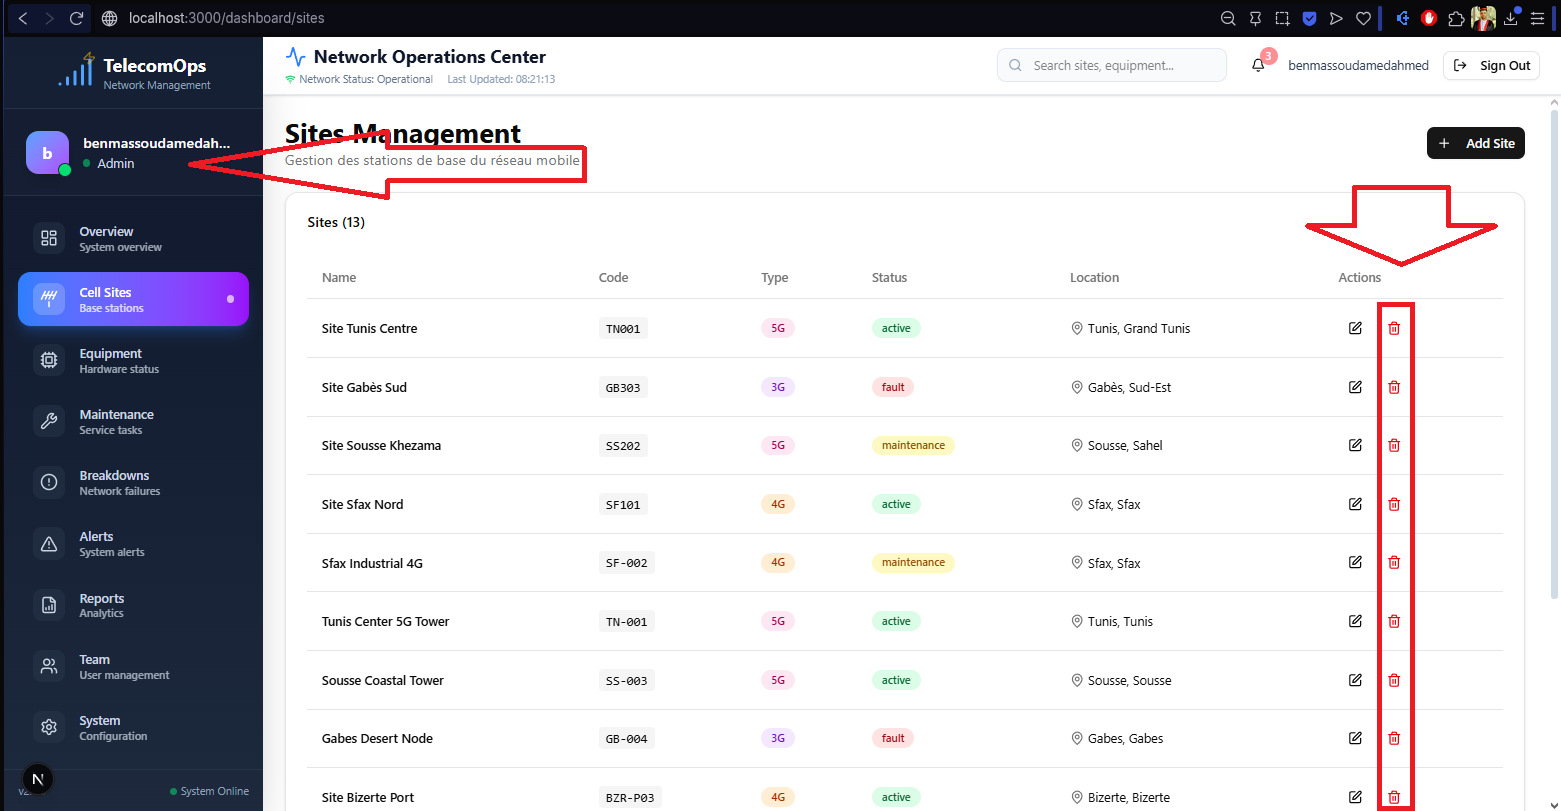
\includegraphics[width=0.85\linewidth]{img/chap_03/delete_site_modal.png}
    \caption{Delete Site Confirmation Modal}
    \label{fig:delete_site_modal}
\end{figure}

\subsection{User Profile Management}

Figure 3.11 illustrates the user profile management interface where users update personal information and change passwords securely.

\begin{figure}[H]
    \centering
    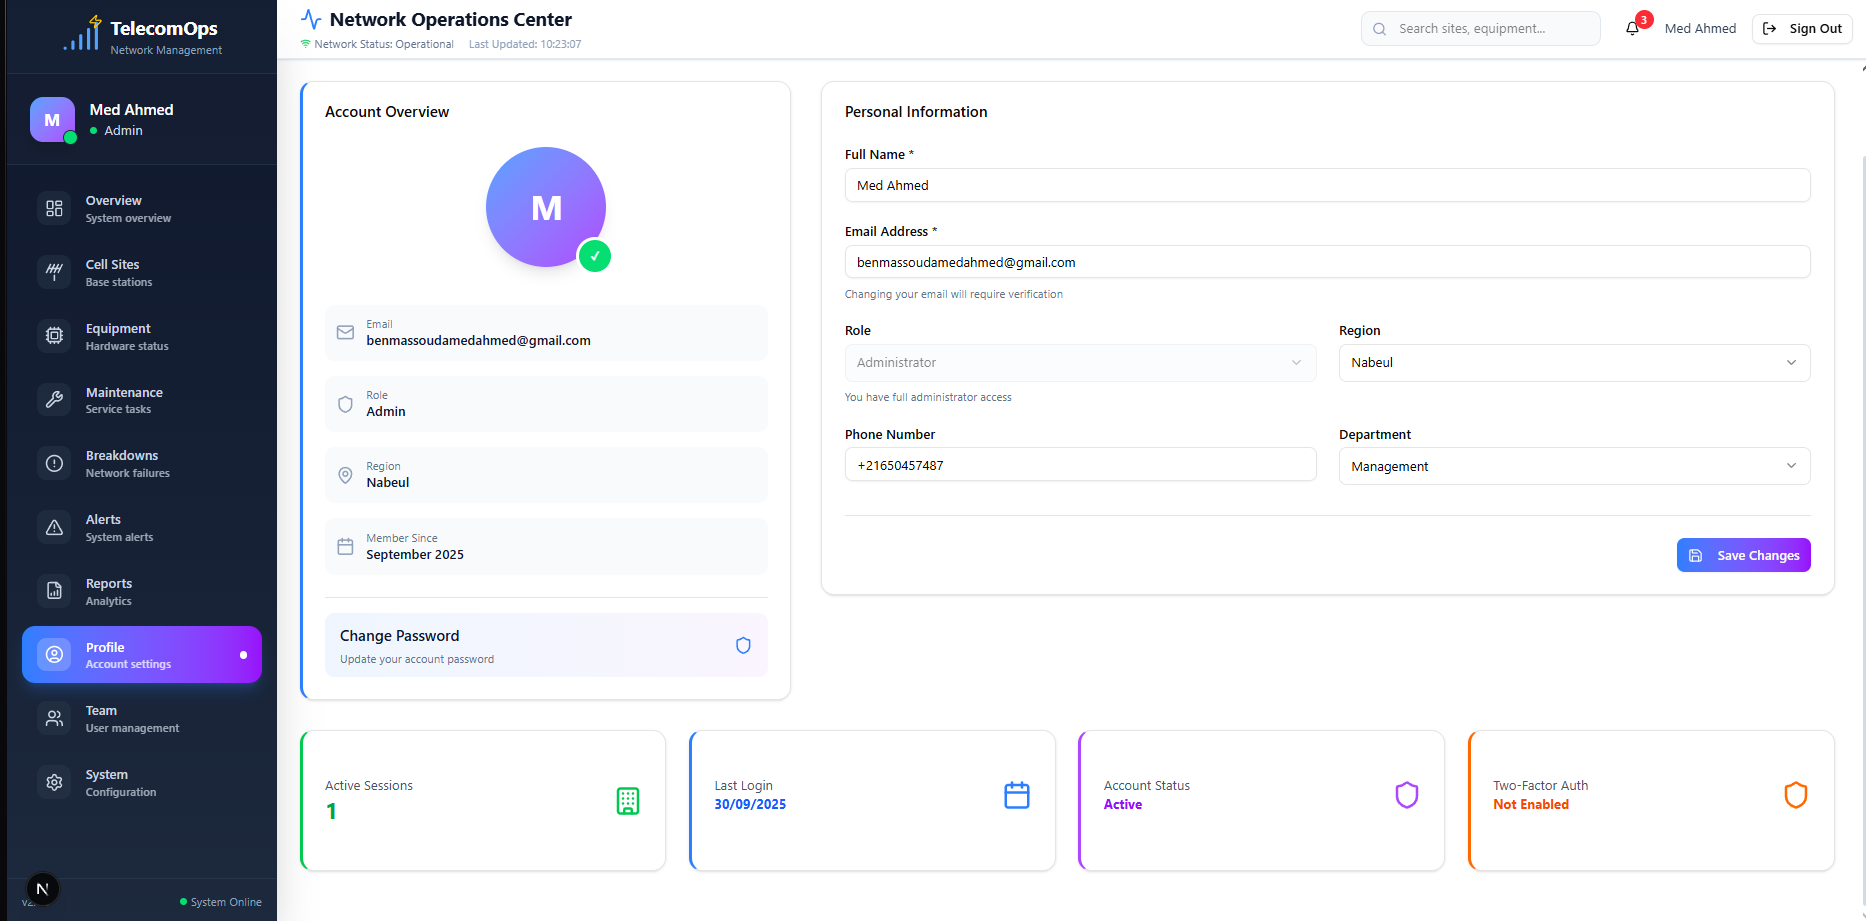
\includegraphics[width=0.85\linewidth]{img/chap_03/profile_management.png}
    \caption{User Profile Management Interface}
    \label{fig:profile_management}
\end{figure}

\section{Technical Challenges and Solutions}

Sprint 1 implementation encountered several technical challenges requiring careful analysis and innovative solutions.

\subsection{Row Level Security Configuration}

Implementing comprehensive Row Level Security policies presented significant complexity. Initial configurations caused permission errors preventing legitimate operations. Resolution involved developing granular RLS policies distinguishing between user roles while maintaining security. Policies now properly enforce that administrators, engineers, and managers can create and edit sites, while all authenticated users view site information. The enhanced Manager role required specific policies granting create and update permissions while restricting delete operations to administrators only.

\subsection{Real-time Data Synchronization}

Ensuring data consistency across multiple users accessing sites simultaneously required implementing Supabase's real-time subscriptions. When one user creates or updates sites, all connected users see changes immediately without page refresh. This was achieved through WebSocket connections managed by Supabase's real-time engine, implementing the real-time capabilities specified in Chapter 2's application layer architecture.

\subsection{Session Management and Security}

Implementing secure session management with automatic timeout required careful JWT token handling. The solution implements 30-minute inactivity timeout with automatic token refresh, secure token storage in memory rather than localStorage preventing XSS attacks, and session validation on each protected route access. This addresses NFR-004 authentication security requirements from Chapter 2.

\section{Testing and Validation}

Sprint 1 underwent comprehensive testing ensuring reliability, security, and proper role-based access control as specified in Chapter 2's success criteria.

\subsection{Authentication Security Testing}

Testing validated authentication bypass prevention, session management, and password security. All tests confirmed Supabase authentication properly protects against SQL injection, cross-site scripting, and brute force attacks. Failed login attempts trigger appropriate delays, and account lockout activates after five consecutive failures.

\subsection{Role-Based Access Testing}

Each user role was tested verifying appropriate access levels. Table 3.3 summarizes role testing results.

\begin{table}[H]
\centering
\small
\begin{tabular}{|l|c|c|c|c|}
\hline
\textbf{Operation} & \textbf{Admin} & \textbf{Engineer} & \textbf{Technician} & \textbf{Manager} \\
\hline
View Sites & Allowed & Allowed & Allowed & Allowed \\
\hline
Create Site & Allowed & Allowed & Denied & Allowed \\
\hline
Edit Site & Allowed & Allowed & Denied & Allowed (Status Only) \\
\hline
Delete Site & Allowed & Denied & Denied & Denied \\
\hline
Manage Users & Allowed & Denied & Denied & Denied \\
\hline
\end{tabular}
\caption{Role-Based Access Testing Results}
\label{tab:role_testing}
\end{table}

All unauthorized operations were properly blocked by Row Level Security policies, confirming the security architecture's effectiveness.

\subsection{Site Management Functional Testing}

Complete CRUD operations were validated: site creation with unique code enforcement preventing duplicates, site editing with proper field validation ensuring data integrity, site deletion restricted to administrators with referential integrity checking, and real-time list updates across multiple user sessions confirming WebSocket functionality. All tests passed successfully, meeting the success criteria defined in Chapter 2, Section 2.5.2.

\subsection{Performance Testing}

Performance testing validated NFR-001 requirements from Chapter 2. Page load times averaged 2.1 seconds (target: under 3 seconds), API response times averaged 280ms (target: under 500ms), and real-time updates propagated within 1.5 seconds (target: within 2 seconds). All performance metrics exceeded established targets.

\section{Sprint Review and Retrospective}

Sprint 1 review with stakeholders confirmed successful delivery of all committed user stories. Stakeholders approved the authentication system's security implementation, site management interface's usability, and role-based access control's accurate reflection of organizational structure. User acceptance testing across all four user roles validated the implementation meets operational requirements.

The sprint retrospective identified several positive outcomes: Supabase integration accelerated development by providing authentication infrastructure without custom backend development; TypeScript type safety prevented numerous potential runtime errors during development; and Next.js server-side rendering provided excellent initial page load performance. Areas for improvement include earlier stakeholder involvement in interface design and more comprehensive integration testing earlier in the sprint.

\section{Conclusion}

Sprint 1 successfully established the foundational authentication infrastructure and site management capabilities essential for TelecomOps. The implementation delivered secure user authentication using Supabase Auth, comprehensive site management functionality with CRUD operations split into three distinct user stories (US-003A, US-003B, US-003C) for precise permission management, role-based access control enforced through Row Level Security, and user profile management with password change capabilities.

The sprint addressed all high-priority user stories from Chapter 2's product backlog, implementing the authentication and presentation layers specified in the system architecture. The enhanced Manager role provides appropriate operational oversight capabilities while maintaining security boundaries, reflecting the stakeholder analysis from Chapter 2.

Quality metrics exceeded established targets with successful user acceptance testing across all user roles, performance metrics surpassing NFR-001 requirements, and comprehensive security validation confirming the multi-layer security architecture's effectiveness. The implementation demonstrates effective integration of Next.js, TypeScript, and Supabase while addressing real-world telecommunications operational requirements.

Sprint 1 establishes a robust foundation for subsequent development. The authentication infrastructure enables all future features requiring user identification and authorization. The site management foundation provides the core entity upon which equipment inventory, interventions, and monitoring features will build in subsequent sprints.

The next chapter presents Sprint 2, titled "Equipment Monitoring and Inventory Management," which extends the site management foundation with comprehensive equipment tracking, lifecycle management, and maintenance scheduling capabilities, addressing user stories US-005A-C, US-006, and US-016A-B from the product backlog.
        \clearpage
        
        \newpage

\chapter{Sprint 2: Equipment Monitoring and Inventory}

\cfoot{\thepage}

\parindent=0.5in
\onehalfspacing

\section{Introduction}

Following the successful completion of Sprint 1 which established authentication and site management foundations, we now focus on Sprint 2 titled "Equipment Monitoring and Inventory". This sprint concentrates on the design and implementation of equipment tracking and inventory management modules essential for comprehensive telecommunications network asset management.

The second sprint extends site management capabilities by introducing detailed equipment inventory tracking, enabling network engineers and technicians to monitor all network hardware across telecommunications sites. This includes managing equipment lifecycle, tracking status changes, and maintaining accurate records of installation and warranty information critical for proactive network maintenance.

\section{Sprint Backlog}

During the sprint planning meeting, we discussed with the Scrum Master the tasks required in this sprint, presented in Table 4.1 below.

\begin{table}[H]
\centering
\small
\begin{tabular}{|p{2.5cm}|p{4cm}|p{2.8cm}|c|c|}
\hline
\textbf{Functionality} & \textbf{User Story} & \textbf{Tasks} & \textbf{Complexity} & \textbf{Est.} \\
\hline
Equipment Registration & 
As admin and engineer, I can add new equipment with serial numbers.
& 
Equipment creation
Serial validation
Testing
& 
Med
Hard  
Med
& 
5
5
3 \\
\hline
Status Tracking & 
As technician, engineer, and admin, I can update equipment status.
& 
Status management
Status interfaces
Testing
& 
Med
Easy
Med
& 
4
2
3 \\
\hline
Equipment Inventory & 
As all users, I can view equipment. As admin and engineer, I can edit.
& 
Equipment CRUD
Equipment interfaces
Testing
& 
Med
Med
Hard
& 
5
4
5 \\
\hline
Equipment Statistics & 
As manager, engineer, and admin, I can view equipment statistics.
& 
Statistics calculation
Dashboard cards
Testing
& 
Med
Easy
Med
& 
4
2
3 \\
\hline
\end{tabular}
\caption{Sprint 2 Backlog}
\label{tab:sprint2_backlog}
\end{table}

\section{Class Diagram}

The class diagram for this sprint focuses on equipment management and relationships with telecommunications sites.

\begin{figure}[H]
    \centering
    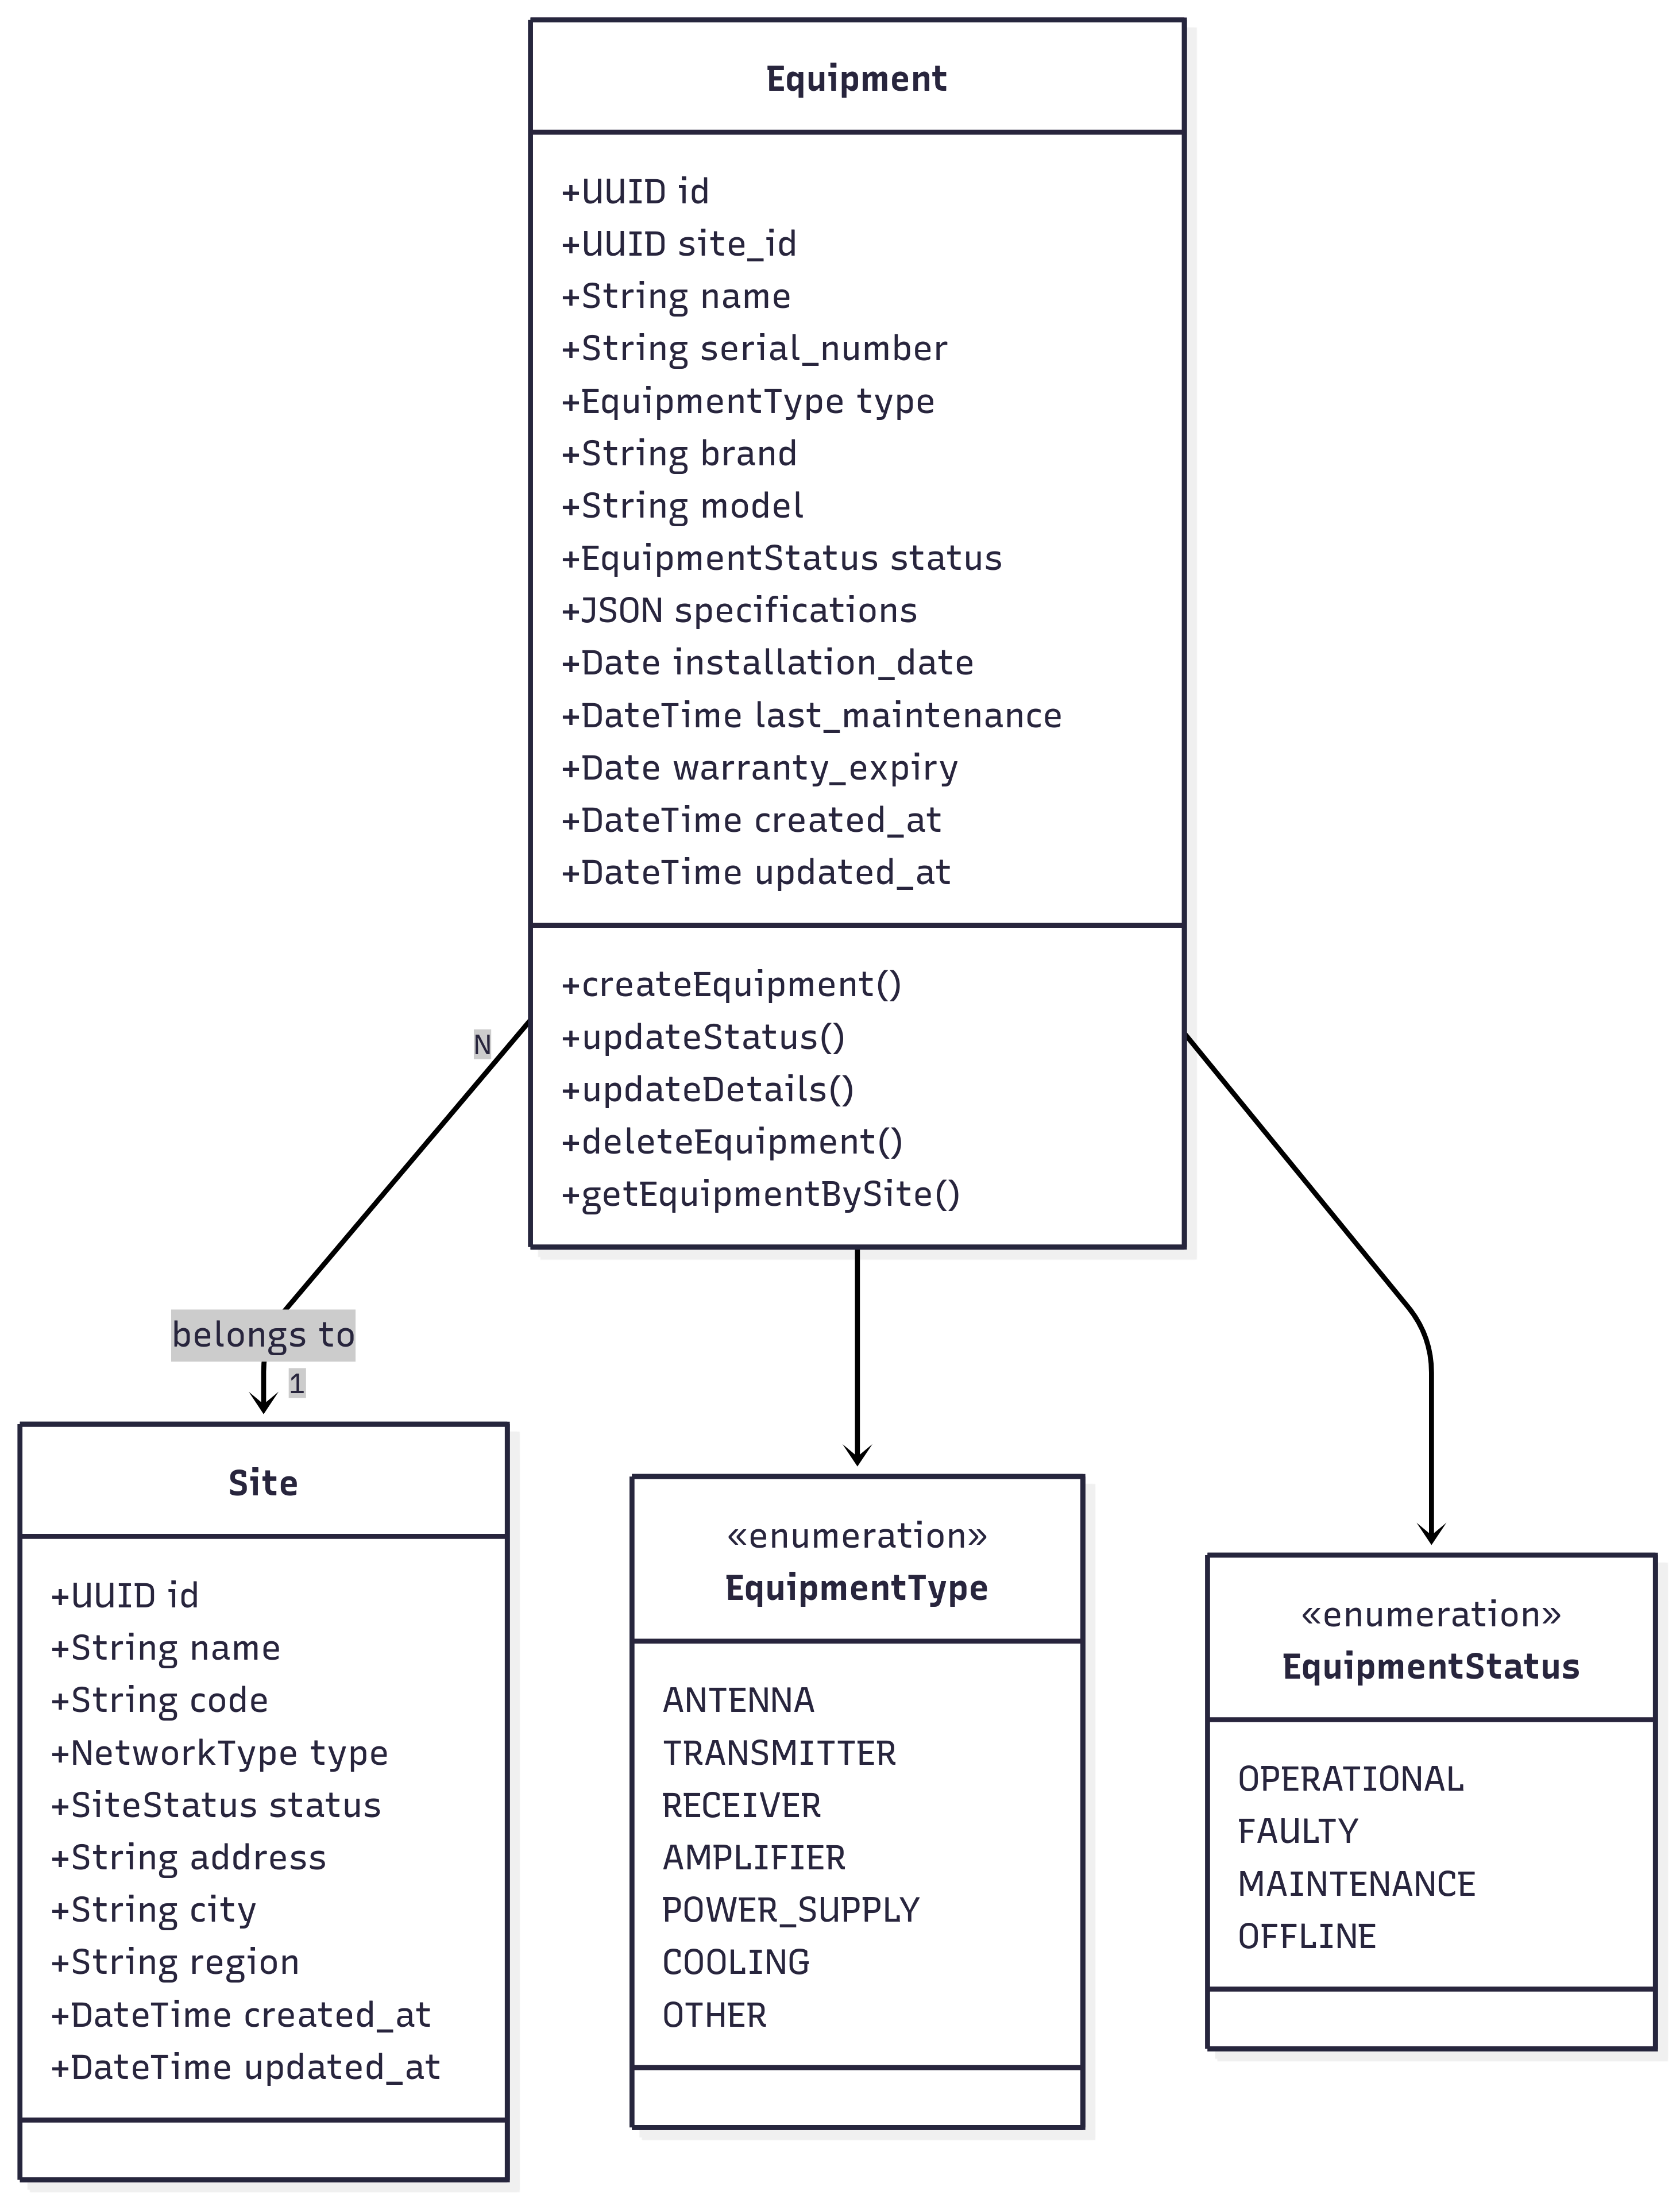
\includegraphics[width=0.8\linewidth]{img/chap_04/equipment_class_diagram.png}
    \caption{Class Diagram "Equipment Monitoring and Inventory"}
    \label{fig:class_diagram_sprint2}
\end{figure}

The diagram illustrates the relationship between \texttt{Equipment} and \texttt{Sites}. The \texttt{Equipment} class maintains unique serial numbers, equipment type classifications, operational status, brand and model information, and warranty details. The \texttt{EquipmentType} and \texttt{EquipmentStatus} enumerations ensure controlled values. The many-to-one relationship ensures every equipment item is associated with a specific network location.

\section{Use Case Diagram}

The use case diagram shows actors and their hierarchical interactions with the equipment management system.

\begin{figure}[H]
    \centering
    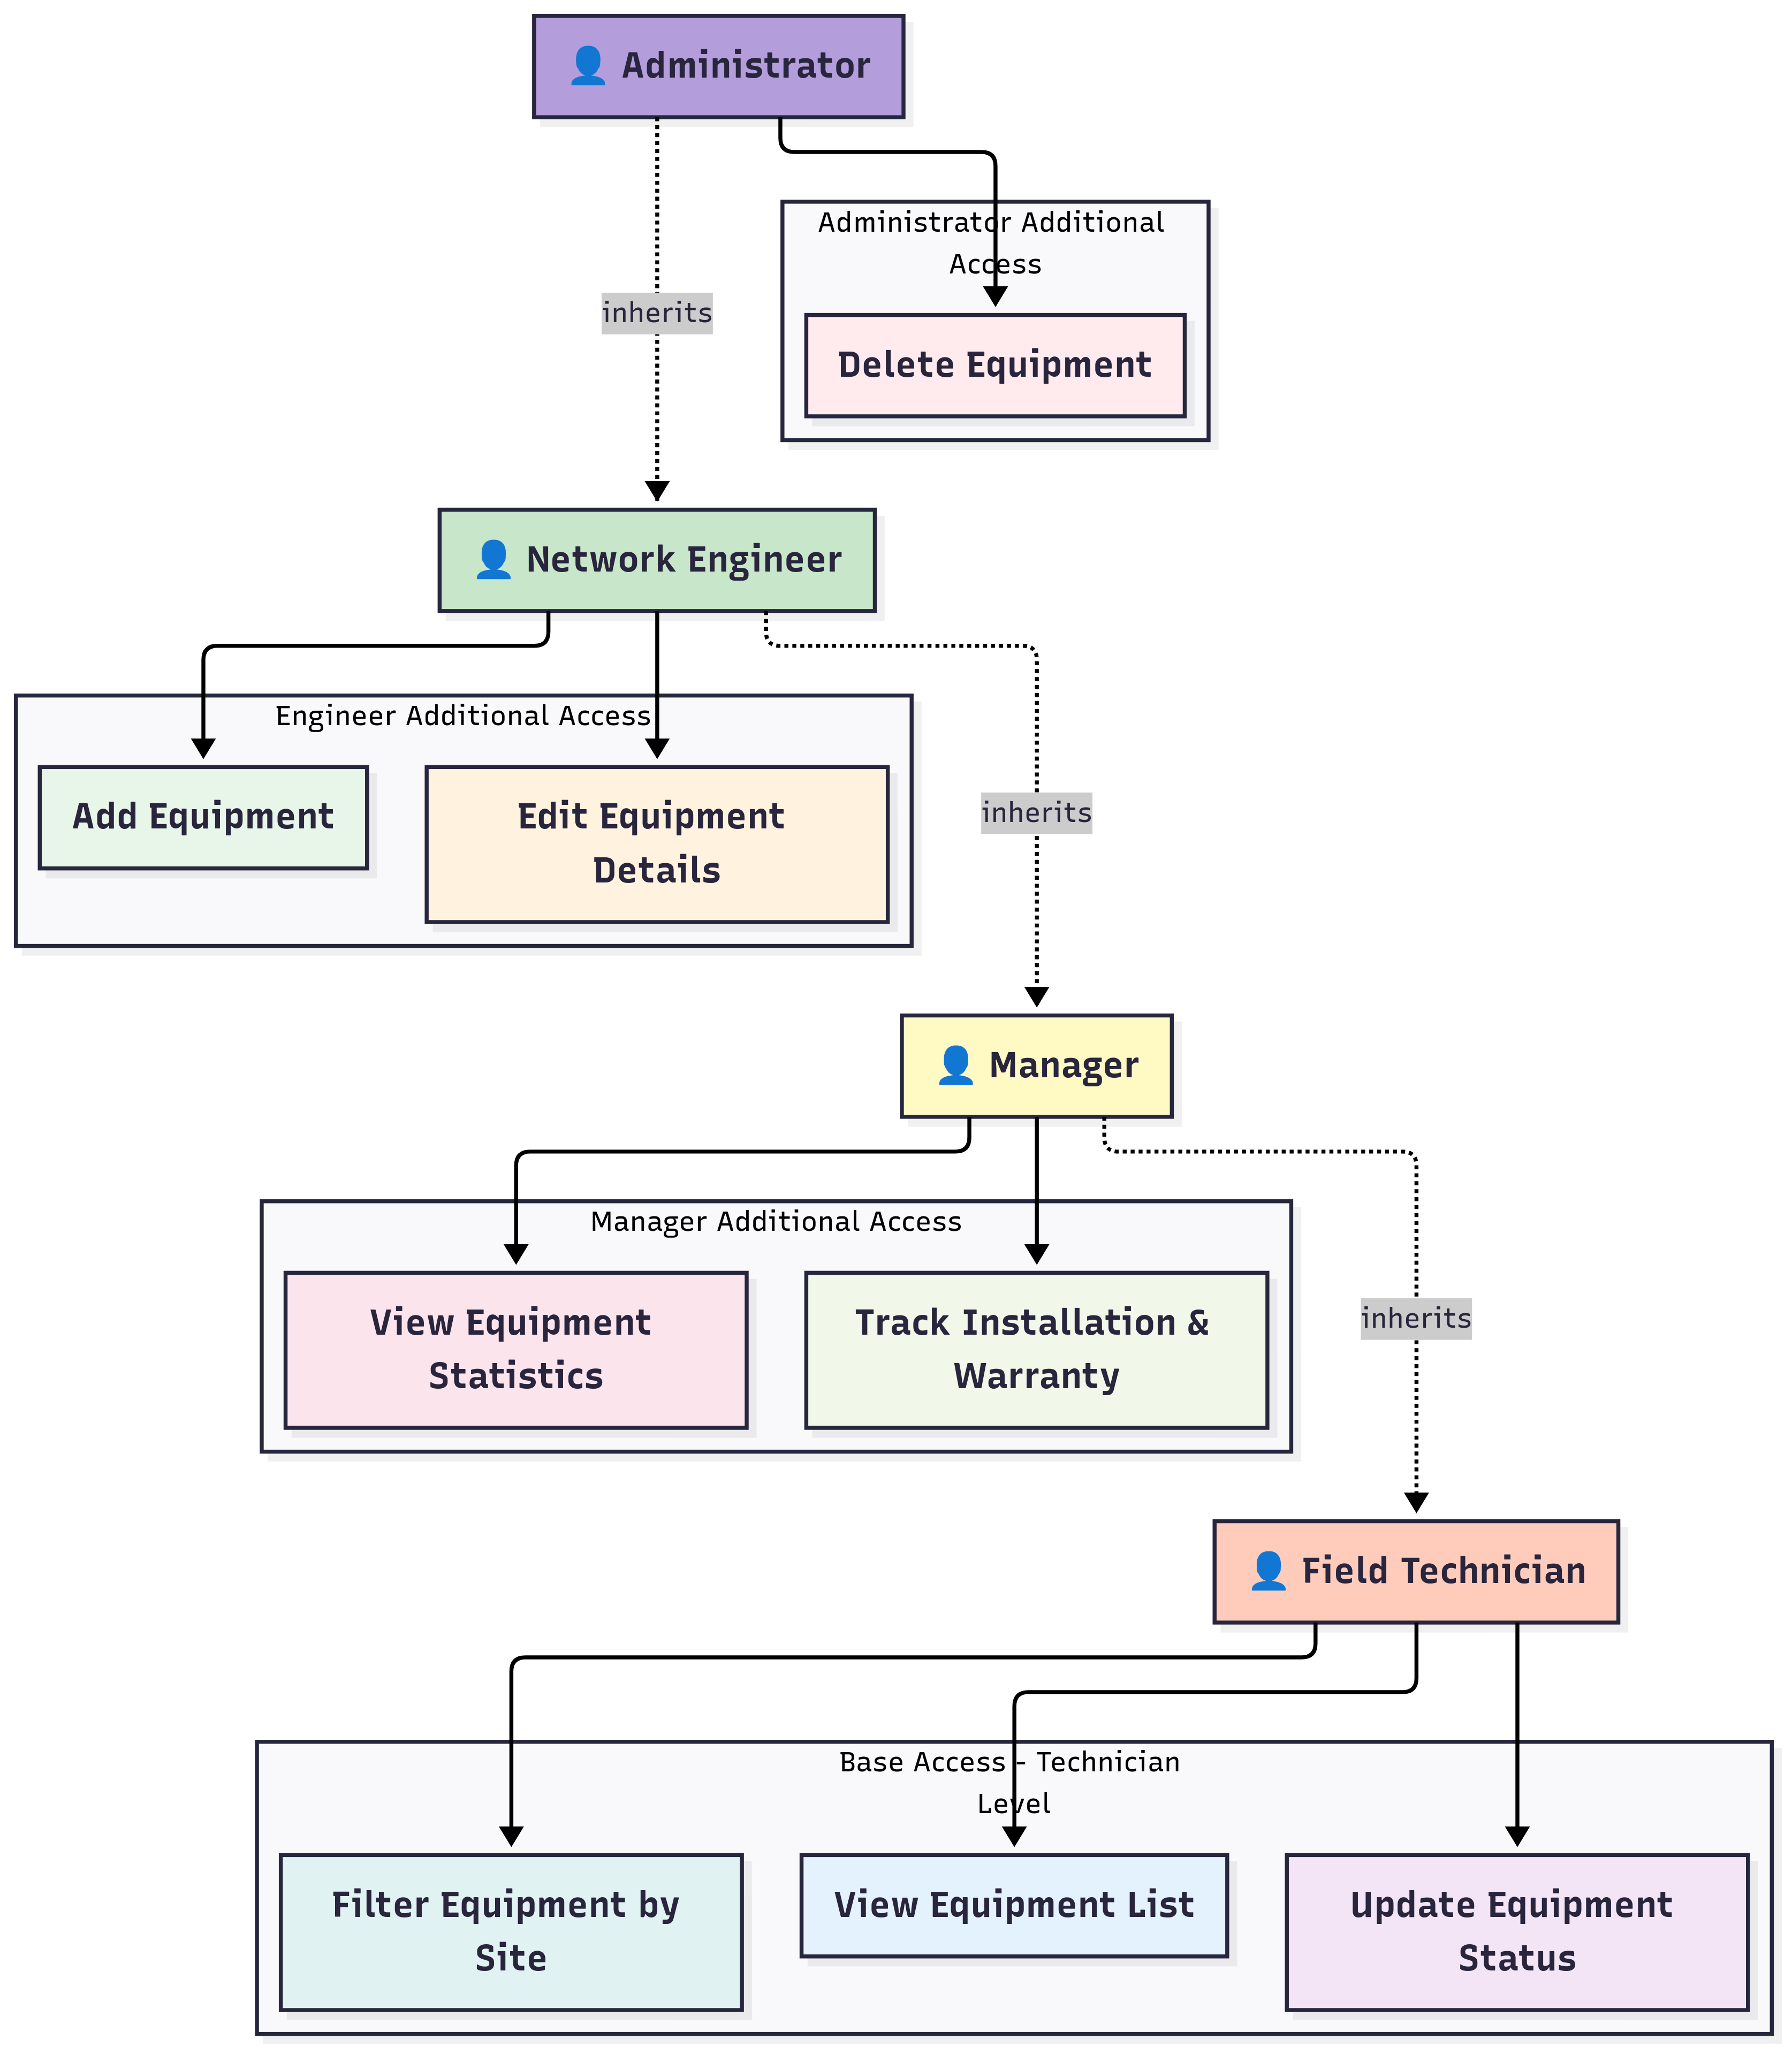
\includegraphics[width=0.75\linewidth]{img/chap_04/equipment_usecase_diagram.png}
    \caption{Use Case Diagram "Equipment Monitoring and Inventory"}
    \label{fig:use_case_diagram_sprint2}
\end{figure}

The diagram implements an inheritance hierarchy across four actor types. Field Technicians have base access (view, update status, filter by site). Managers inherit technician permissions plus statistics and warranty tracking. Network Engineers inherit manager permissions plus add and edit equipment. Administrators inherit all engineer permissions plus exclusive deletion rights.

\begin{table}[H]
\centering
\caption{Equipment Management Permissions by Role}
\label{tab:equipment-permissions}
\small
\begin{tabular}{|p{3.5cm}|c|c|c|c|}
\hline
\textbf{Use Case} & \textbf{Tech} & \textbf{Mgr} & \textbf{Eng} & \textbf{Admin} \\
\hline
View Equipment List & Yes & Yes & Yes & Yes \\
\hline
Update Equipment Status & Yes & Yes & Yes & Yes \\
\hline
Filter Equipment by Site & Yes & Yes & Yes & Yes \\
\hline
View Equipment Statistics & No & Yes & Yes & Yes \\
\hline
Track Installation \& Warranty & No & Yes & Yes & Yes \\
\hline
Add Equipment & No & No & Yes & Yes \\
\hline
Edit Equipment Details & No & No & Yes & Yes \\
\hline
Delete Equipment & No & No & No & Yes \\
\hline
\end{tabular}
\end{table}

Table 4.2 shows the permission matrix. Technicians have three capabilities, managers have five, engineers have seven, and administrators have eight (all capabilities).

\subsection{Use Case Description: Add Equipment}

Table 4.3 provides detailed information on the "Add Equipment" use case.

\begin{table}[H]
\centering
\small
\begin{tabular}{|p{3cm}|p{7.5cm}|}
\hline
\textbf{Use Case} & Add Equipment \\
\hline
\textbf{Primary Actors} & Administrator, Network Engineer \\
\hline
\textbf{Pre-condition} & User authenticated with appropriate role; active site exists \\
\hline
\textbf{Post-condition} & Equipment created in database with operational status \\
\hline
\textbf{Main Scenario} & 
1. User accesses equipment management interface.
2. User clicks "Add Equipment" button.
3. User fills form (name, serial, type, brand, site).
4. User submits form.
5. System validates fields and serial uniqueness.
6. System verifies permissions via RLS.
7. System creates equipment record.
8. System updates equipment list.
\\
\hline
\textbf{Exception Scenarios} & 
Error message if missing data, duplicate serial, invalid type, insufficient permissions, or connection problems.
\\
\hline
\end{tabular}
\caption{Use Case: Add Equipment}
\label{tab:add_equipment_usecase}
\end{table}

\section{Sequence Diagrams}

Sequence diagrams provide detailed explanations of the main processes in this sprint.

\subsection{Add Equipment Sequence Diagram}

\begin{figure}[H]
    \centering
    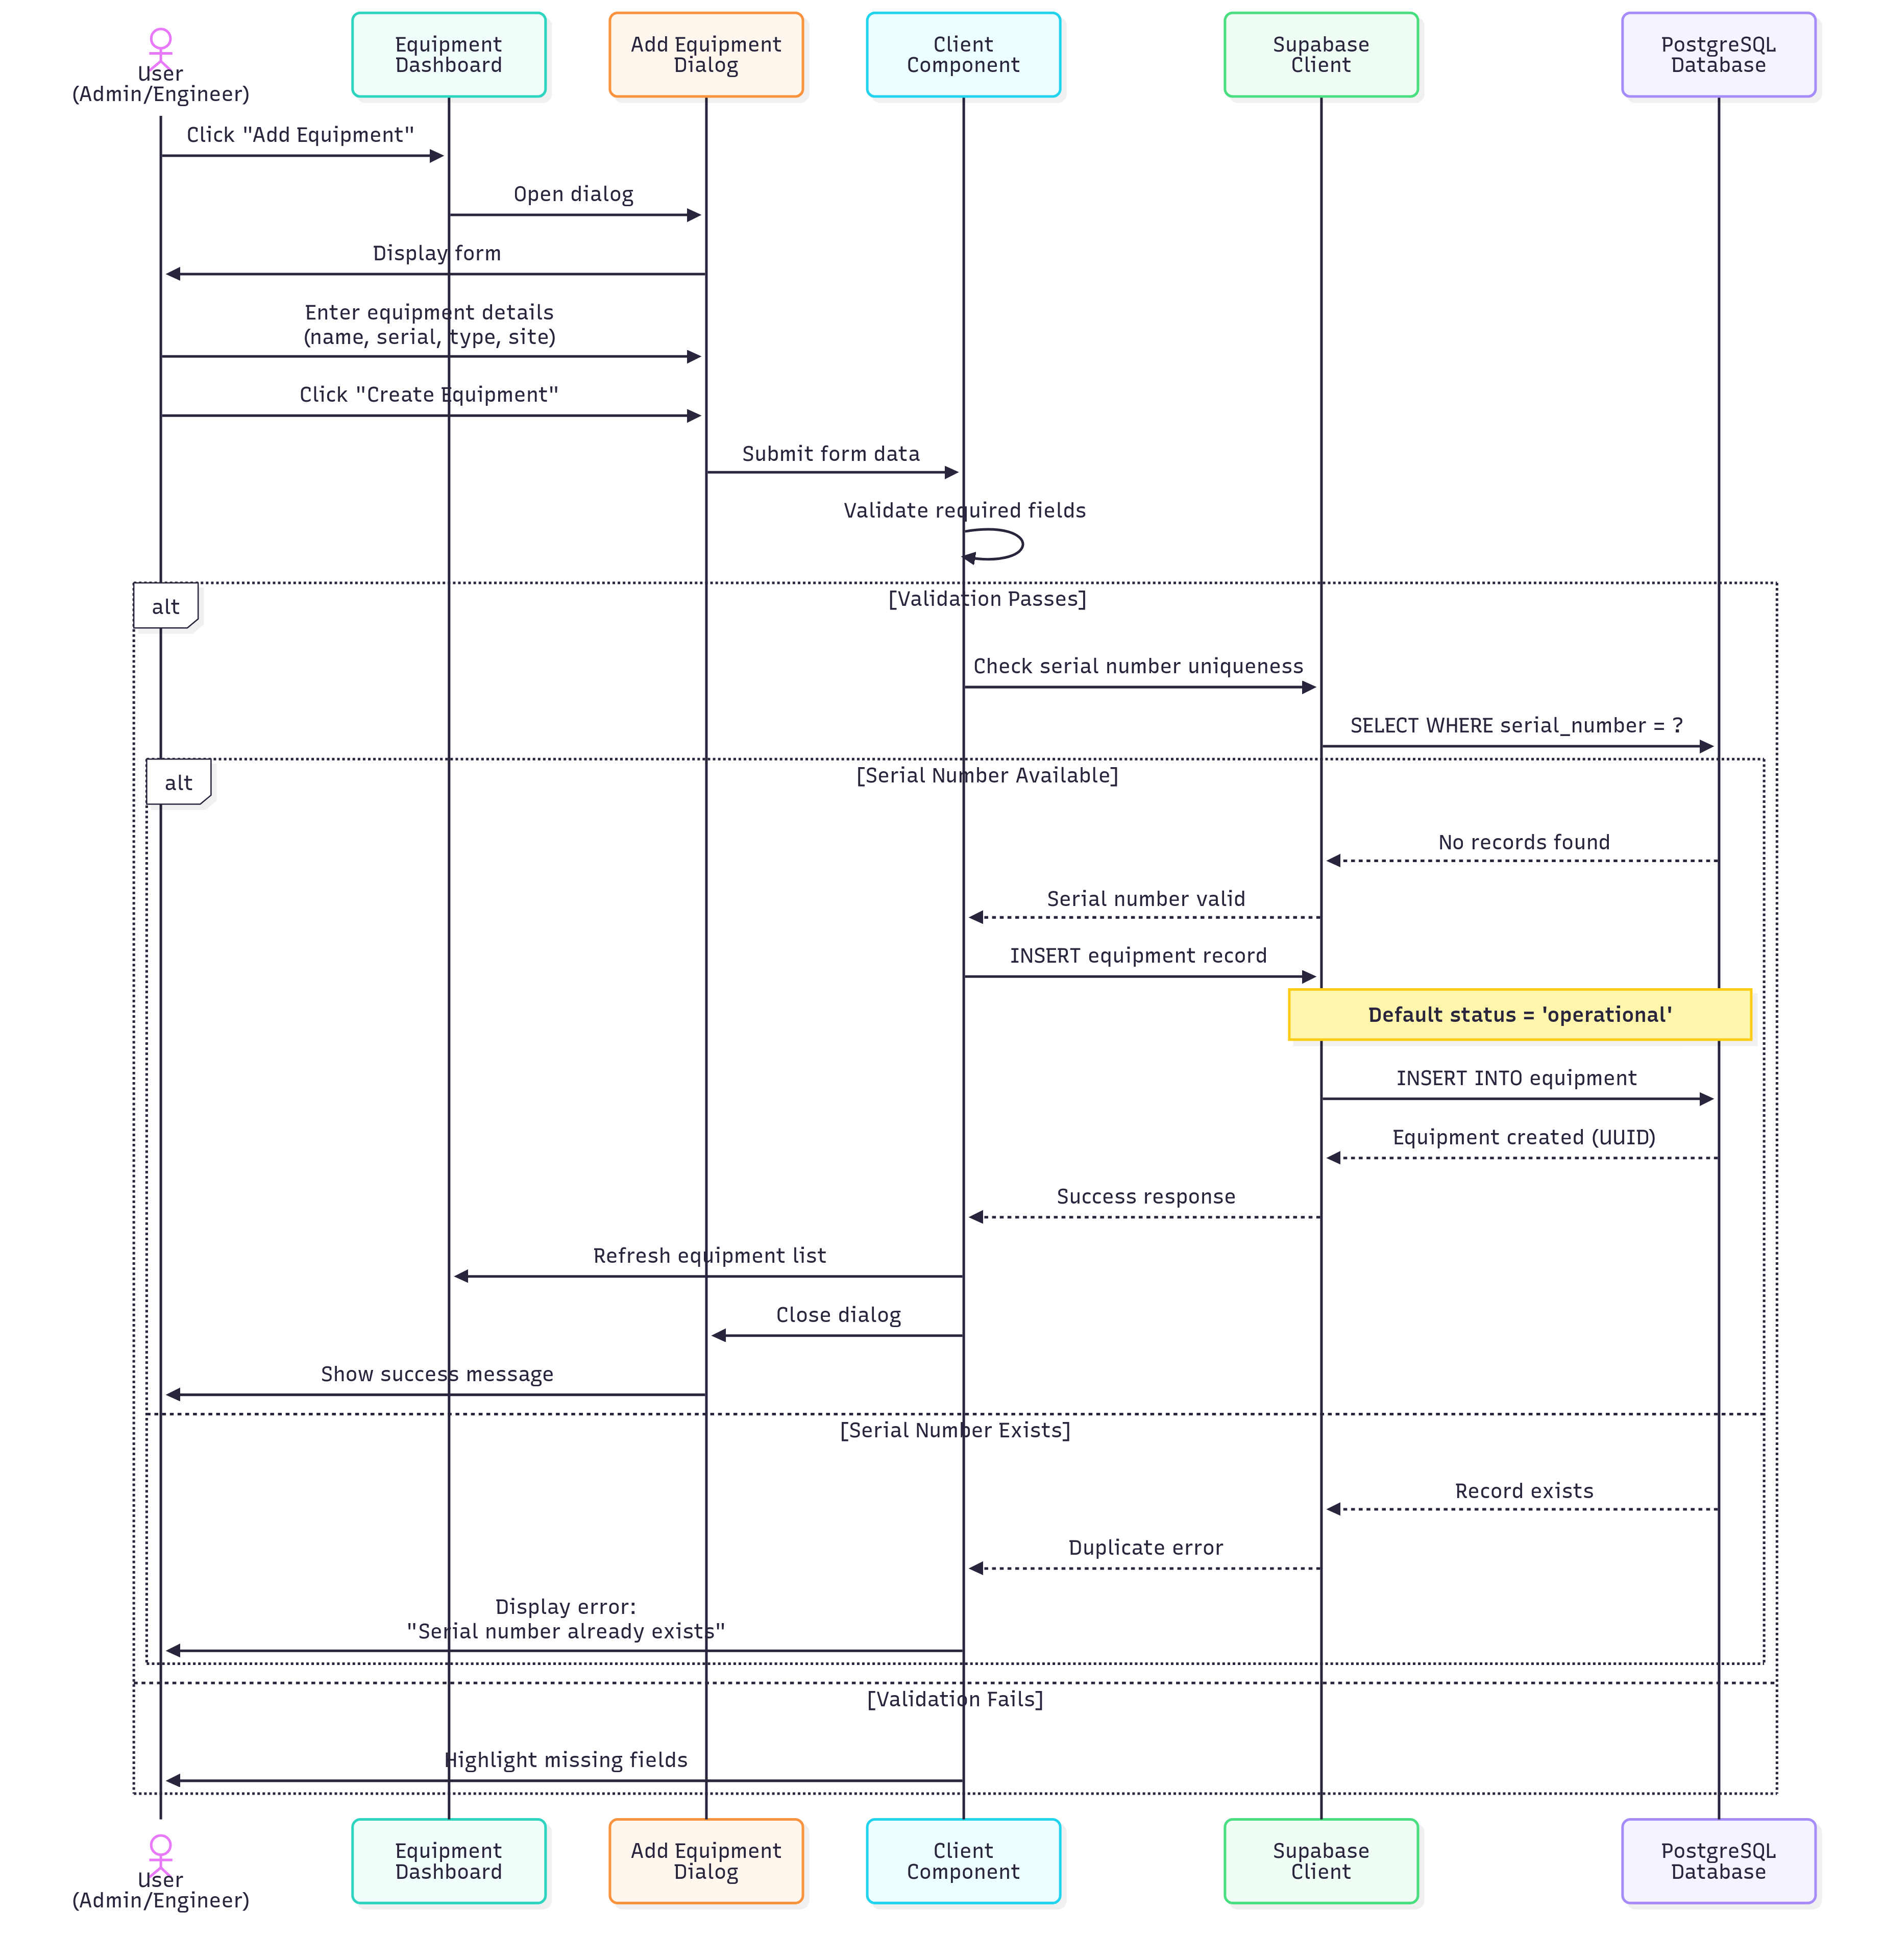
\includegraphics[width=0.85\linewidth]{img/chap_04/add_equipment_sequence.png}
    \caption{Sequence Diagram "Add Equipment"}
    \label{fig:sequence_add_equipment}
\end{figure}

The add equipment sequence diagram demonstrates the workflow for registering new network equipment. An authorized user (Administrator or Engineer) accesses the interface and clicks "Add Equipment", displaying a creation modal. After entering required details (name, serial number, type, site), the user submits the form. The system validates fields and checks serial number uniqueness through database query. If available, the system creates the equipment record with "operational" status via \texttt{supabase.from('equipment').insert()}. Upon success, the equipment list updates in real-time and displays confirmation. Duplicate serial numbers trigger error messages.

\subsection{Edit Equipment Status Sequence Diagram}

\begin{figure}[H]
    \centering
    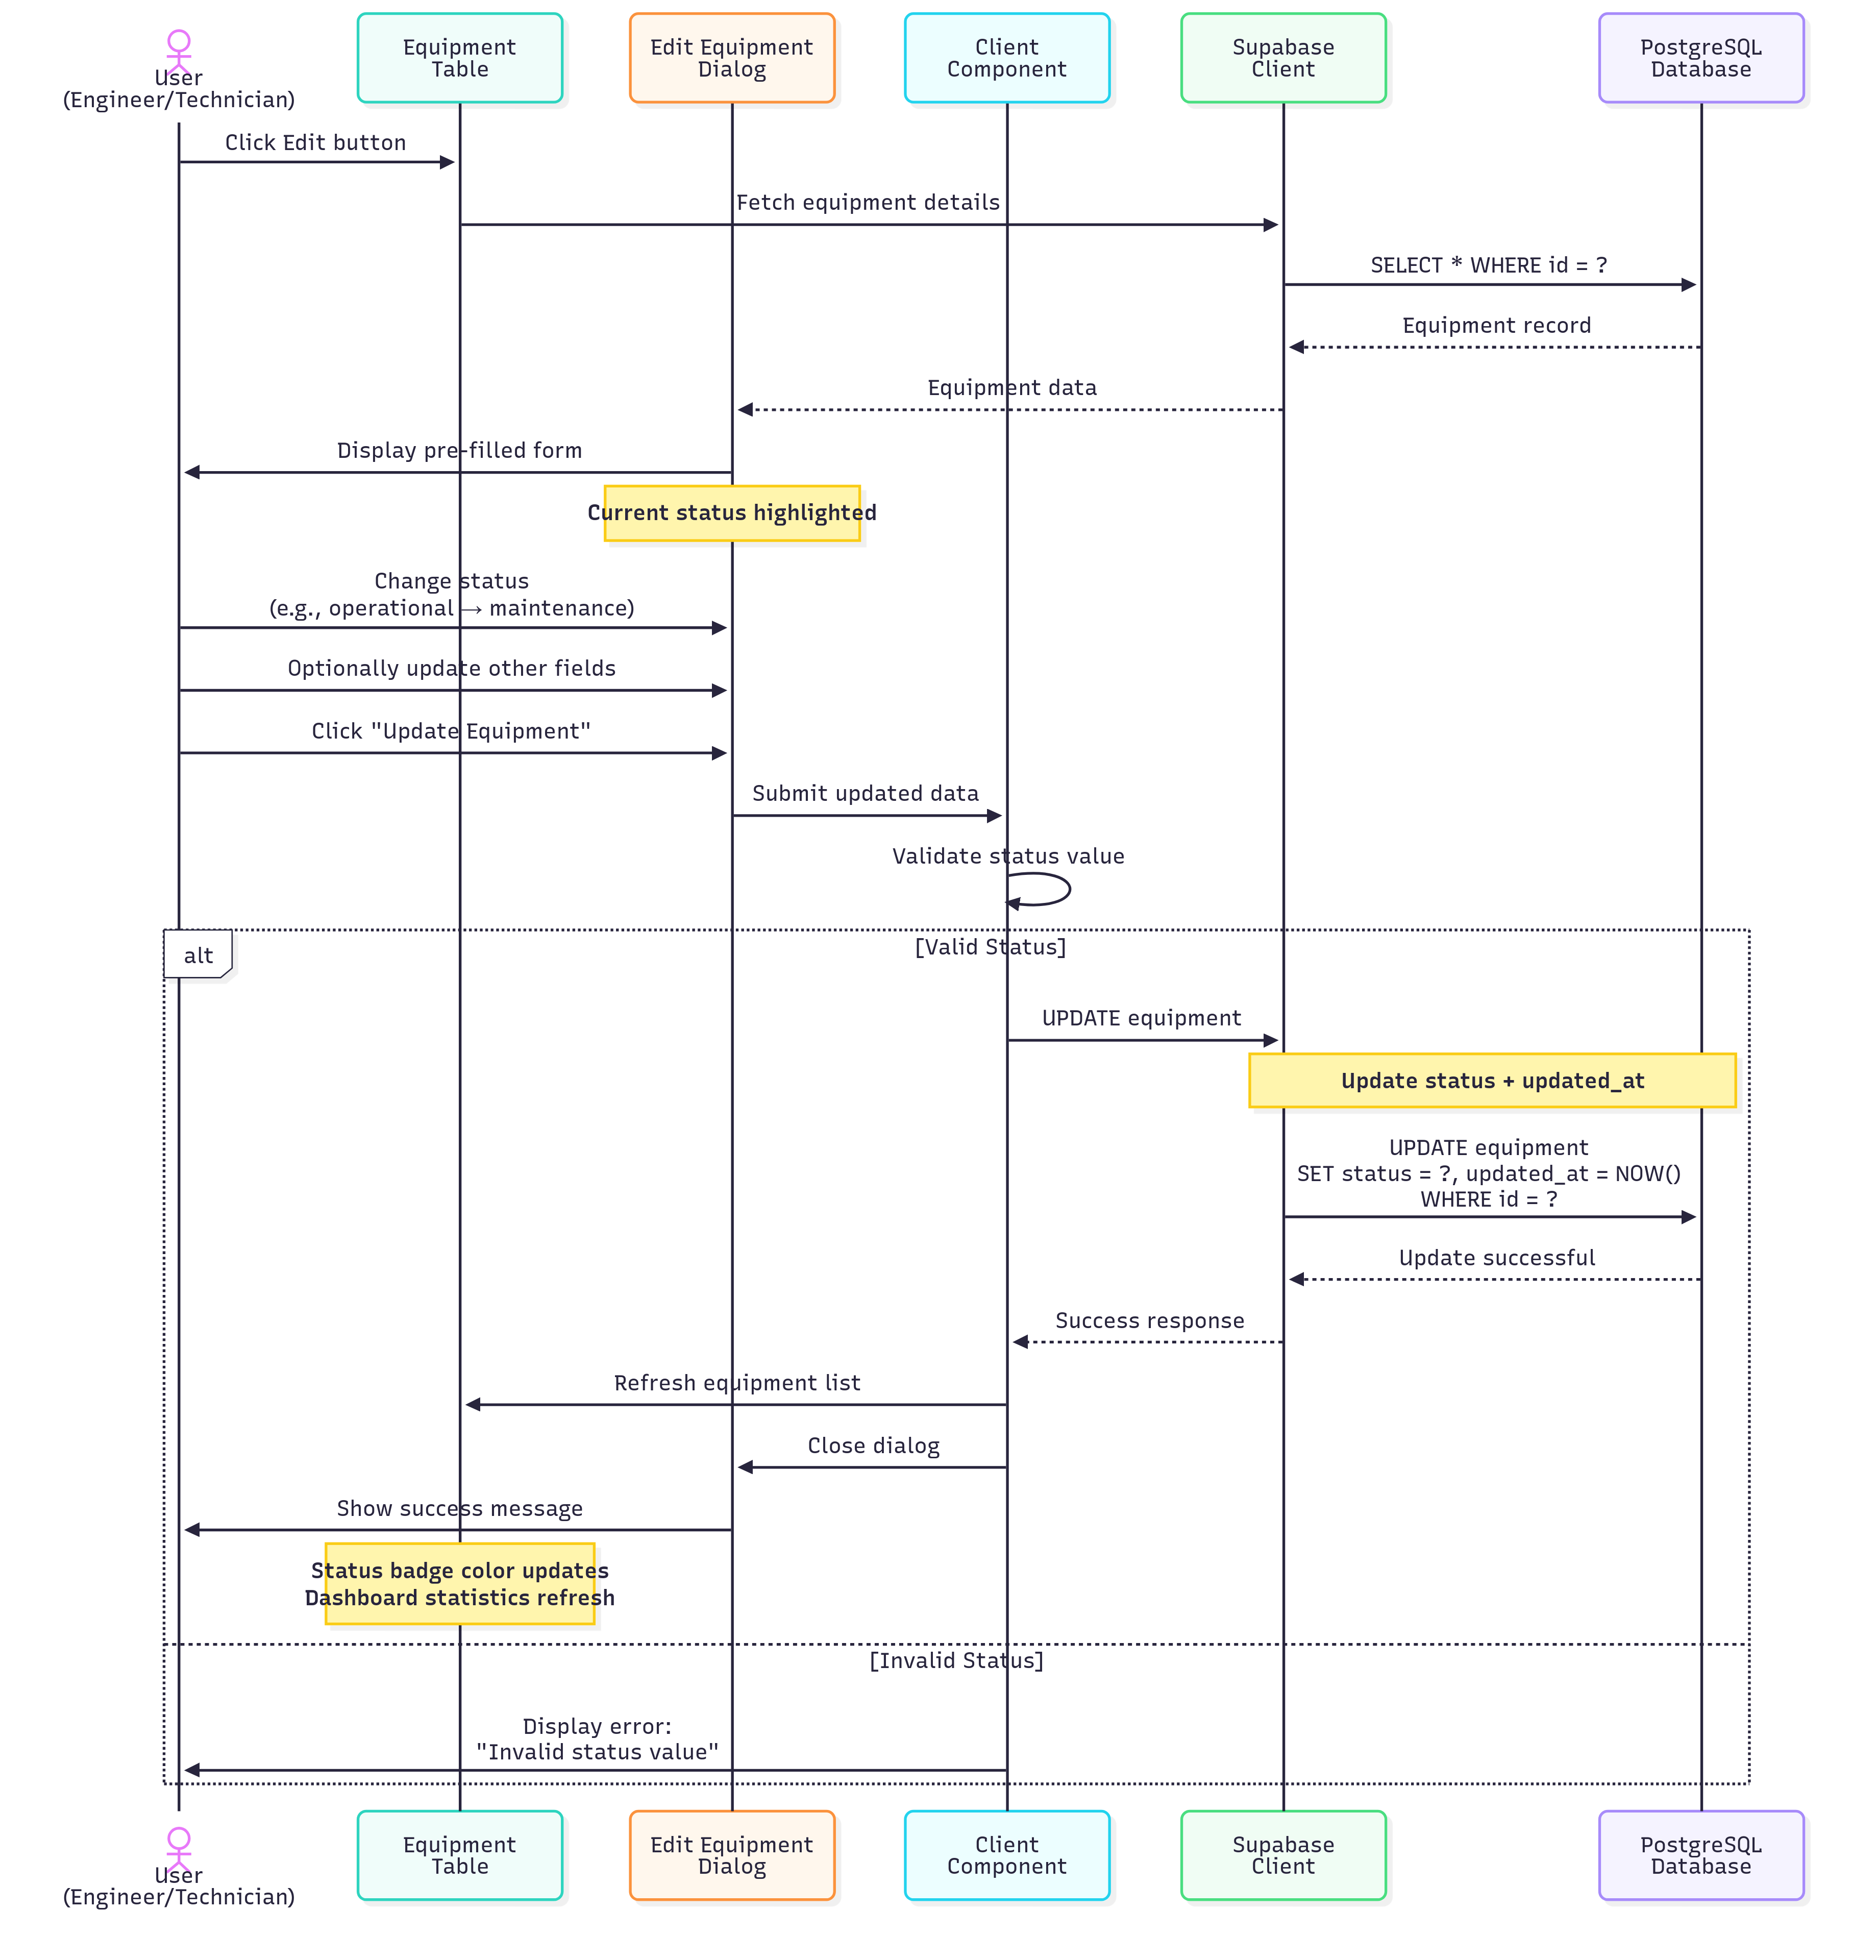
\includegraphics[width=0.85\linewidth]{img/chap_04/edit_equipment_status_sequence.png}
    \caption{Sequence Diagram "Edit Equipment Status"}
    \label{fig:sequence_edit_status}
\end{figure}

The edit status sequence diagram illustrates updating equipment operational state. When a user selects equipment and clicks edit, the system fetches current details including status. The dialog displays pre-filled fields with highlighted current status. The user modifies status (operational, faulty, maintenance, offline) and submits changes. The system validates the status value and sends an UPDATE request. The database verifies permissions through RLS and updates both status and \texttt{updated\_at} timestamp. Upon success, the equipment table refreshes across all sessions, the modal closes, and dashboard statistics recalculate automatically.

\section{Implementation}

Screenshots illustrating the interfaces developed during this sprint.

\subsection{Equipment Dashboard Interface}

\begin{figure}[H]
    \centering
    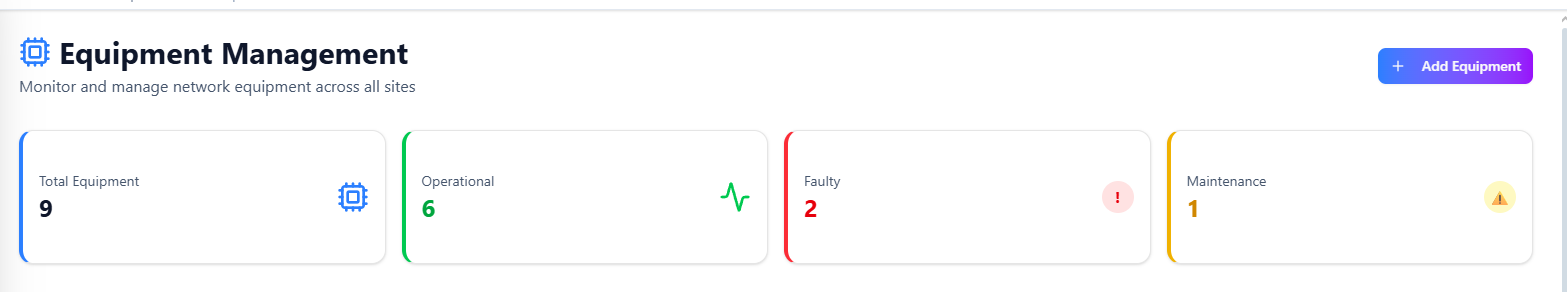
\includegraphics[width=0.8\linewidth]{img/chap_04/equipment_dashboard.png}
    \caption{Equipment Dashboard with Statistics}
    \label{fig:equipment_dashboard}
\end{figure}

The dashboard presents four statistical cards displaying real-time equipment counts by status with color-coded indicators (green: operational, red: faulty, yellow: maintenance, gray: offline).

\subsection{Equipment Management Interface}

\begin{figure}[H]
    \centering
    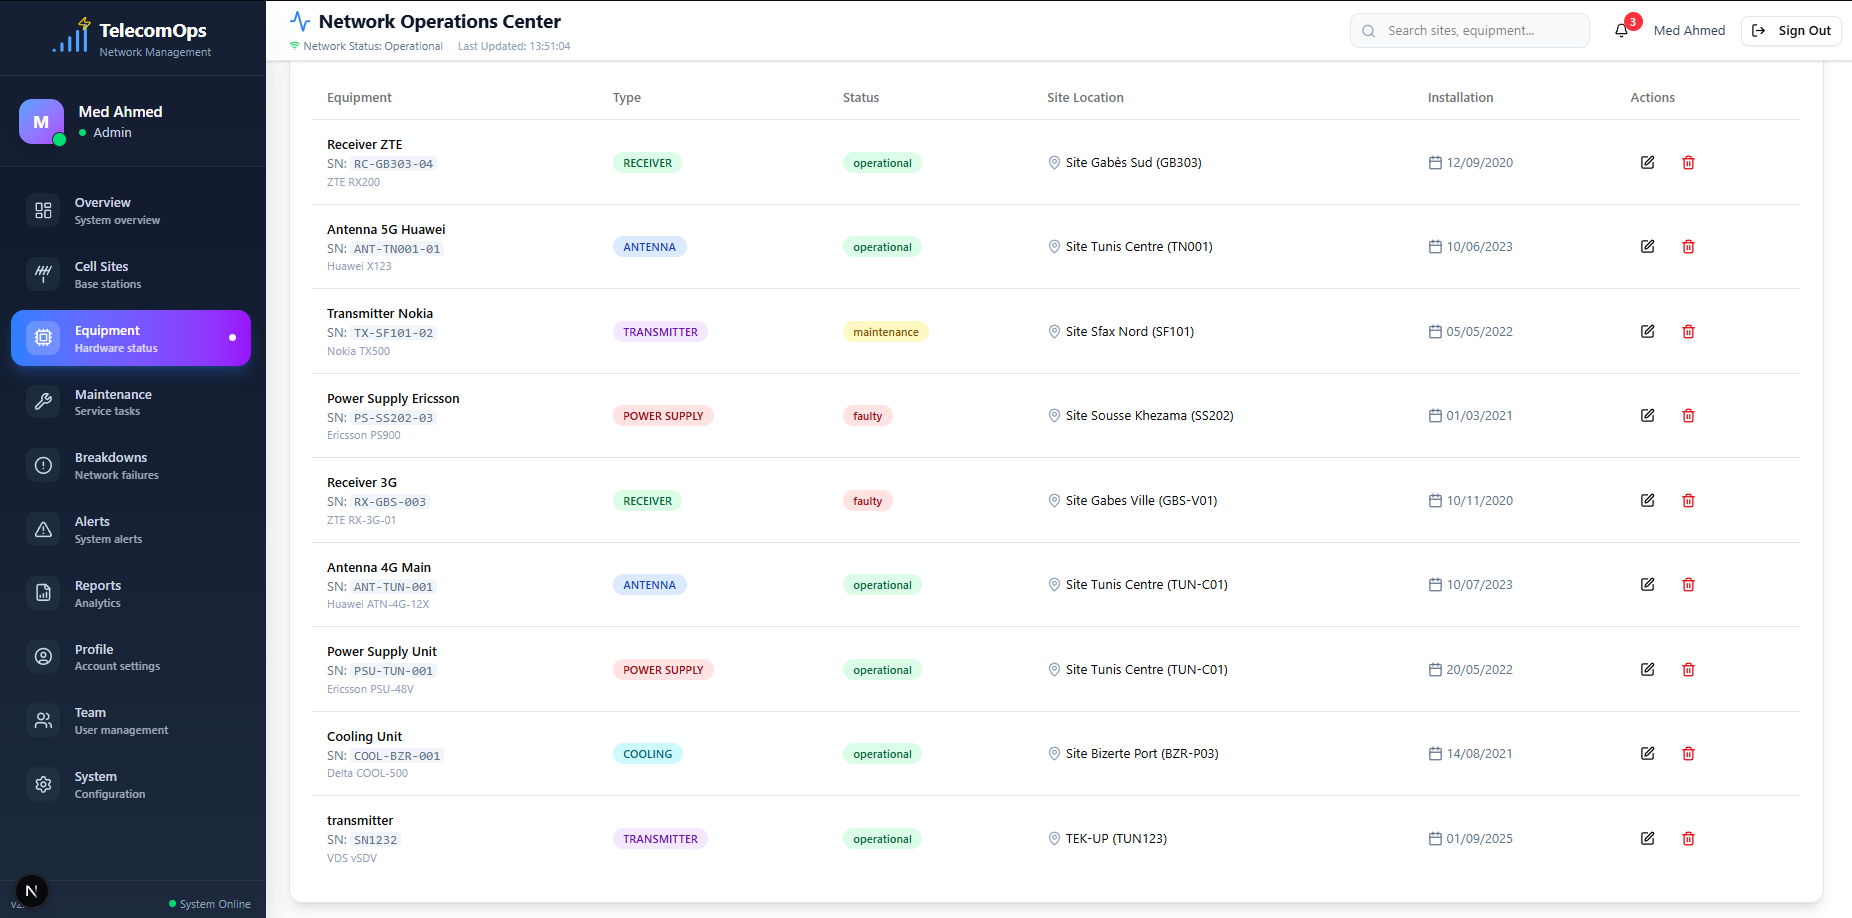
\includegraphics[width=0.8\linewidth]{img/chap_04/equipment_table.png}
    \caption{Equipment Inventory Table}
    \label{fig:equipment_table}
\end{figure}

The equipment table displays comprehensive information with columns for equipment name, serial number, type badge, status badge, site location, installation date, and action buttons.

\subsection{Equipment Management Modals}

\begin{figure}[H]
    \centering
    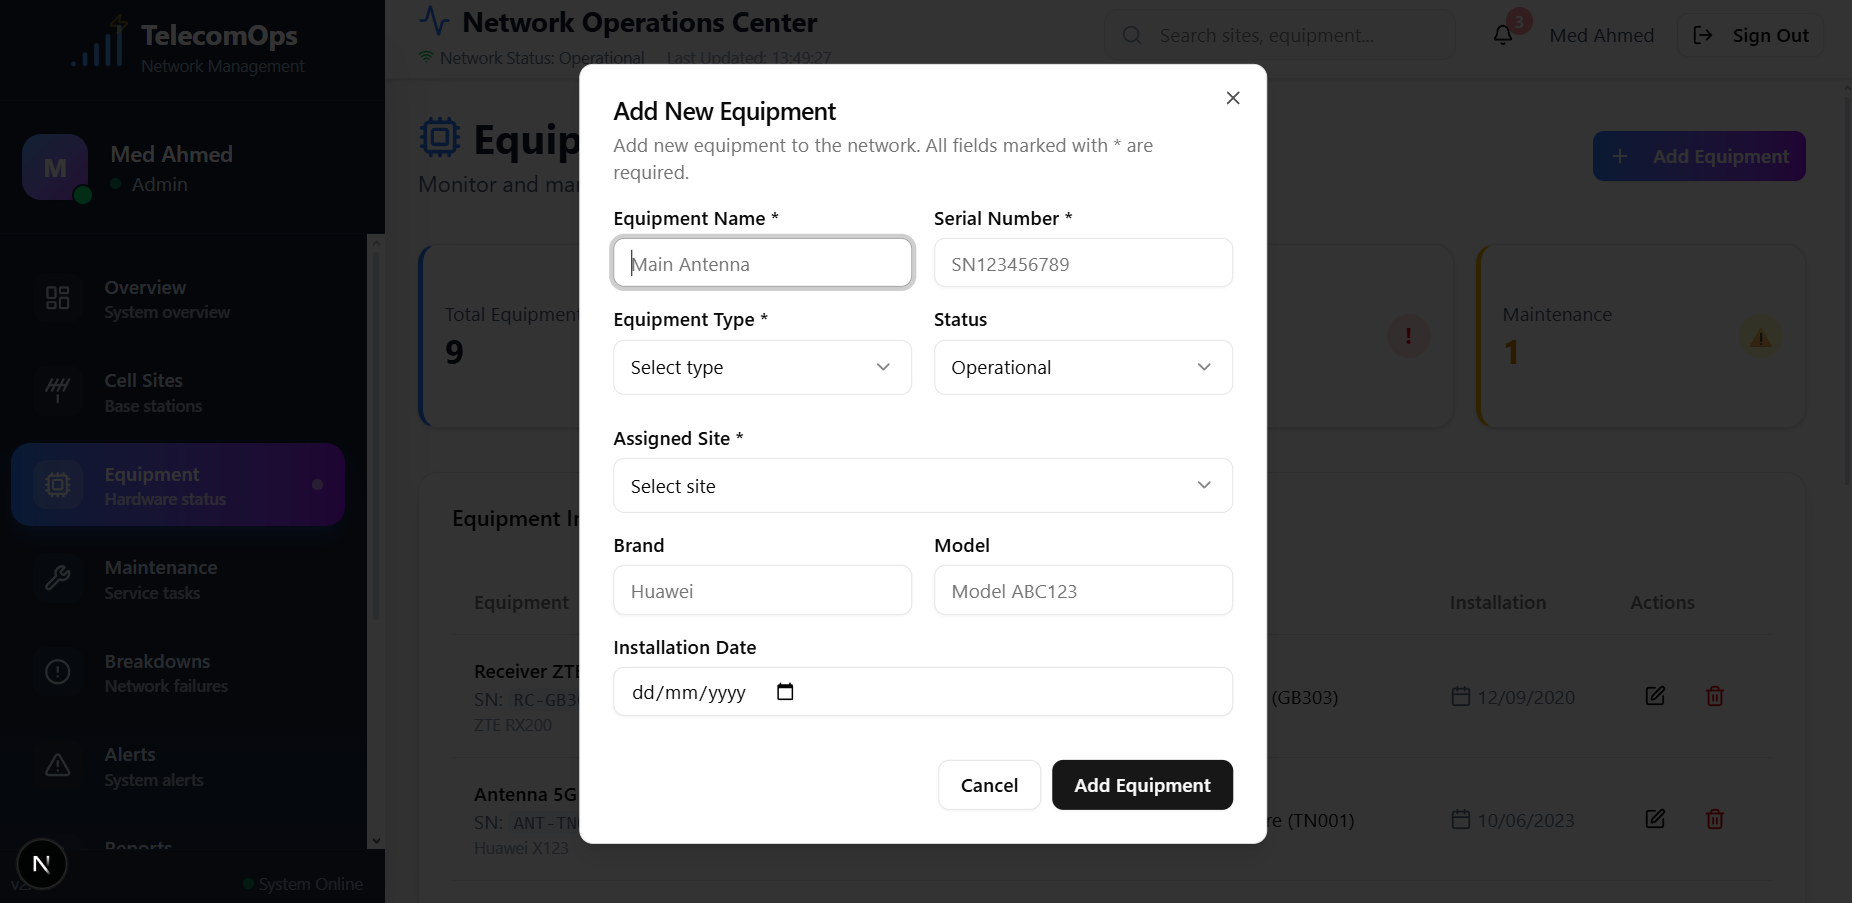
\includegraphics[width=0.6\linewidth]{img/chap_04/add_equipment_dialog.png}
    \caption{Add Equipment Modal}
    \label{fig:add_equipment_modal}
\end{figure}

The add equipment dialog implements required fields (name, serial, type, site) and optional fields (brand, model, installation date).

\begin{figure}[H]
    \centering
    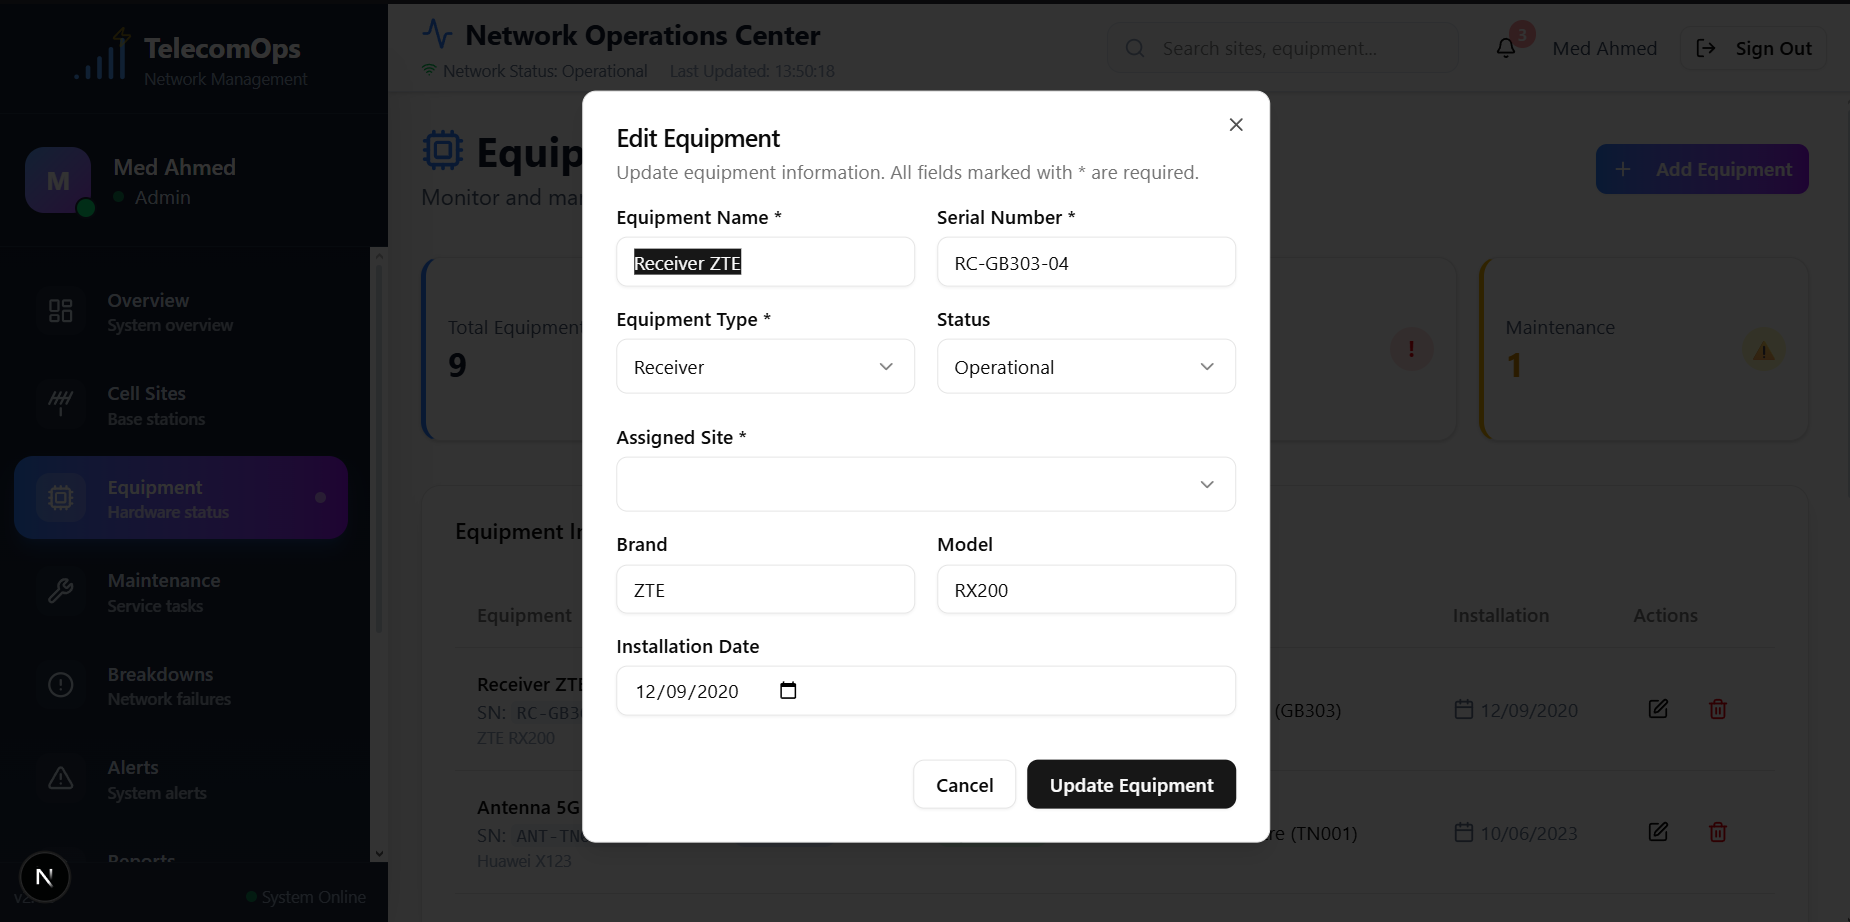
\includegraphics[width=0.6\linewidth]{img/chap_04/edit_equipment_dialog.png}
    \caption{Edit Equipment Modal}
    \label{fig:edit_equipment_modal}
\end{figure}

The edit dialog pre-populates with current information. Serial number remains immutable for traceability.

\section{Technical Challenges and Solutions}

\subsection{Serial Number Uniqueness Validation}

We implemented two-tier validation: client-side format validation for immediate feedback and server-side database queries with unique constraints for absolute enforcement. The equipment table's unique constraint provides database-level protection against duplicates.

\subsection{Equipment Status Management}

We implemented database CHECK constraints defining valid status values (operational, faulty, maintenance, offline) with automatic timestamp updates on \texttt{updated\_at} column, ensuring data integrity while maintaining complete state change history.

\subsection{Site-Equipment Relationship Integrity}

We implemented foreign key relationship with CASCADE deletion policy. The system displays warnings before site deletion showing affected equipment count. NOT NULL constraint on \texttt{site\_id} ensures every equipment maintains valid site association.

\section{Testing and Validation}

\subsection{Equipment CRUD Operations Testing}
Tests confirmed administrators perform all operations, engineers create and update but not delete, technicians view and update status only, and managers have read-only access with statistics.

\subsection{Serial Number Validation Testing}
Extensive testing ensured duplicate prevention. Concurrent creation attempts with identical serial numbers were successfully prevented by database constraints.

\subsection{Equipment Status Transition Testing}
Tests verified status changes update timestamps appropriately, invalid values are rejected, and modifications respect the role-based permission hierarchy.

\section{Conclusion}

This chapter described Sprint 2 focusing on equipment monitoring and inventory management. We performed comprehensive analysis using UML diagrams including class diagrams, use cases with inheritance hierarchy, and sequence diagrams. The implementation delivered complete equipment tracking with role-based access control and real-time status monitoring.

Sprint 2 extended Sprint 1 capabilities by introducing comprehensive equipment inventory management with serial number tracking, status monitoring, and warranty information. The hierarchical role-based permission system ensures logical permission escalation while maintaining security boundaries.

The equipment management system demonstrates effective integration of modern web technologies addressing telecommunications asset management requirements. Quality metrics exceeded targets with successful user acceptance testing across all four roles, establishing robust equipment tracking for network operations.
        \clearpage
        
        \chapter{Sprint 3: Breakdown Management and Intervention Planning}

\section{Introduction}

The third sprint focuses on developing the breakdown management and intervention planning modules, which are critical components for maintaining telecommunications network infrastructure. This sprint addresses both reactive and proactive aspects of network maintenance by implementing systems for reporting and tracking network failures while enabling preventive maintenance through scheduled interventions.

Network breakdowns represent urgent situations requiring immediate attention, such as power outages, equipment failures, or connectivity losses that can significantly impact service quality and affect thousands of users. The intervention planning module enables managers and engineers to schedule preventive maintenance tasks, assign technicians, and track activities. Together, these modules create a comprehensive maintenance management system balancing reactive problem-solving with proactive prevention strategies.

\section{Sprint Backlog}

Table \ref{tab:sprint3-backlog} presents the Sprint 3 backlog with eight main user stories covering breakdown management and intervention planning functionalities.

\begin{table}[H]
\centering
\scriptsize
\caption{Sprint 3 Backlog - Breakdown and Intervention Management}
\label{tab:sprint3-backlog}
\begin{tabular}{|p{2.8cm}|p{4cm}|p{5cm}|c|c|}
\hline
\textbf{Functionality} & \textbf{User Story} & \textbf{Tasks} & \textbf{Complexity} & \textbf{Hours} \\
\hline
Report Breakdown & As an engineer, I want to report network breakdowns for quick resolution & Create breakdown form, implement severity classification, auto-capture downtime start & High & 8h \\
\hline
Assign Breakdown & As a manager, I want to assign breakdowns to technicians & Implement assignment logic, send notifications, update status & Medium & 5h \\
\hline
Track Resolution & As a technician, I want to update breakdown status & Create status update interface, implement workflow transitions & Medium & 6h \\
\hline
Monitor Impact & As a manager, I want to see breakdown impact metrics & Display impacted users, calculate downtime, show statistics & Medium & 5h \\
\hline
Schedule Intervention & As an engineer, I want to schedule maintenance interventions & Create intervention form, check availability, prevent conflicts & High & 7h \\
\hline
Assign Technician & As a manager, I want to assign technicians to interventions & Implement assignment interface, check workload, send notifications & Medium & 5h \\
\hline
Update Status & As a technician, I want to update intervention progress & Create status interface, implement workflow, capture completion & Low & 4h \\
\hline
View History & As a manager, I want to view maintenance history & Create history view, filter by criteria, display statistics & Medium & 6h \\
\hline
\multicolumn{4}{|r|}{\textbf{Total:}} & \textbf{46h} \\
\hline
\end{tabular}
\end{table}

\section{Class Diagram}

Figure \ref{fig:sprint3-class} illustrates the class diagram introducing two core entities: \texttt{Breakdown} and \texttt{Intervention}, which work with existing entities for comprehensive maintenance management.

\begin{figure}[H]
\centering
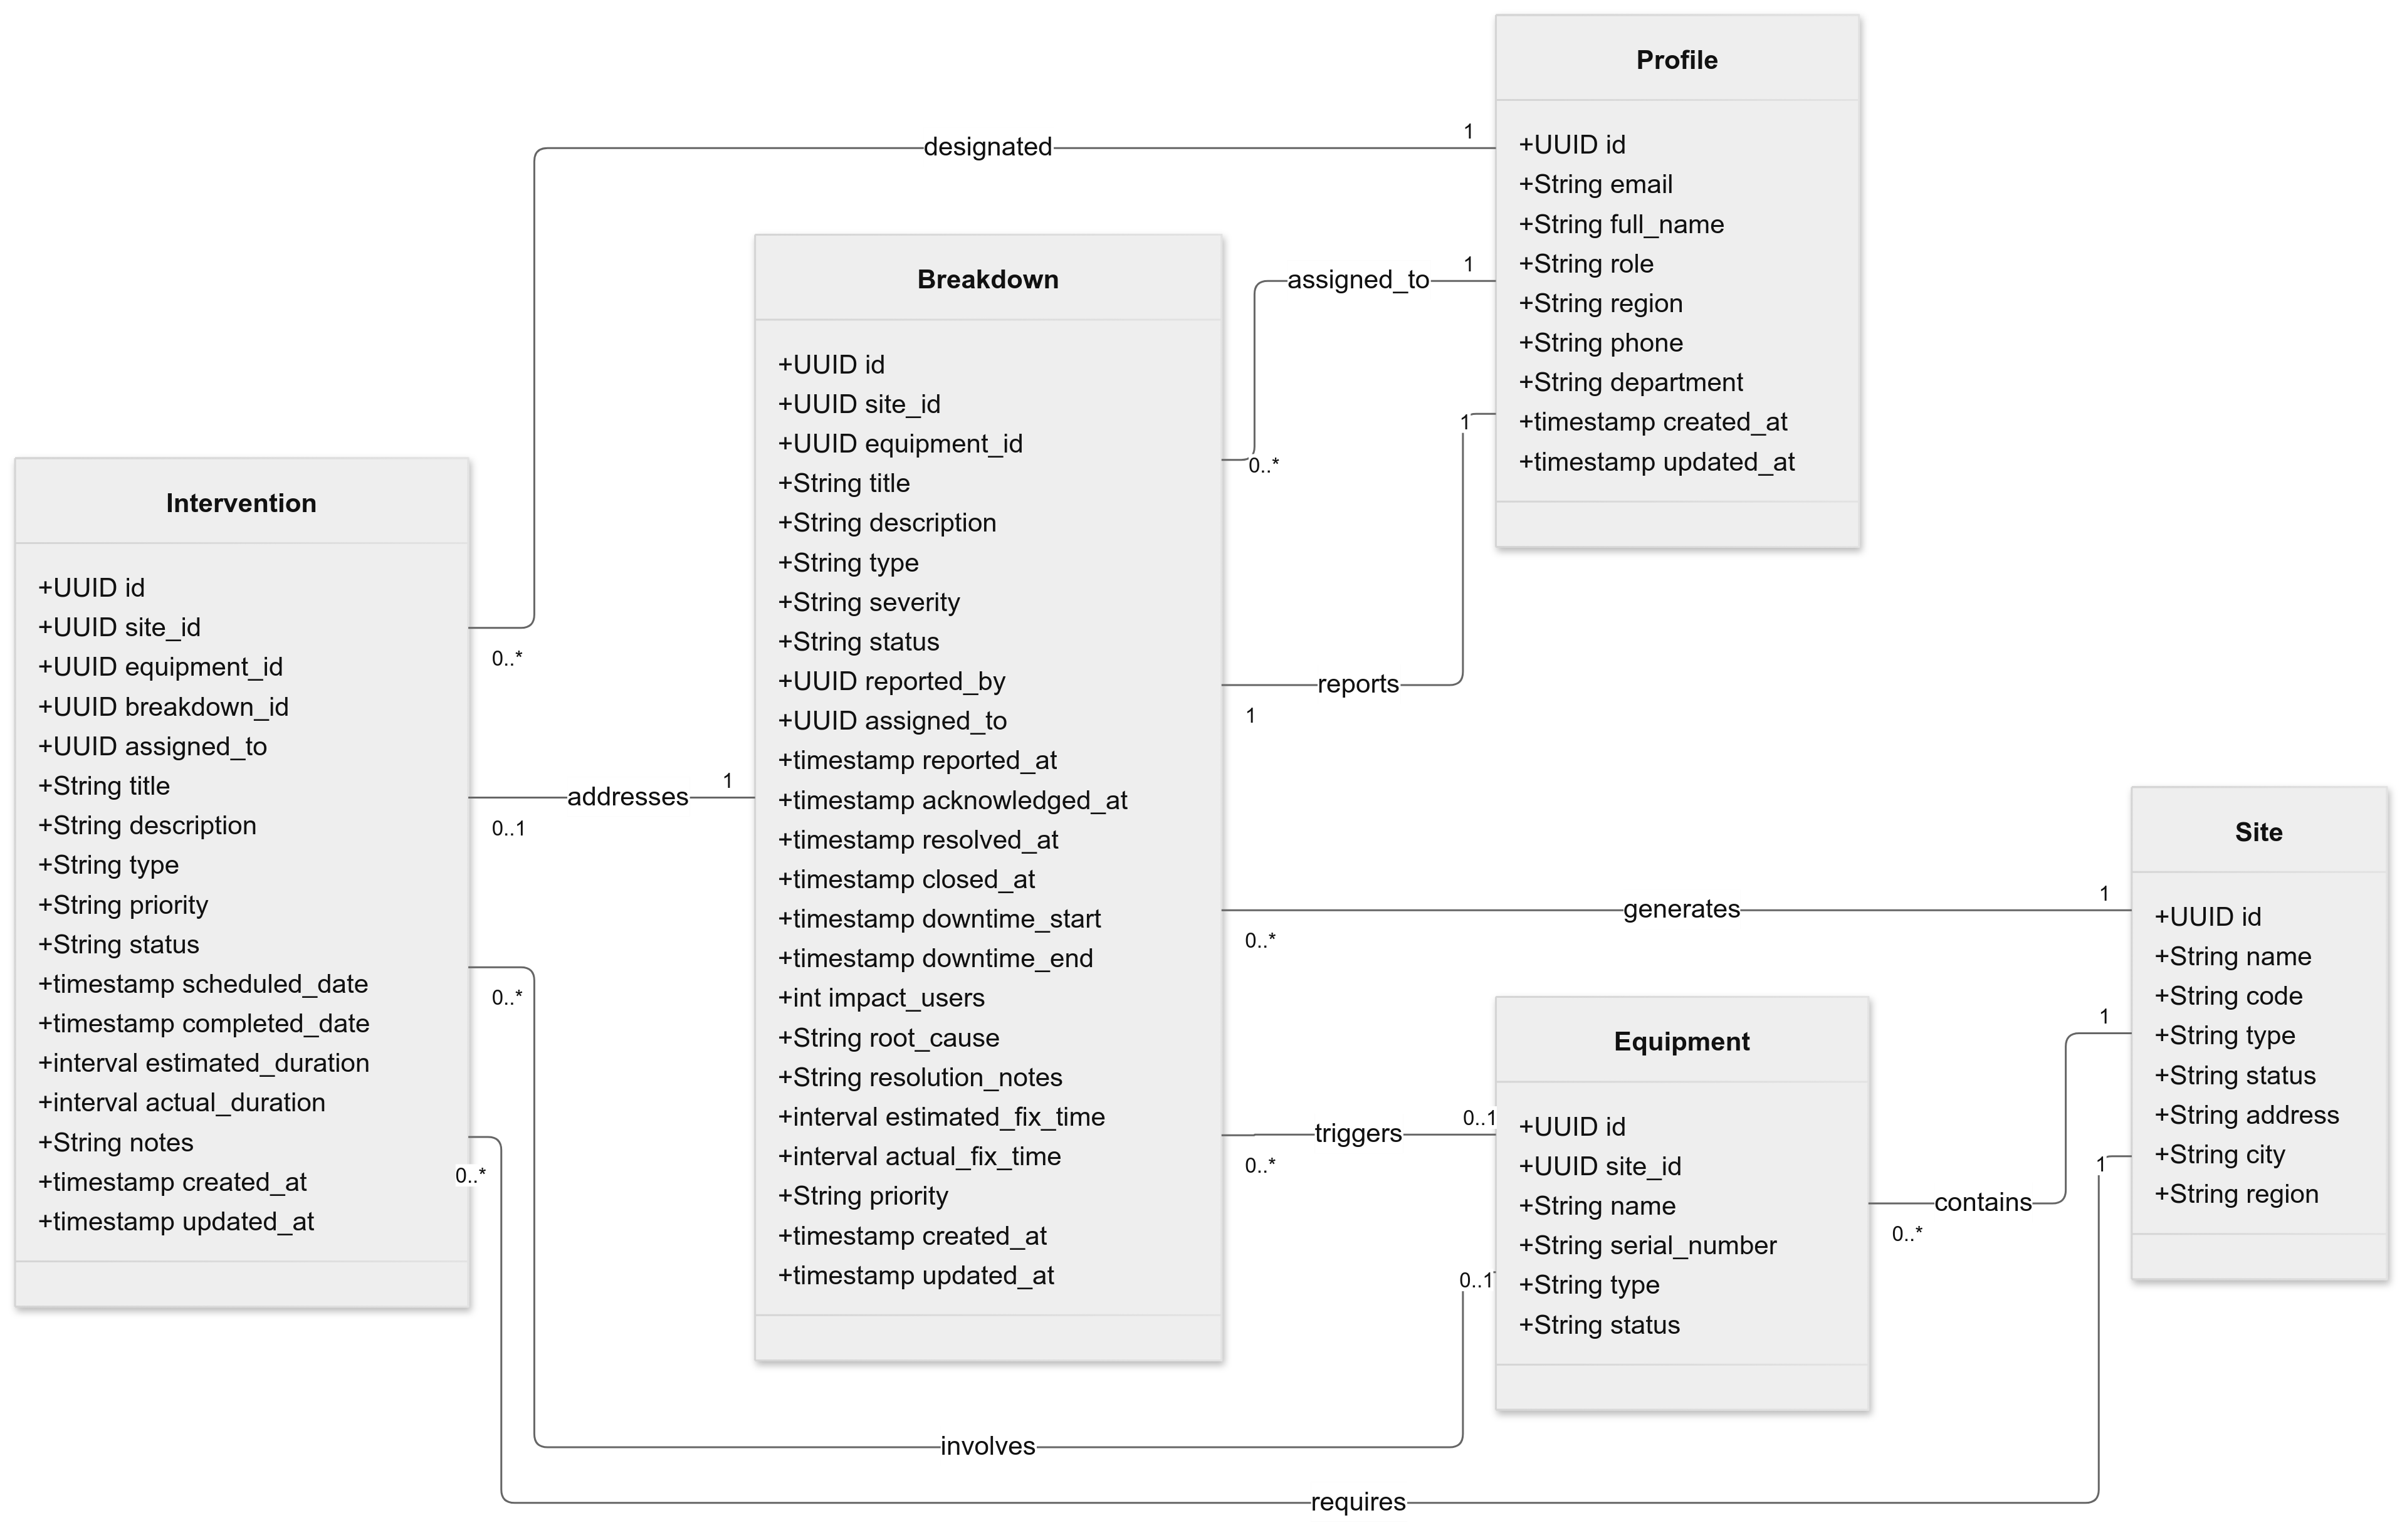
\includegraphics[width=0.7\textwidth]{img/chap_05/sprint3_class_diagram.png}
\caption{Class diagram for breakdown and intervention management}
\label{fig:sprint3-class}
\end{figure}

The \texttt{Breakdown} class represents network failures requiring immediate attention, tracking problem type, severity level (minor, major, critical), and status (open, investigating, in progress, resolved, closed). It maintains timestamps for the entire lifecycle and tracks user impact through \texttt{impact\_users} and downtime duration. The \texttt{Intervention} class manages scheduled maintenance activities, categorizing by type (preventive, corrective, installation, replacement) and priority. Both classes maintain relationships with \texttt{Profile}, \texttt{Site}, and \texttt{Equipment} entities, ensuring proper association with network infrastructure.

\section{Use Case Diagram}

Figure \ref{fig:sprint3-usecase} presents the use case diagram employing inheritance-based permission hierarchy where each role inherits all capabilities from roles below while adding specific functionalities.

\begin{figure}[H]
\centering
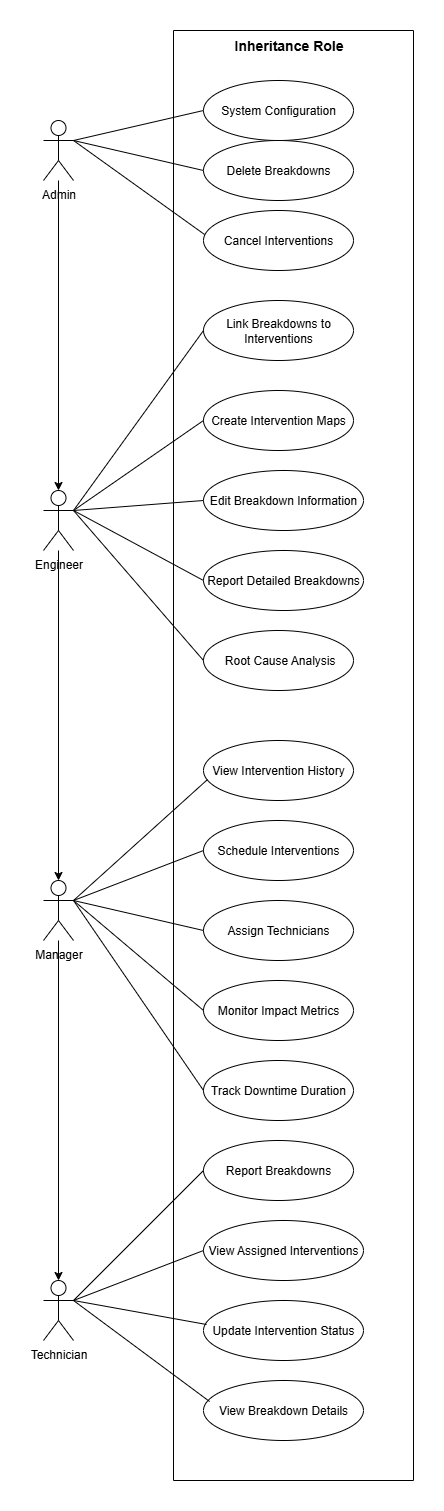
\includegraphics[width=0.7\textwidth]{img/chap_05/sprint3_usecase_diagram.png}
\caption{Use case diagram with role inheritance for Sprint 3}
\label{fig:sprint3-usecase}
\end{figure}

\textbf{Field Technicians} have base operational capabilities: view assigned interventions, update intervention status, report breakdowns, and view breakdown details. \textbf{Managers} inherit technician capabilities and add supervisory functions including viewing statistics, scheduling interventions, and assigning technicians. \textbf{Network Engineers} inherit manager capabilities and add technical analysis including root cause analysis and detailed planning. \textbf{Administrators} possess all privileges plus system management capabilities including deletion and configuration rights.

\section{Use Case Permissions Table}

Table \ref{tab:sprint3-permissions} details the permission matrix using Yes/No values indicating each role's capabilities within the inheritance hierarchy.

\begin{table}[H]
\centering
\scriptsize
\caption{Sprint 3 Use Case Permissions by Role}
\label{tab:sprint3-permissions}
\begin{tabular}{|p{5.5cm}|c|c|c|c|}
\hline
\textbf{Use Case} & \textbf{Technician} & \textbf{Manager} & \textbf{Engineer} & \textbf{Admin} \\
\hline
View Assigned Interventions & Yes & Yes & Yes & Yes \\
\hline
Update Intervention Status & Yes & Yes & Yes & Yes \\
\hline
Report Breakdowns & Yes & Yes & Yes & Yes \\
\hline
View Breakdown Details & Yes & Yes & Yes & Yes \\
\hline
View Intervention Statistics & No & Yes & Yes & Yes \\
\hline
View Breakdown Reports & No & Yes & Yes & Yes \\
\hline
Schedule Interventions & No & Yes & Yes & Yes \\
\hline
Assign Technicians & No & Yes & Yes & Yes \\
\hline
Track Downtime Duration & No & Yes & Yes & Yes \\
\hline
Monitor Impact Metrics & No & Yes & Yes & Yes \\
\hline
Root Cause Analysis & No & No & Yes & Yes \\
\hline
Create Intervention Plans & No & No & Yes & Yes \\
\hline
Edit Breakdown Information & No & No & Yes & Yes \\
\hline
Link Breakdowns to Equipment & No & No & Yes & Yes \\
\hline
Delete Breakdowns & No & No & No & Yes \\
\hline
Delete Interventions & No & No & No & Yes \\
\hline
Cancel Interventions & No & No & No & Yes \\
\hline
System Configuration & No & No & No & Yes \\
\hline
\end{tabular}
\end{table}

\section{Use Case Description}

Table \ref{tab:sprint3-usecase-detail} provides detailed description of the "Report Breakdown" use case.

\begin{table}[H]
\centering
\scriptsize
\caption{Detailed Description - Report Breakdown Use Case}
\label{tab:sprint3-usecase-detail}
\begin{tabular}{|p{3cm}|p{10.5cm}|}
\hline
\textbf{Element} & \textbf{Description} \\
\hline
\textbf{Use Case Name} & Report Breakdown \\
\hline
\textbf{Actor} & Network Engineer, Manager, Field Technician \\
\hline
\textbf{Description} & Allows users to report network breakdowns and failures requiring immediate attention with all necessary details for quick resolution \\
\hline
\textbf{Preconditions} & User authenticated with engineer/manager/technician role; Active sites exist; Breakdown types configured \\
\hline
\textbf{Postconditions} & Breakdown record created; Downtime tracking started; Notifications sent; Critical alerts escalated \\
\hline
\textbf{Main Flow} & 1. User clicks "Report Breakdown" button \newline 2. System displays breakdown form \newline 3. User enters title, description, type, and severity \newline 4. User selects affected site and equipment \newline 5. User estimates impacted users and fix time \newline 6. User submits form \newline 7. System validates required fields \newline 8. System creates breakdown with auto-captured timestamp \newline 9. System shows success confirmation \\
\hline
\textbf{Alternative Flow} & \textbf{A1 - Critical Severity:} At step 6, if severity is "Critical", system immediately notifies managers and highlights breakdown with urgent flag \newline \textbf{A2 - Equipment Selection:} At step 4, system loads equipment for selected site \\
\hline
\textbf{Exception Flow} & \textbf{E1 - Missing Fields:} At validation, if required fields empty, show error and return to form \newline \textbf{E2 - Invalid Data:} If negative values entered, show validation error \\
\hline
\end{tabular}
\end{table}

\section{Sequence Diagrams}

\subsection{Schedule Intervention Sequence}

Figure \ref{fig:sprint3-seq1} shows the interaction flow when scheduling a new maintenance intervention with conflict detection.

\begin{figure}[H]
\centering
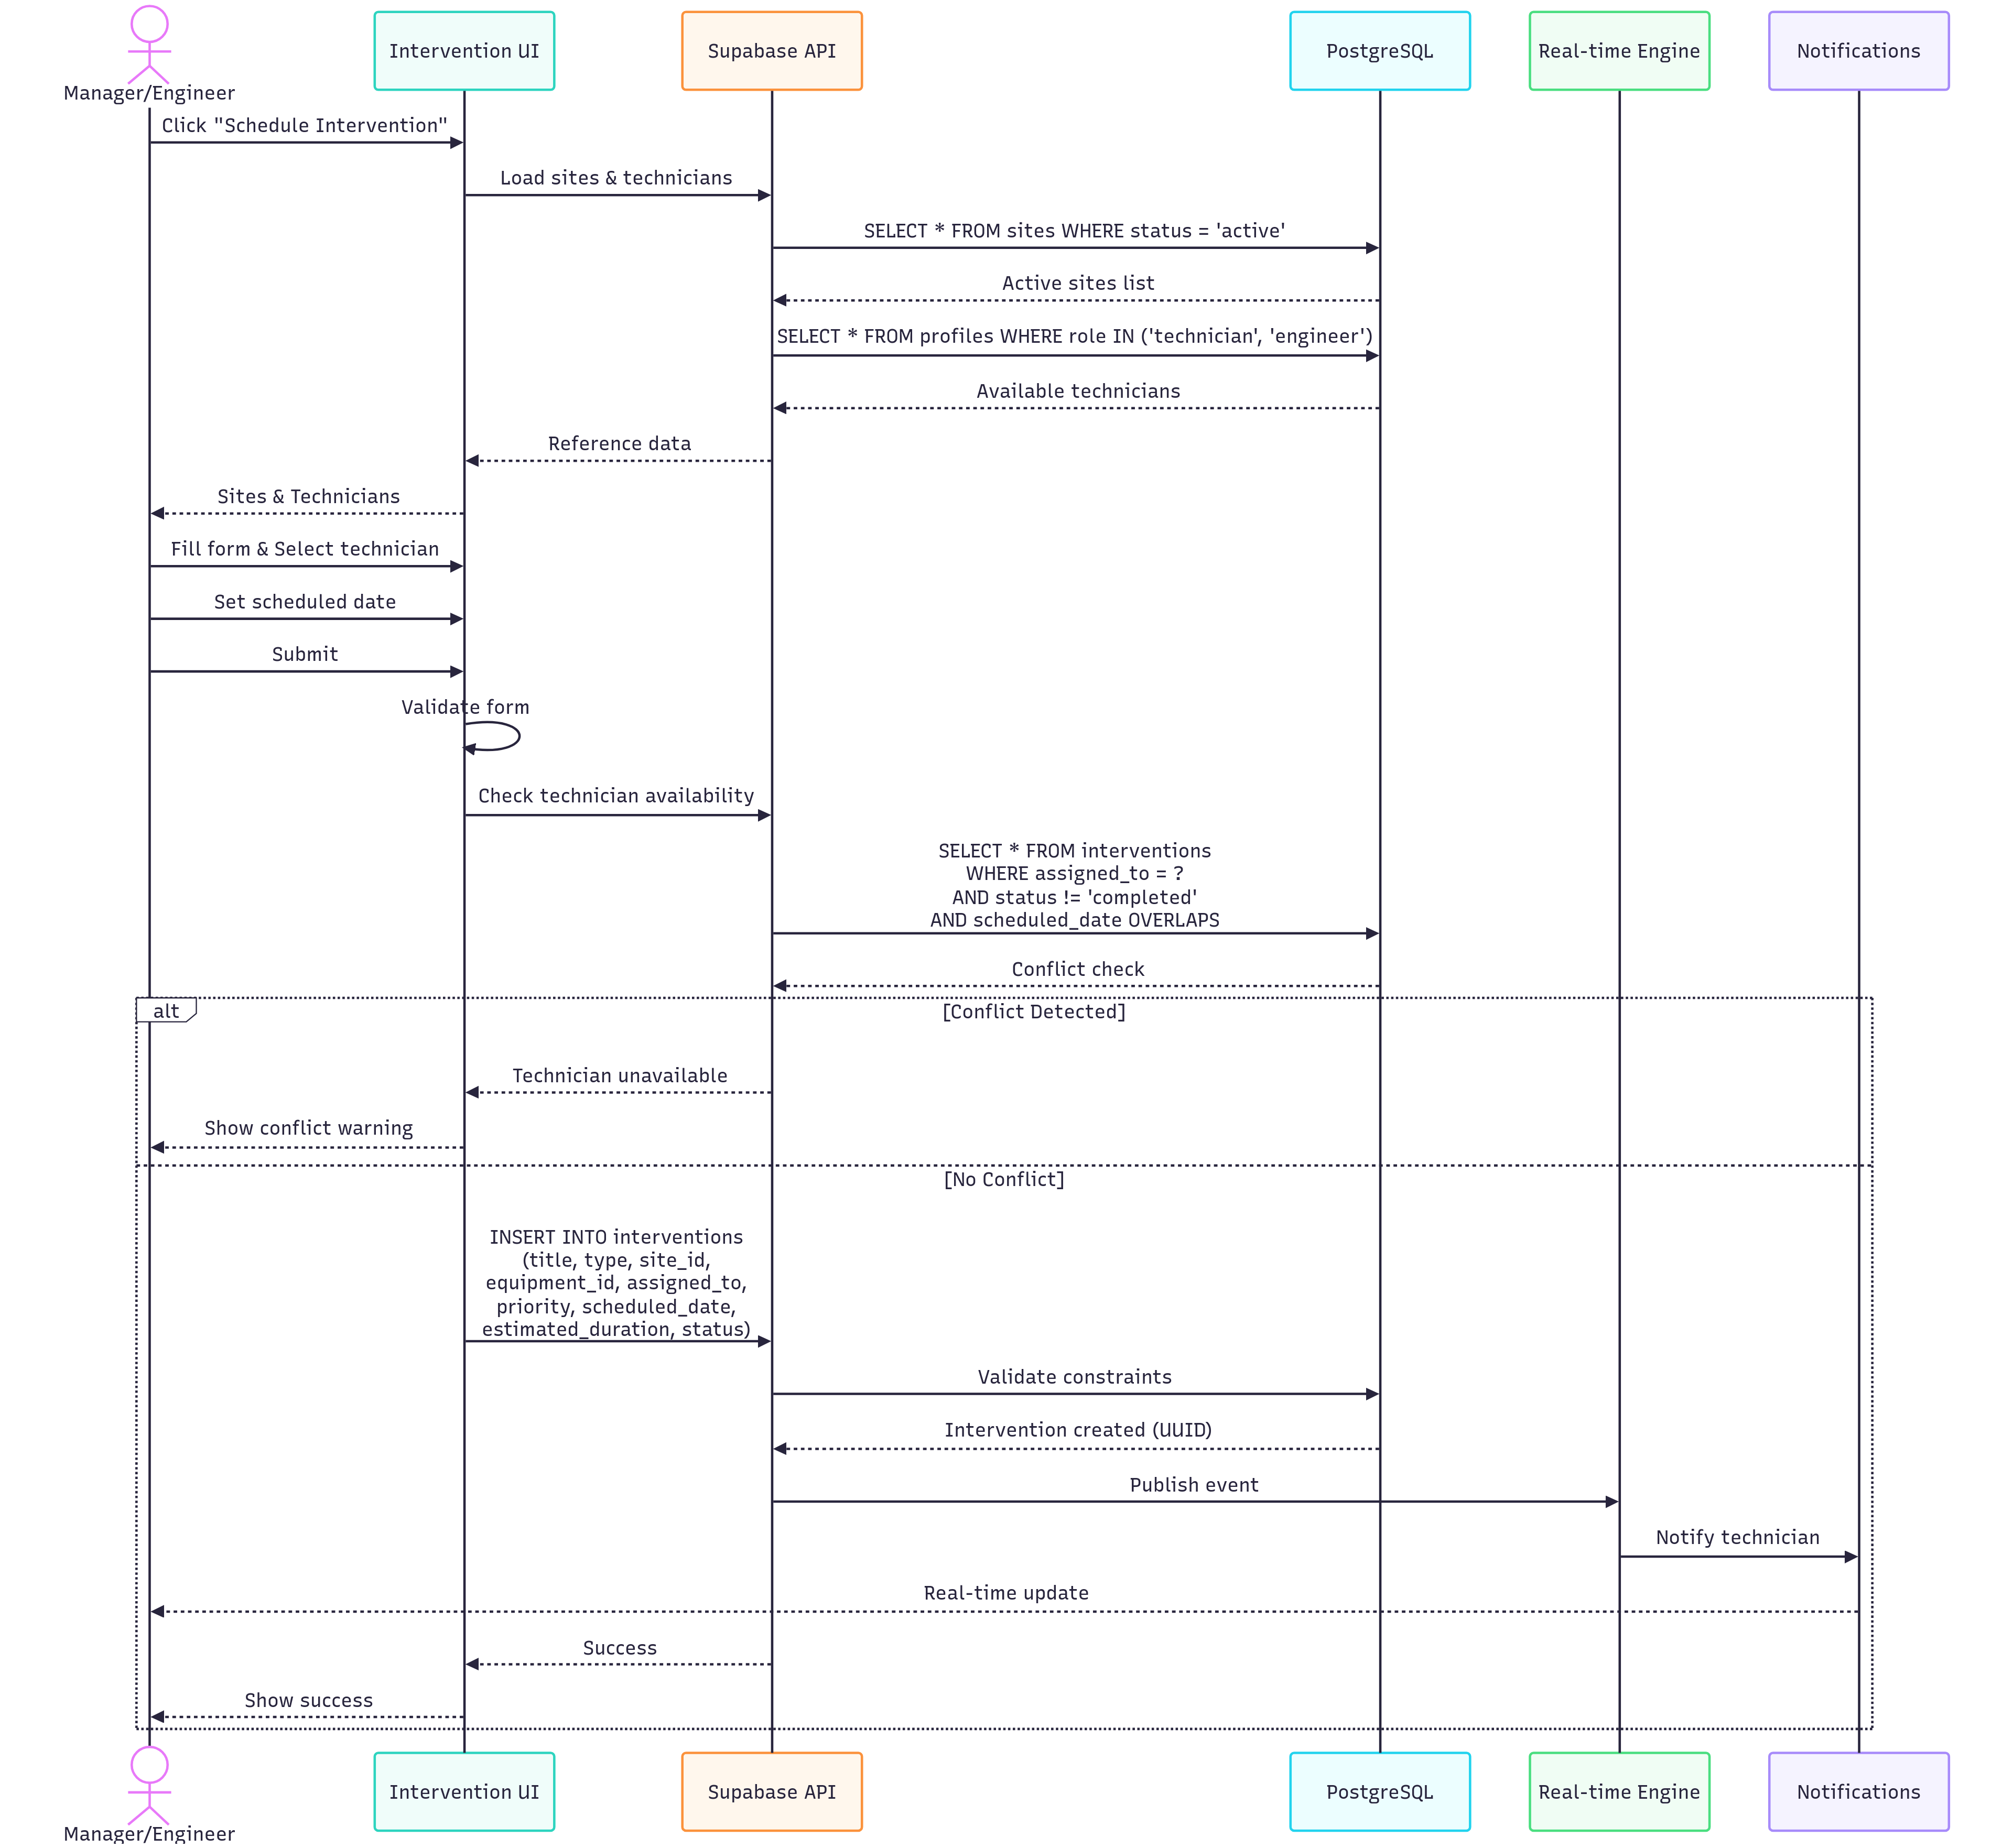
\includegraphics[width=0.7\textwidth]{img/chap_05/sprint3_sequence_intervention.png}
\caption{Sequence diagram for scheduling an intervention}
\label{fig:sprint3-seq1}
\end{figure}

\subsection{Report Breakdown Sequence}

Figure \ref{fig:sprint3-seq2} illustrates the workflow for reporting a network breakdown including critical severity escalation.

\begin{figure}[H]
\centering
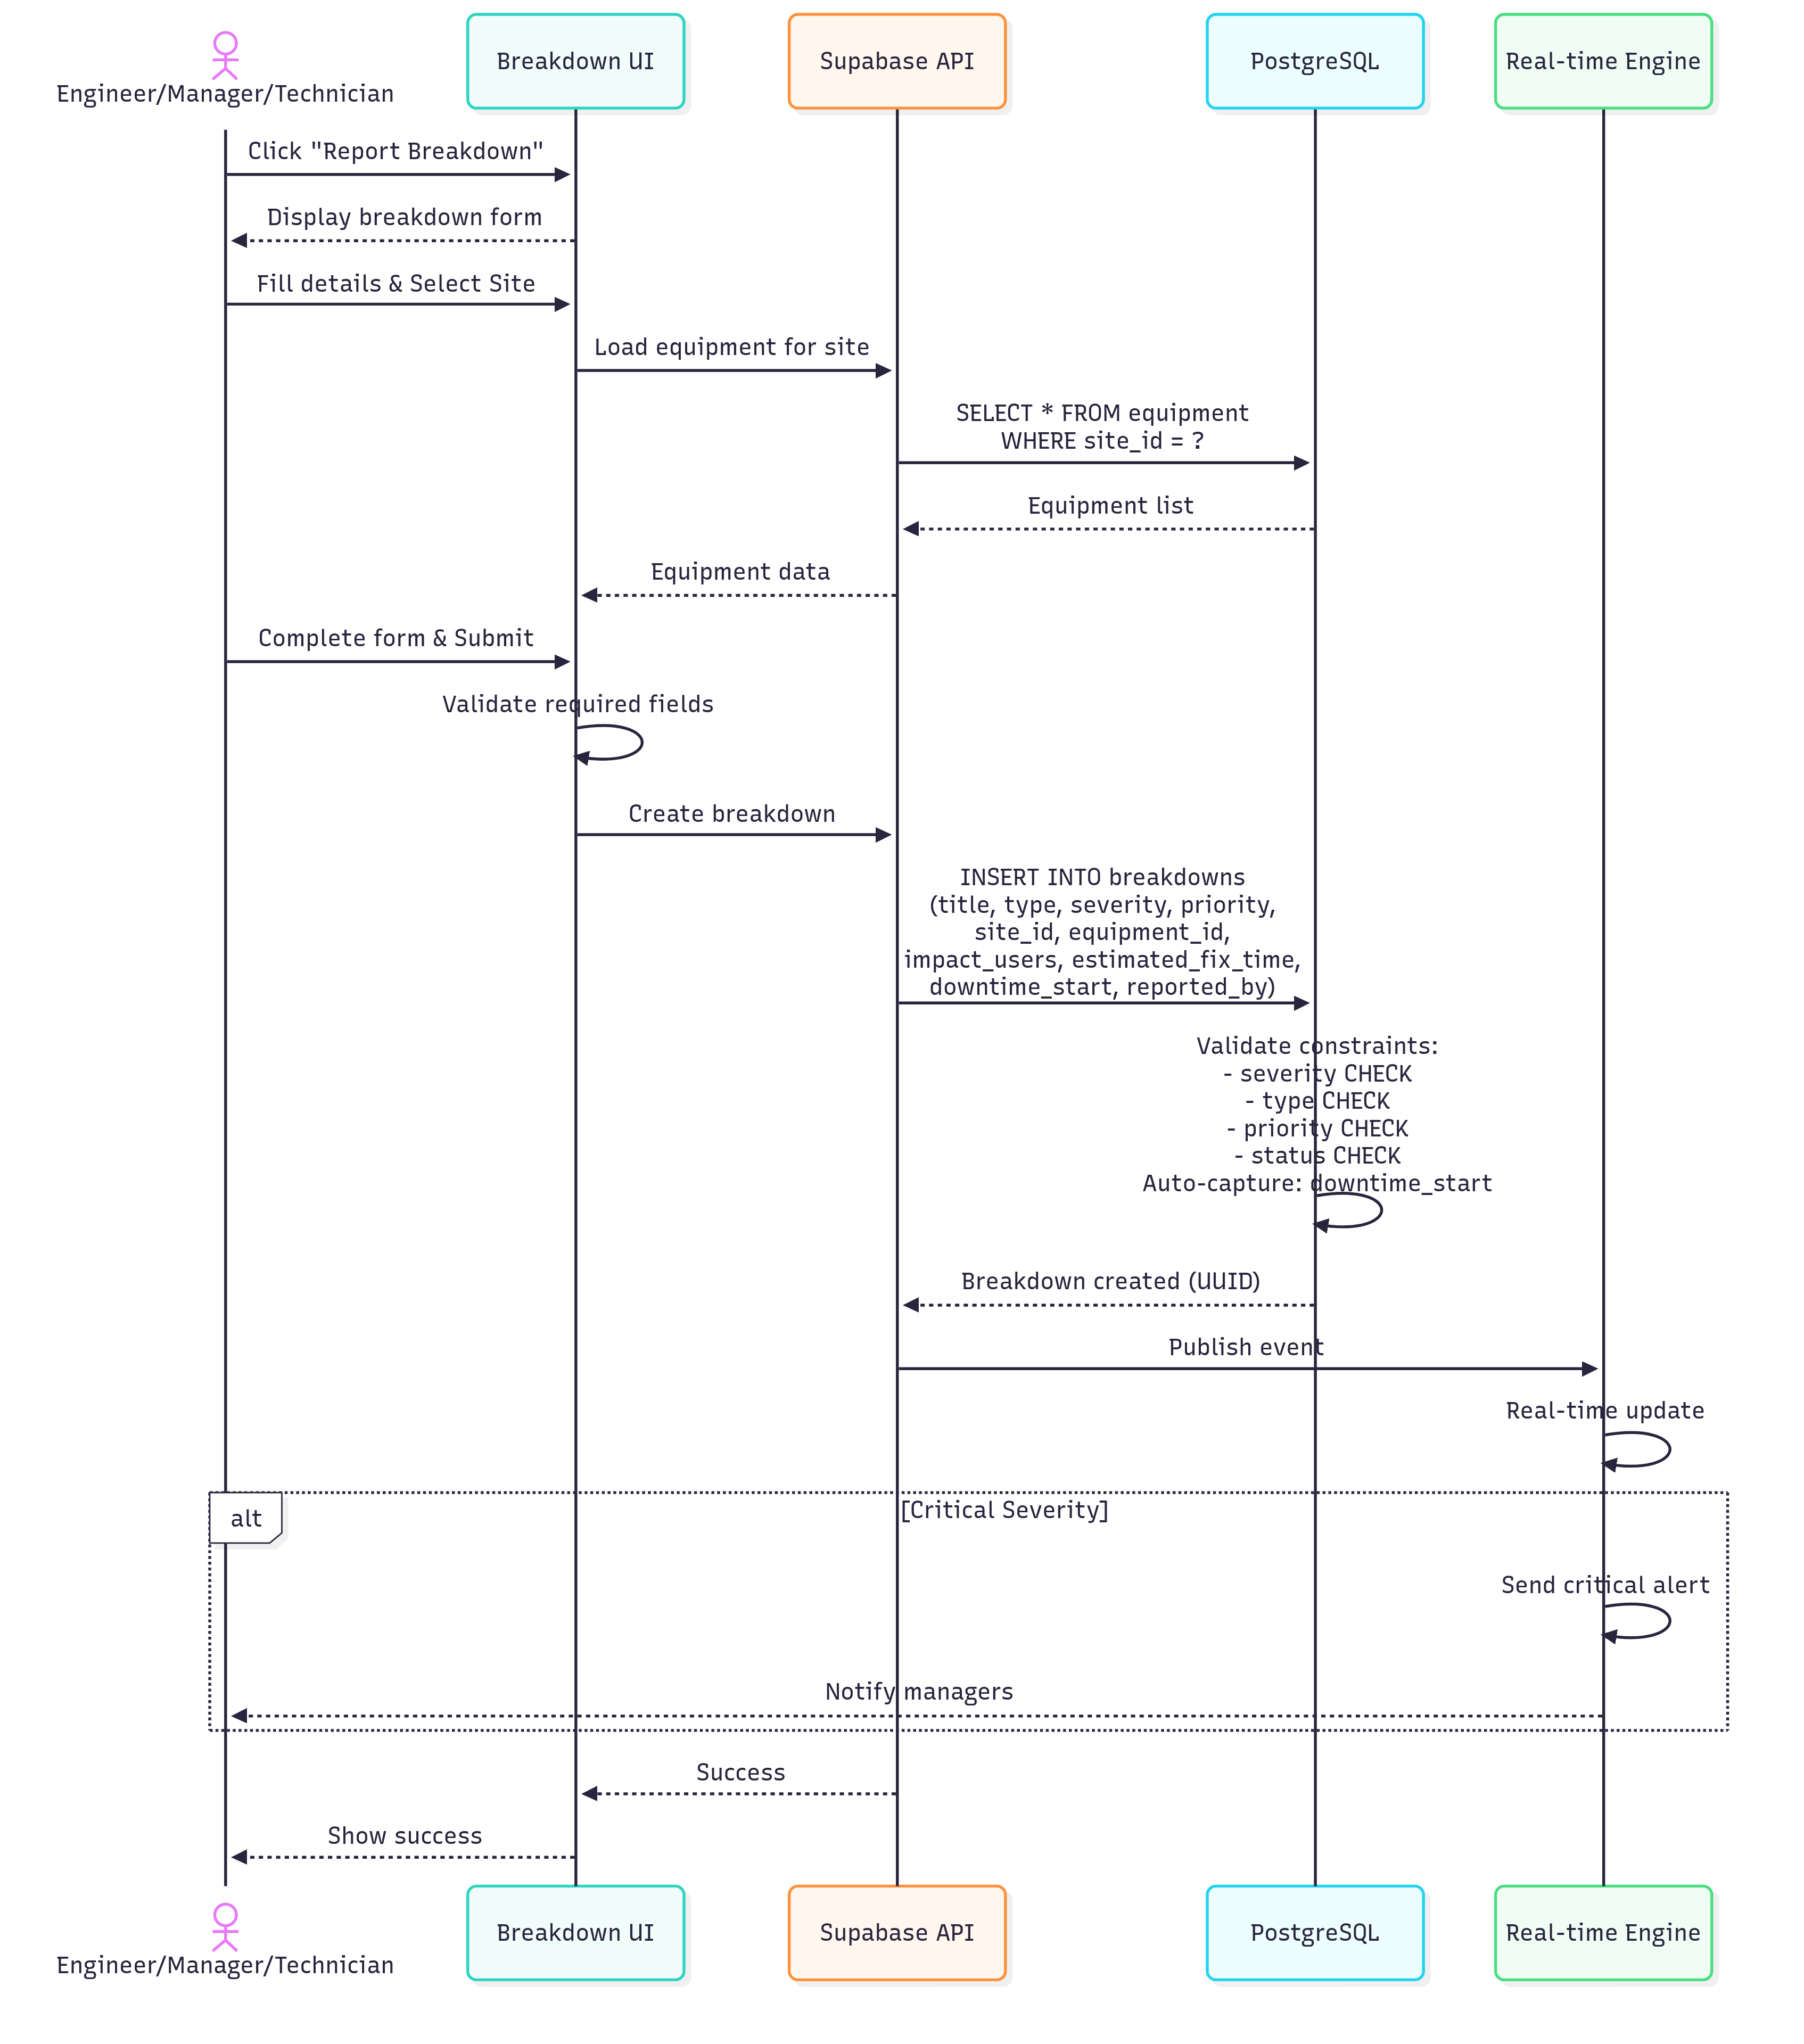
\includegraphics[width=0.7\textwidth]{img/chap_05/sprint3_sequence_breakdown.png}
\caption{Sequence diagram for reporting a breakdown}
\label{fig:sprint3-seq2}
\end{figure}

\section{Implementation}

This section presents the implemented interfaces for breakdown management and intervention planning modules.

\subsection{Intervention Management Dashboard}

Figure \ref{fig:sprint3-impl1} shows the intervention management interface with quick statistics and task listing.

\begin{figure}[H]
\centering
\fbox{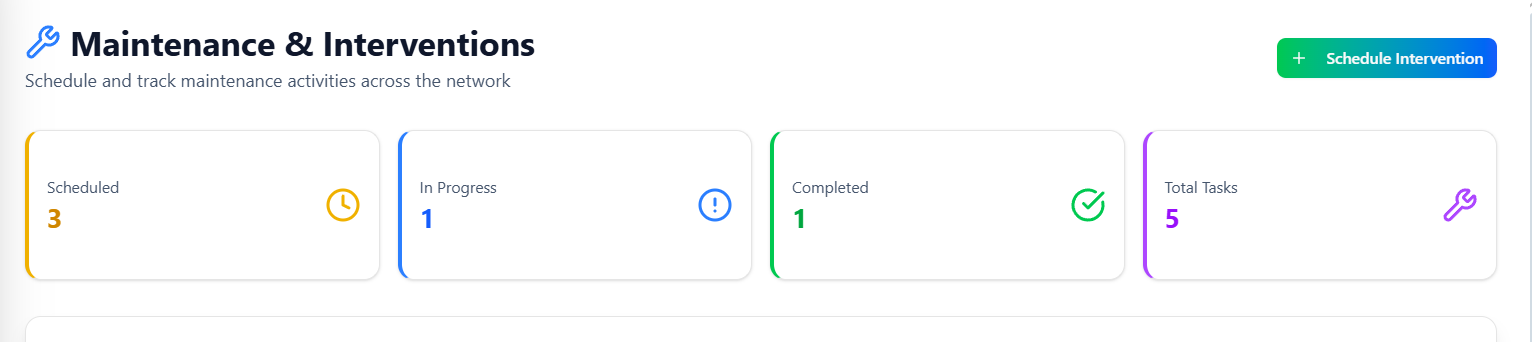
\includegraphics[width=0.70\textwidth]{img/chap_05/screenshot_interventions_dashboard.png}}
\caption{Intervention management dashboard with statistics and task list}
\label{fig:sprint3-impl1}
\end{figure}

The dashboard displays quick statistics showing scheduled, in-progress, and completed interventions. The interventions table presents each task with type, priority, status, site, assigned technician, and scheduled date using color-coded badges for quick identification.

\subsection{Breakdown Management Dashboard}

Figure \ref{fig:sprint3-impl2} displays the breakdown management interface tracking network failures.

\begin{figure}[H]
\centering
\fbox{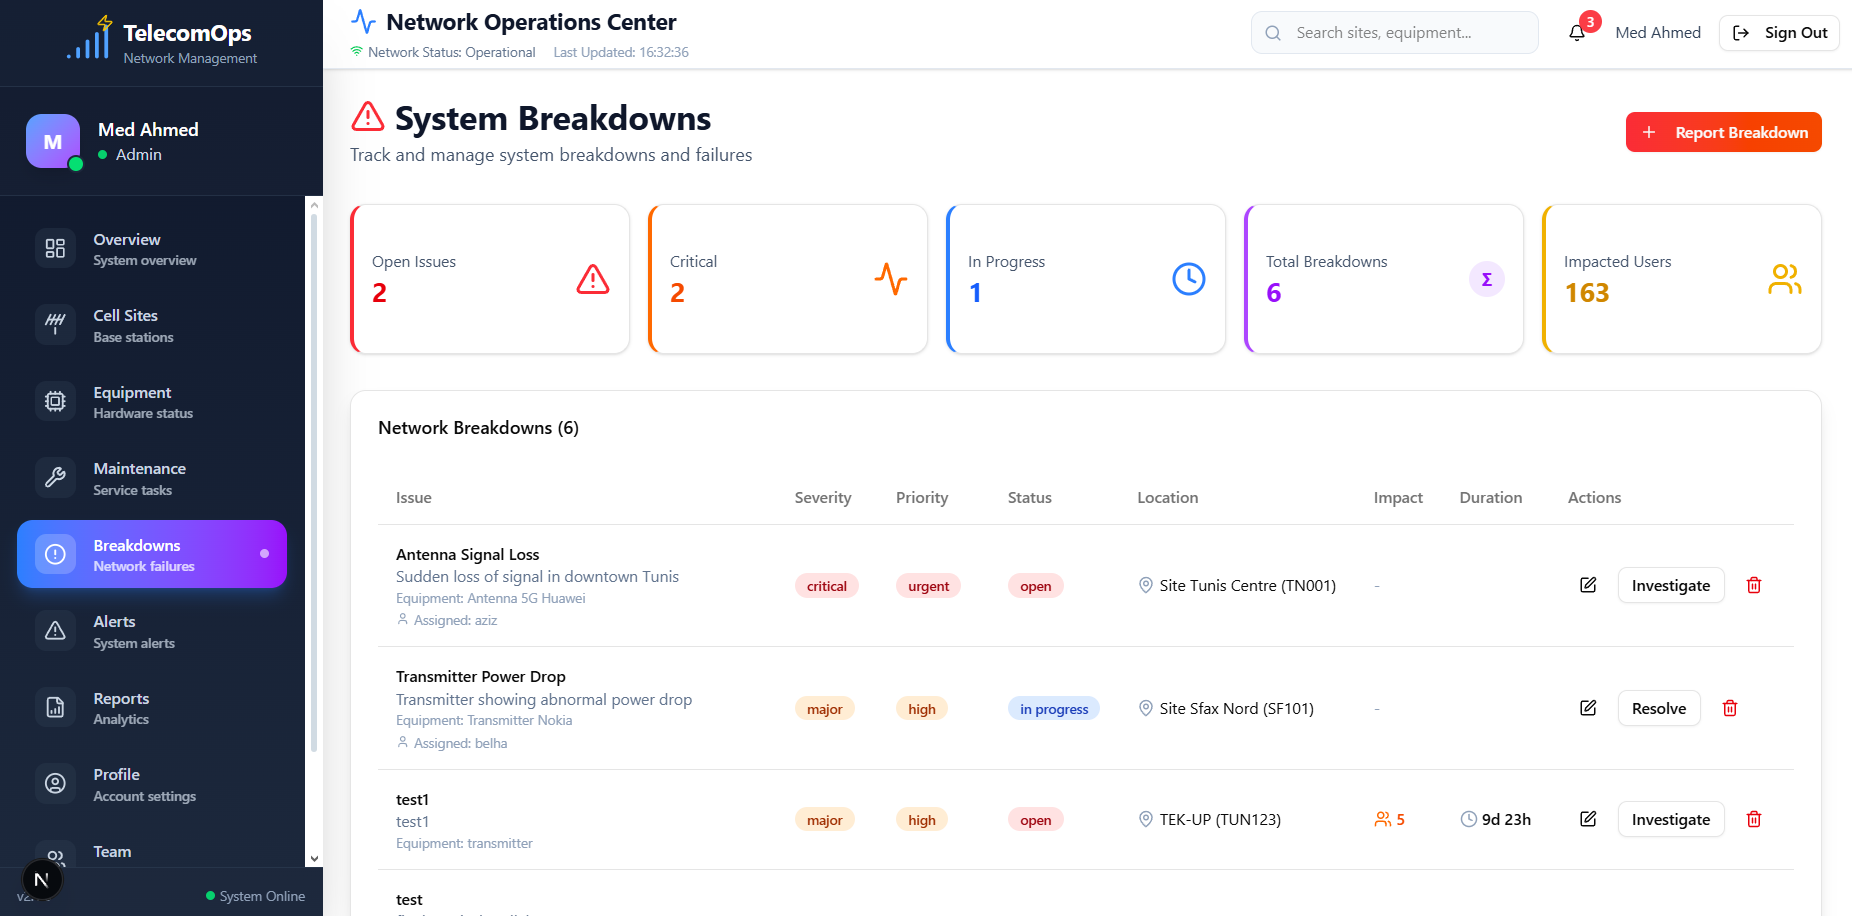
\includegraphics[width=0.70\textwidth]{img/chap_05/screenshot_breakdowns_dashboard.png}}
\caption{Breakdown management dashboard showing active issues and statistics}
\label{fig:sprint3-impl2}
\end{figure}

The dashboard features metrics for open issues, critical breakdowns, in-progress resolutions, total breakdowns, and impacted users. The table displays severity, priority, status, location, impact, and duration with action buttons for workflow progression.

\subsection{Schedule Intervention Form}

Figure \ref{fig:sprint3-impl3} presents the intervention scheduling form interface.

\begin{figure}[H]
\centering
\fbox{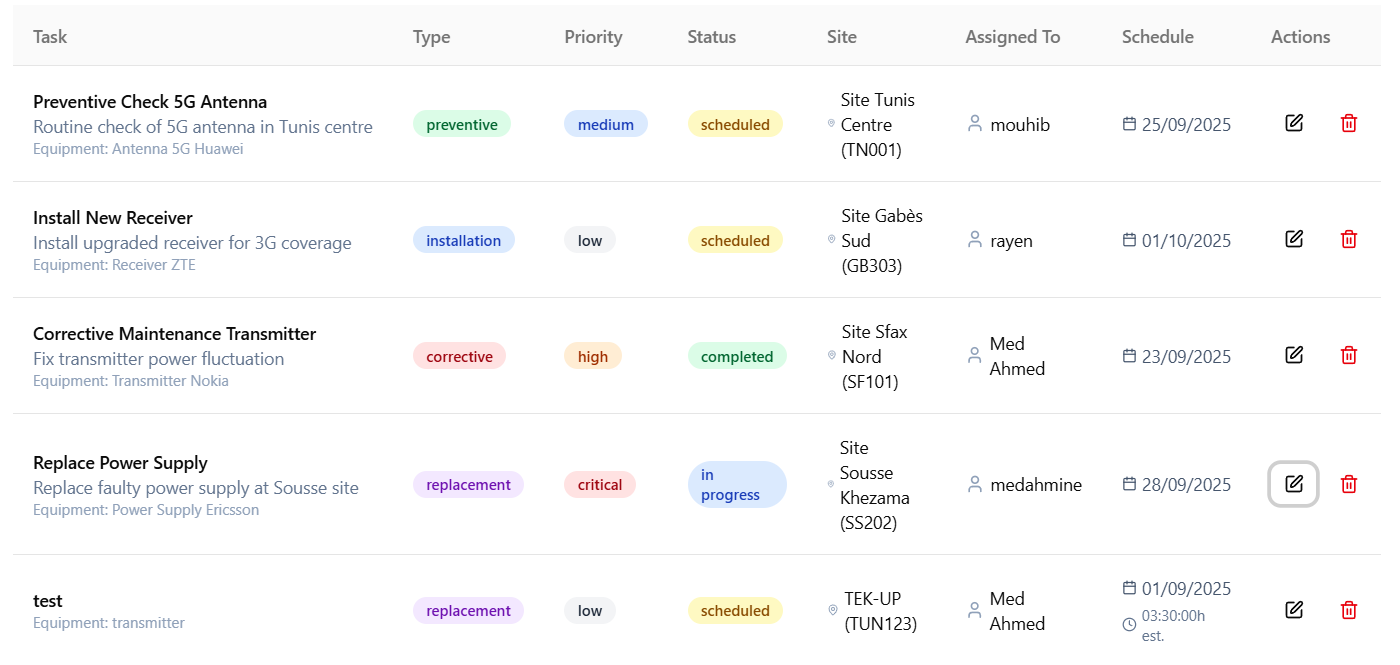
\includegraphics[width=0.7\textwidth]{img/chap_05/screenshot_schedule_intervention.png}}
\caption{Schedule intervention form with validation and conflict detection}
\label{fig:sprint3-impl3}
\end{figure}

The form includes fields for task title, intervention type, priority, target site, equipment selection, technician assignment, scheduled date, and estimated duration with comprehensive validation and conflict detection.

\subsection{Report Breakdown Form}

Figure \ref{fig:sprint3-impl4} shows the breakdown reporting form for incident documentation.

\begin{figure}[H]
\centering
\fbox{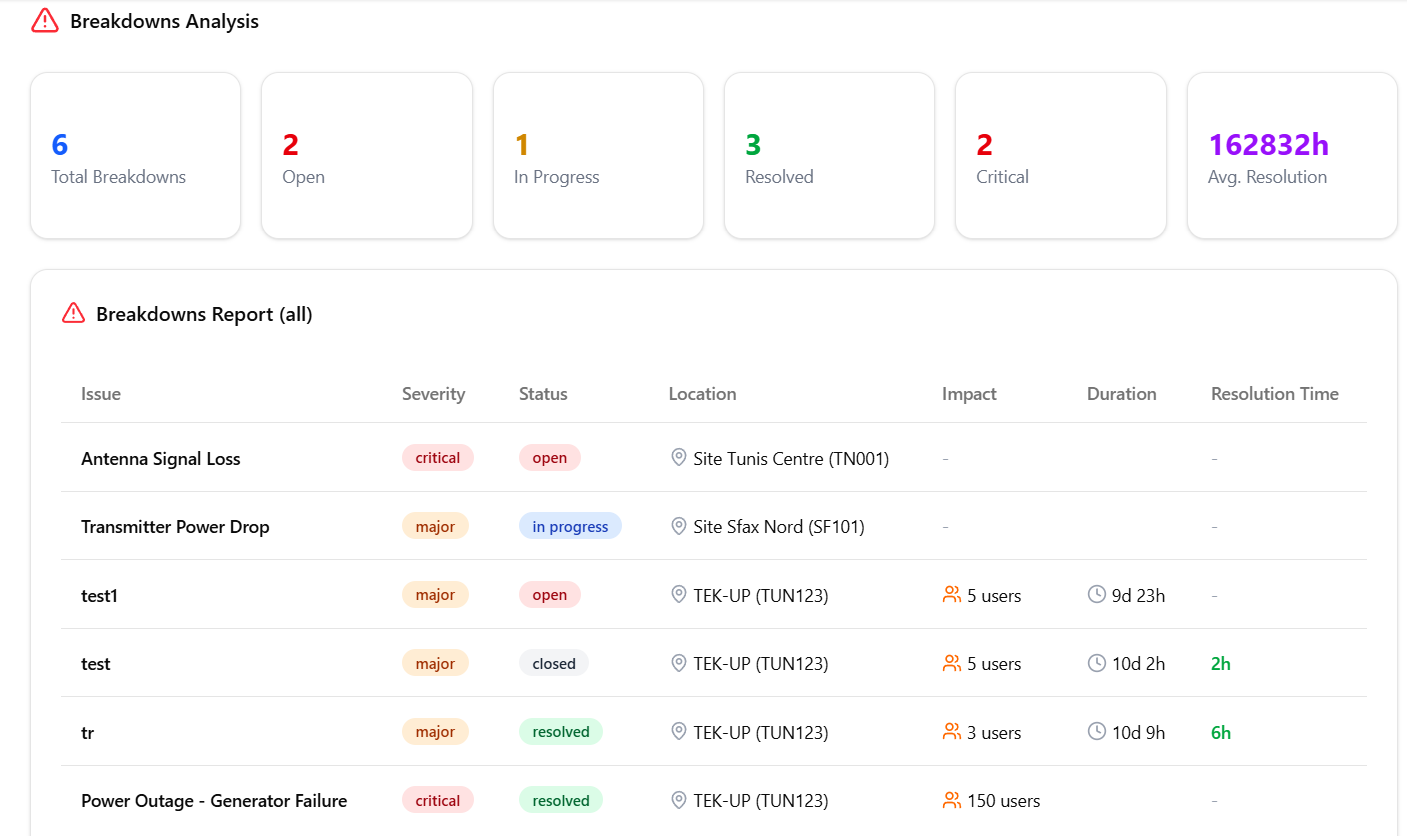
\includegraphics[width=0.7\textwidth]{img/chap_05/screenshot_report_breakdown.png}}
\caption{Report breakdown form with severity classification and impact estimation}
\label{fig:sprint3-impl4}
\end{figure}

The form enables quick incident reporting with breakdown type, severity classification, affected site and equipment selection, impact estimation, and automatic downtime tracking with critical severity escalation.

\section{Technical Challenges and Solutions}

\subsection{Technician Assignment Conflict Detection}

\textbf{Challenge:} Preventing double-booking when scheduling interventions required detecting time overlaps with variable-duration tasks stored as timestamps.

\textbf{Solution:} Implemented conflict detection algorithm querying existing interventions for assigned technician and checking time overlaps. The system calculates intervention end time by adding estimated duration to scheduled date, compares against proposed time slot, and displays warnings for conflicts while allowing managers flexibility in resource allocation.

\subsection{Real-time Downtime Duration Calculation}

\textbf{Challenge:} Displaying continuously updating breakdown duration in human-readable format without constant database queries or page refreshes.

\textbf{Solution:} Implemented client-side calculation function computing elapsed time from stored downtime start timestamp. The function intelligently formats durations: under 1 hour as "< 1h", under 24 hours as hours, and longer as days plus hours. The UI component recalculates periodically, providing accurate current information without database load.

\subsection{Cascading Status Updates and Timestamp Management}

\textbf{Challenge:} Multiple status transitions requiring automatic timestamp capture (acknowledged, resolved, closed) without manual entry while triggering related actions like downtime calculation.

\textbf{Solution:} Implemented automatic timestamp capture in update logic by detecting status changes and adding appropriate timestamp fields. When breakdown status becomes "investigating", system sets acknowledged timestamp; when "resolved", sets both resolved and downtime end timestamps enabling automatic duration calculation. This ensures data consistency and provides accurate audit trails.

\section{Testing and Validation}

\subsection{Functional Testing}

Functional testing verified all features work correctly. We tested breakdown reporting with various types and severities, confirming critical breakdowns trigger immediate manager notifications. Intervention scheduling validated different task types, technician assignment, and conflict detection. Status workflow transitions were tested through all states with automatic timestamp capture verification. CRUD operations for both breakdowns and interventions ensured data integrity.

\subsection{Integration Testing}

Integration testing ensured Sprint 3 components work with existing modules. We tested site and equipment integration by selecting resources when reporting breakdowns and scheduling interventions. Authentication and authorization were verified with different roles ensuring proper permission hierarchy. Real-time notifications confirmed managers receive critical breakdown alerts. Database relationships verified foreign key enforcement preventing orphaned records. Dashboard statistics validated accurate calculations.

\subsection{User Acceptance Testing}

Tunisia Telecom staff tested features in realistic scenarios. Technicians tested mobile-responsive interfaces for field reporting and confirmed easy form usage. Managers tested scheduling workflows, validating conflict detection and priority indicators. Engineers tested breakdown reporting with technical details, confirming adequate documentation fields and proper status transitions. Overall feedback was positive, with users appreciating clear visual indicators, intuitive workflows, and real-time updates.

\section{Conclusion}

Sprint 3 successfully delivered comprehensive breakdown management and intervention planning capabilities significantly enhancing TelecomOps maintenance functionality. The breakdown management system enables rapid incident reporting with detailed classification, automatic downtime tracking, and workflow-guided resolution. Critical severity escalation ensures urgent issues receive immediate attention, minimizing customer impact.

The intervention planning module enables preventive maintenance scheduling with technician assignment, progress tracking, and conflict detection preventing scheduling errors. Together, these modules create a complete maintenance solution balancing reactive and proactive approaches. Integration with existing modules ensures proper infrastructure association, while role-based permissions provide appropriate access levels. Real-time notifications keep stakeholders informed enabling rapid response.

Technical challenges around conflict detection and timestamp management were successfully resolved through careful validation logic and automatic data capture. Testing confirmed functional requirements and proper integration. Sprint 3 establishes foundation for advanced maintenance analytics and predictive capabilities, with comprehensive data enabling pattern analysis to optimize maintenance schedules and improve network reliability.
        \clearpage
        
        \chapter{Sprint 4: Alerts Management and Energy Consumption Monitoring}

\section{Introduction}

Sprint 4 represents a critical advancement in the TelecomOps platform, focusing on two essential subsystems: the Alerts Management System and the Energy Consumption Monitoring System. These implementations address critical operational requirements for proactive network management and energy efficiency optimization.

The Alerts Management System provides real-time notification capabilities for network anomalies, equipment failures, and maintenance requirements with status transitions from active to acknowledged to resolved. The Energy Consumption Monitoring System enables comprehensive tracking and analysis of power consumption across network sites with automatic cost calculation, visual analytics, and threshold-based alerting.

Both systems integrate seamlessly with existing platform architecture, leveraging Supabase real-time subscriptions, PostgreSQL with Row-Level Security, and Next.js 14 capabilities. This sprint delivers eight user stories encompassing automated alert generation, real-time notifications, energy recording, trend visualization, and consumption analytics.

\section{Sprint Backlog}

\begin{table}[htbp]
\centering
\caption{Sprint 4 Backlog - User Stories}
\small
\begin{tabular}{|p{0.8cm}|p{9cm}|p{1.8cm}|}
\hline
\textbf{ID} & \textbf{User Story} & \textbf{Priority} \\
\hline
US-4.1 & As a system, I want to automatically create alerts when equipment faults are detected & Critical \\
\hline
US-4.2 & As a manager, I want to acknowledge critical alerts to track response time & High \\
\hline
US-4.3 & As an engineer, I want to resolve alerts after fixing issues & High \\
\hline
US-4.4 & As a user, I want real-time notifications for critical alerts & Critical \\
\hline
US-4.5 & As a manager, I want to record energy consumption data for each site & High \\
\hline
US-4.6 & As an engineer, I want to view energy consumption trends with charts & Medium \\
\hline
US-4.7 & As a manager, I want to calculate energy costs automatically & High \\
\hline
US-4.8 & As an admin, I want to track consumption per day and identify patterns & Medium \\
\hline
\end{tabular}
\end{table}

\section{Class Diagram}

\begin{figure}[H]
\centering
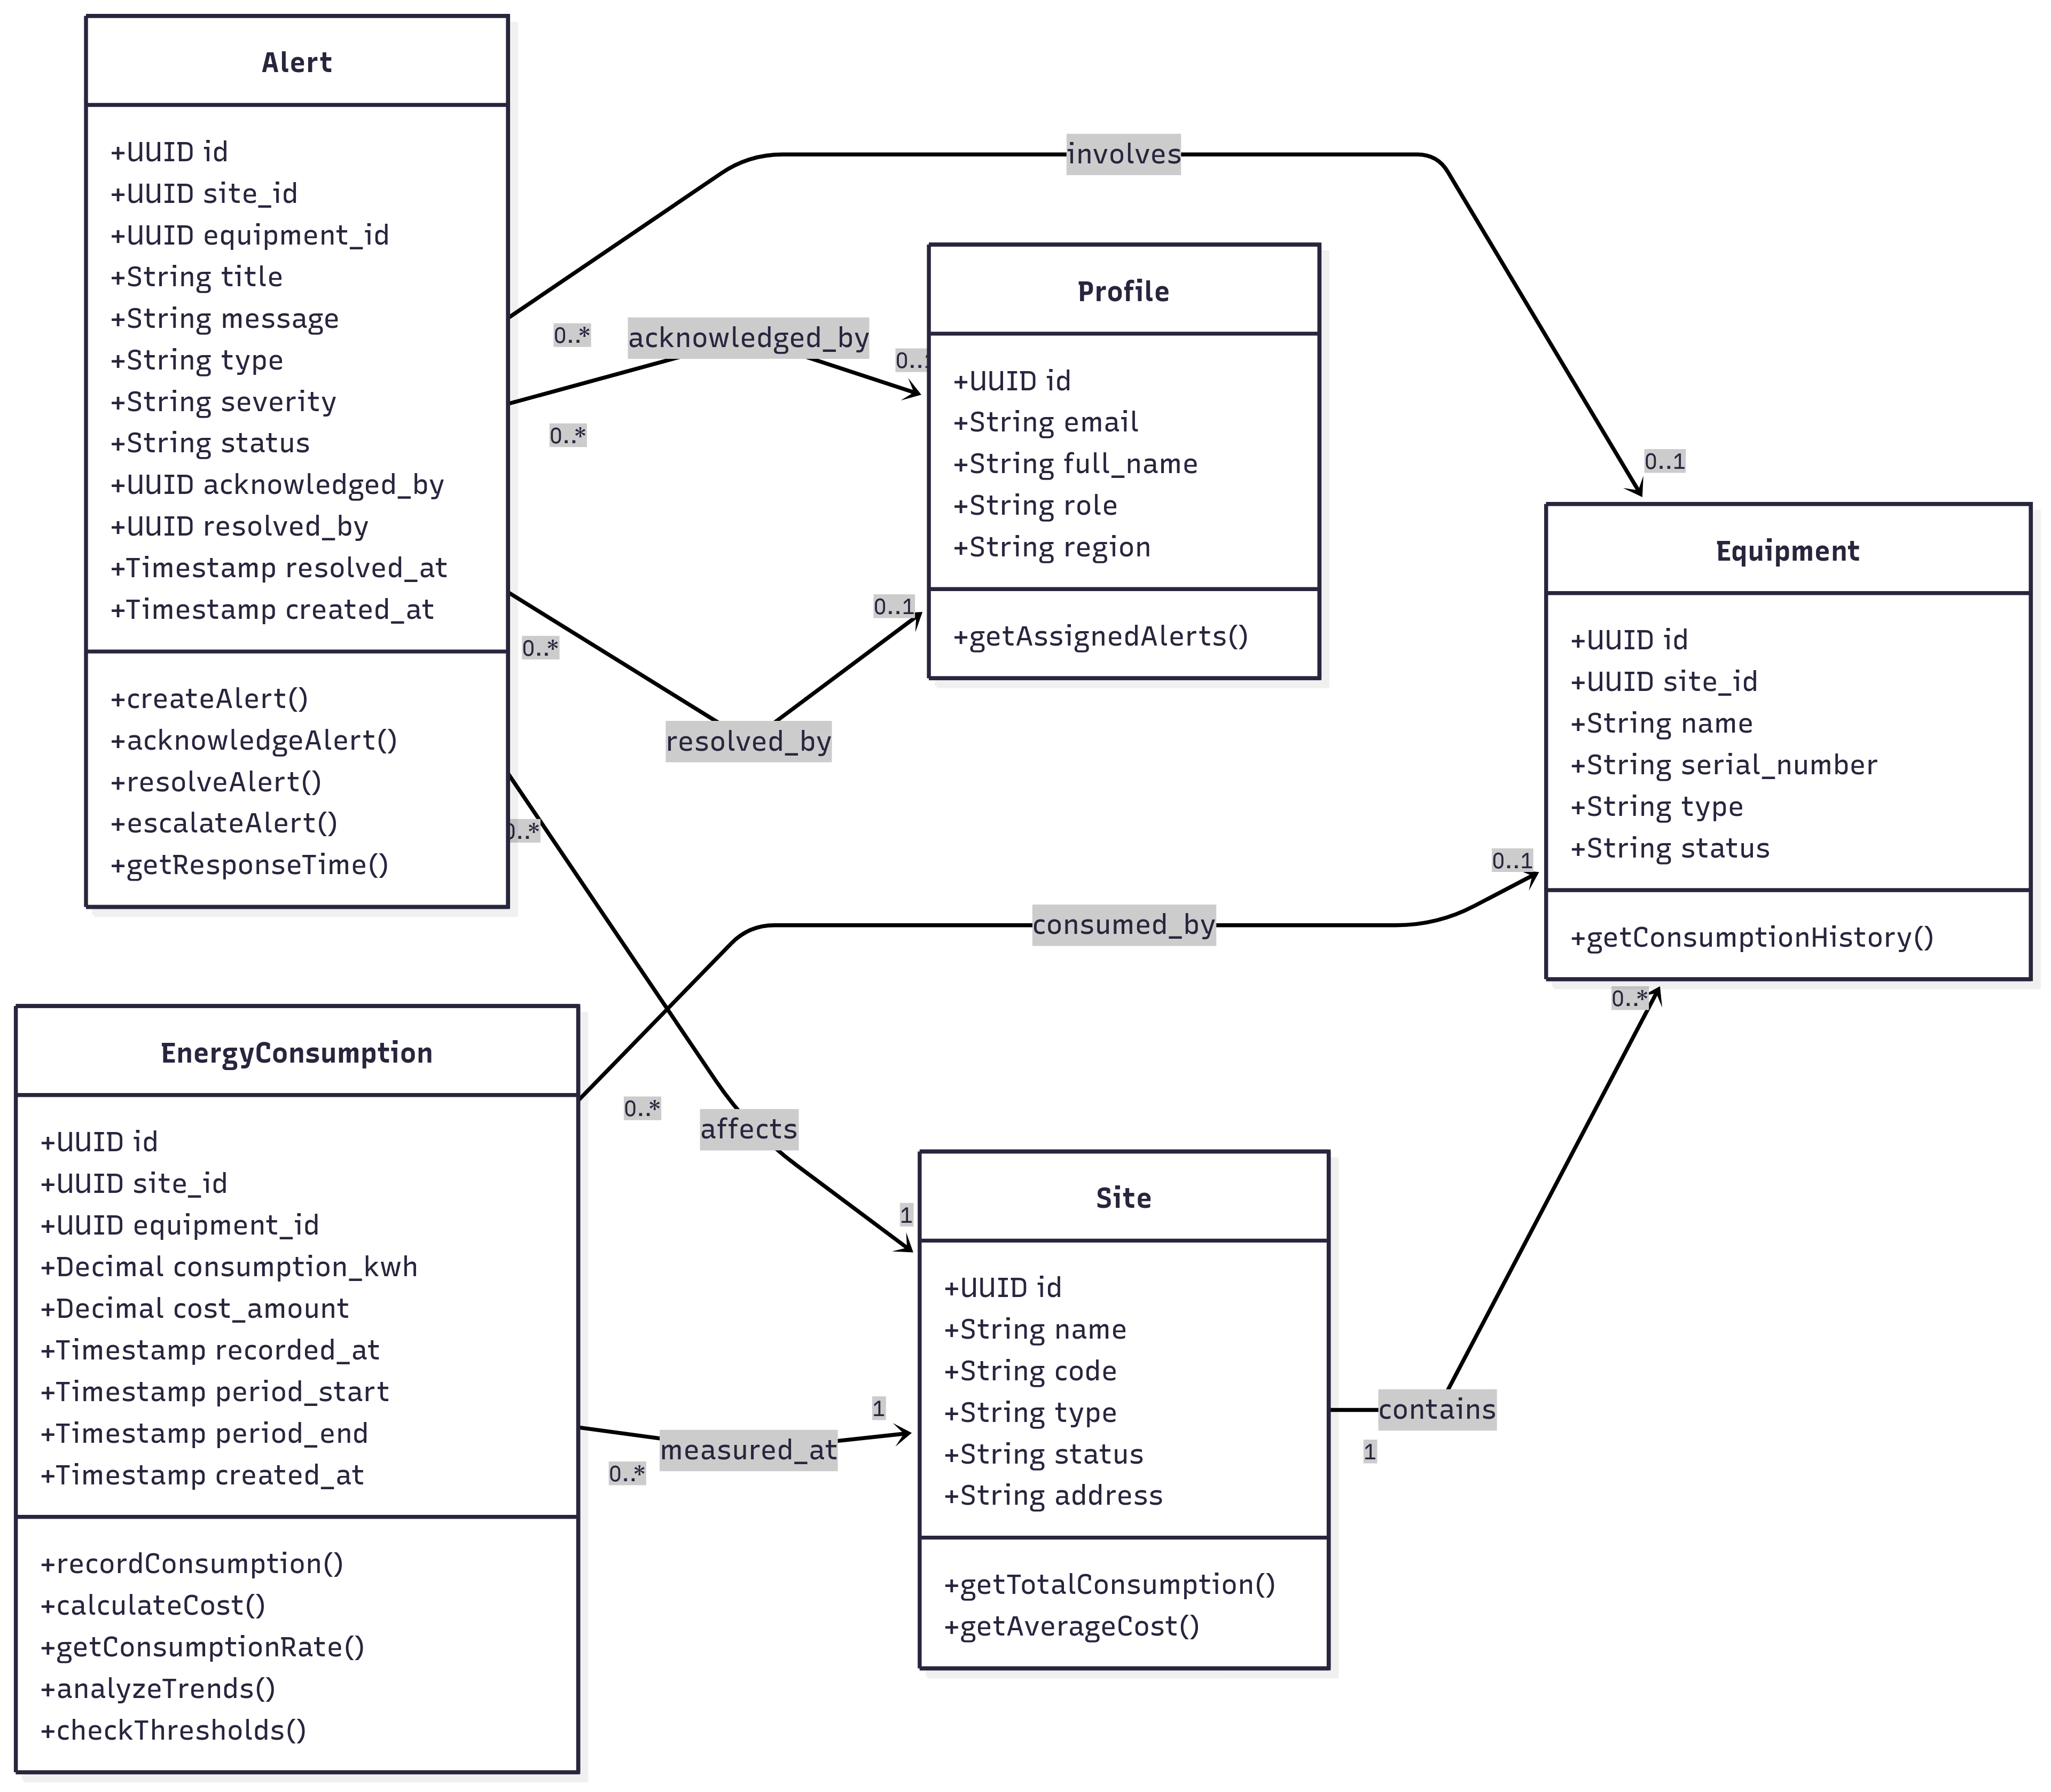
\includegraphics[width=0.7\textwidth]{img/chap_06/class_diagram_sprint4.png}
\caption{Class Diagram - Alert and Energy Consumption Entities}
\end{figure}

The Alert class manages system notifications with attributes for title, message, type, severity, and status. It implements methods for creation, acknowledgment, resolution, and escalation. The EnergyConsumption class captures power usage with consumption in kWh, costs, timestamps, and periods. It supports recording, cost calculation, rate analysis, and threshold validation.

\section{Use Case Diagram}

\begin{figure}[H]
\centering
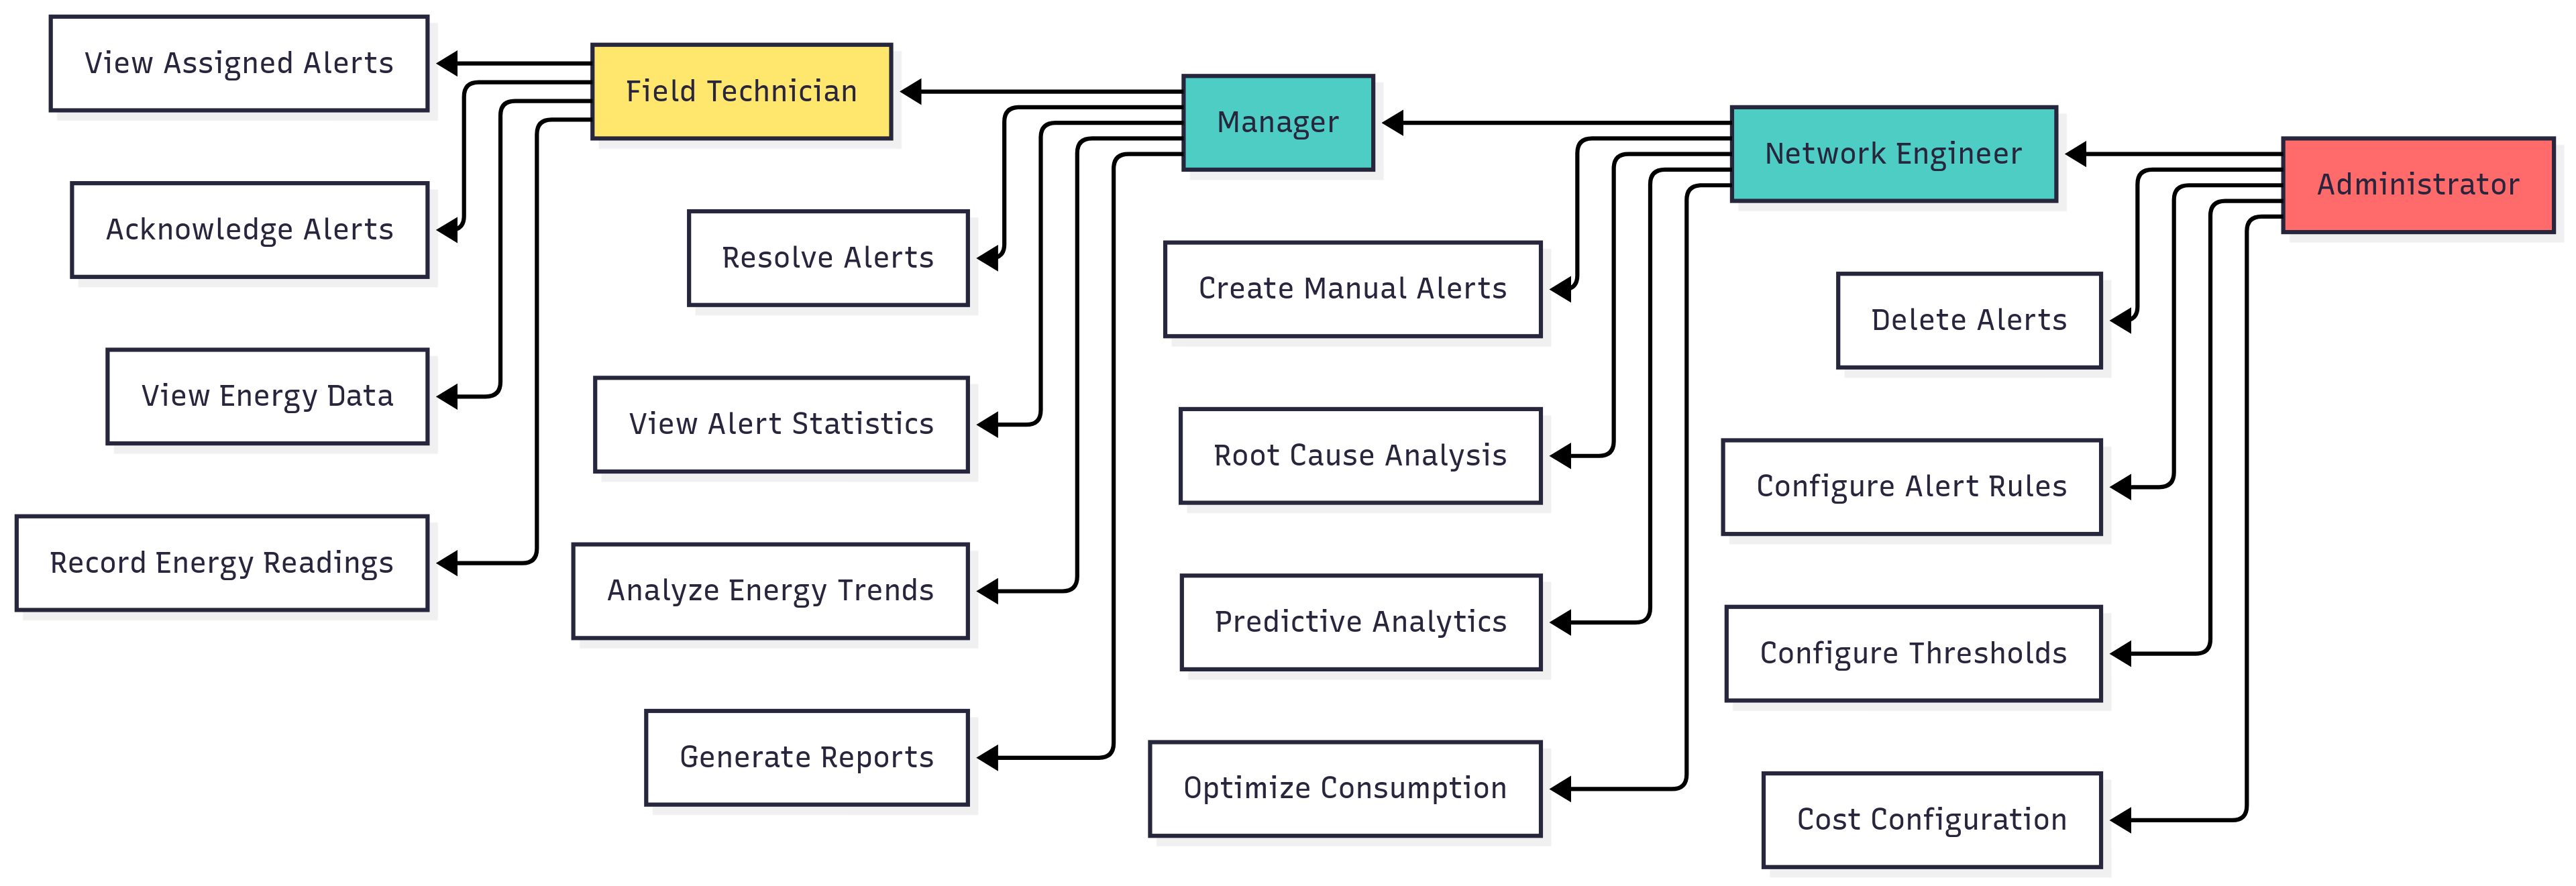
\includegraphics[width=0.7\textwidth]{img/chap_06/usecase_diagram_sprint4.png}
\caption{Use Case Diagram - Role-based Alerts and Energy Management}
\end{figure}

The diagram models role hierarchies: Field Technician has base permissions, Manager extends with alert creation and analysis, Network Engineer adds predictive analytics, and Administrator has complete system control.

\section{Use Case Permissions}

\begin{table}[htbp]
\centering
\caption{Use Case Permissions Matrix}
\small
\begin{tabular}{|p{4.5cm}|c|c|c|c|}
\hline
\textbf{Use Case} & \textbf{Tech} & \textbf{Mgr} & \textbf{Eng} & \textbf{Admin} \\
\hline
View Assigned Alerts & Yes & Yes & Yes & Yes \\
\hline
Acknowledge Alerts & Yes & Yes & Yes & Yes \\
\hline
Resolve Alerts & No & Yes & Yes & Yes \\
\hline
Create Manual Alerts & No & Yes & Yes & Yes \\
\hline
Delete Alerts & No & No & No & Yes \\
\hline
Configure Alert Rules & No & No & No & Yes \\
\hline
View Energy Data & Yes & Yes & Yes & Yes \\
\hline
Record Energy Readings & Yes & Yes & Yes & Yes \\
\hline
Analyze Energy Trends & No & Yes & Yes & Yes \\
\hline
Predictive Analytics & No & No & Yes & Yes \\
\hline
Configure Thresholds & No & No & No & Yes \\
\hline
Generate Reports & No & Yes & Yes & Yes \\
\hline
\end{tabular}
\end{table}

\section{Detailed Use Case: Create Alert}

\begin{table}[htbp]
\centering
\caption{Use Case Description: Create Alert}
\small
\begin{tabular}{|p{3.5cm}|p{10cm}|}
\hline
\textbf{Use Case} & Create System Alert \\
\hline
\textbf{Actors} & Network Engineer, Manager, Administrator \\
\hline
\textbf{Preconditions} & User authenticated with appropriate role. Sites and equipment data available. \\
\hline
\textbf{Main Flow} & 1. User clicks "Create Alert" button, 2. System displays form, 3. User enters title and message, 4. User selects type and severity, 5. User selects site and optional equipment, 6. User submits form, 7. System validates fields, 8. System creates alert with "active" status, 9. System triggers real-time notification, 10. System displays confirmation \\
\hline
\textbf{Alternative Flows} & A1: Validation failure - display errors. A2: Critical alert - send immediate notifications \\
\hline
\textbf{Postconditions} & Alert stored in database. Real-time notification delivered. System log created. \\
\hline
\end{tabular}
\end{table}

\section{Sequence Diagrams}

\begin{figure}[H]
\centering
\begin{minipage}{0.48\textwidth}
\centering
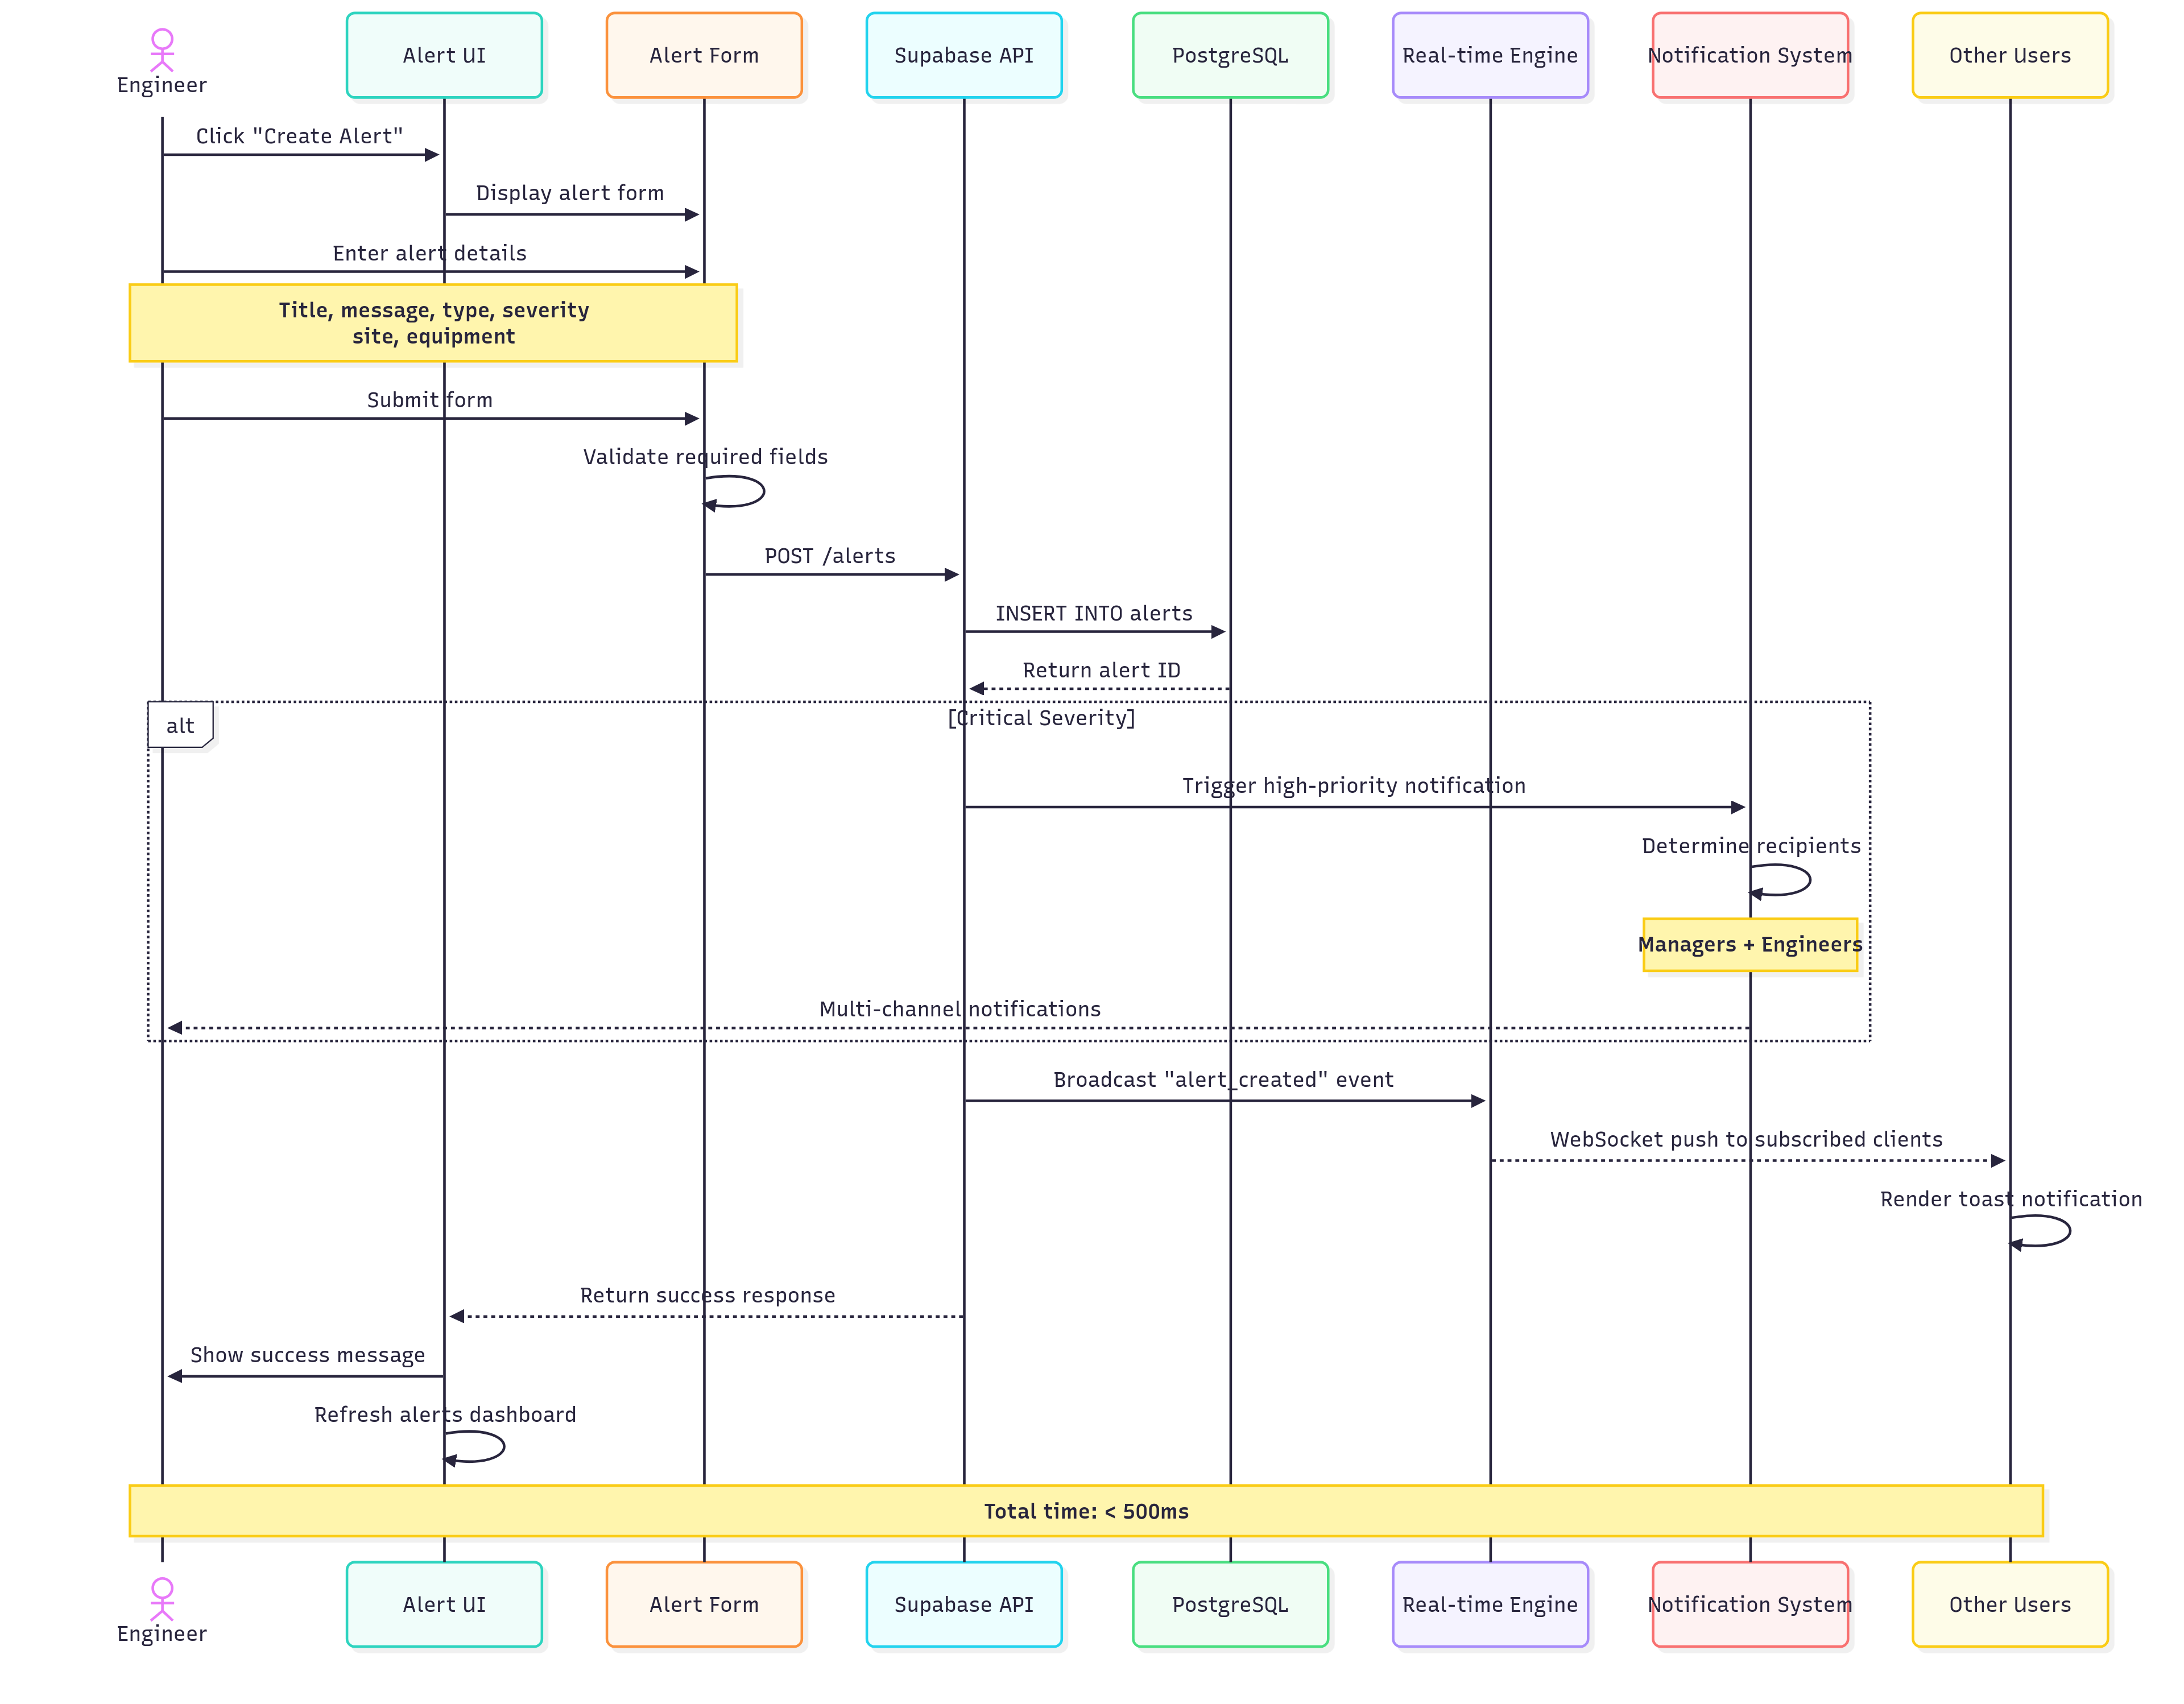
\includegraphics[width=0.95\textwidth]{img/chap_06/sequence_create_alert.png}
\caption{Create Alert Sequence}
\end{minipage}
\hfill
\begin{minipage}{0.48\textwidth}
\centering
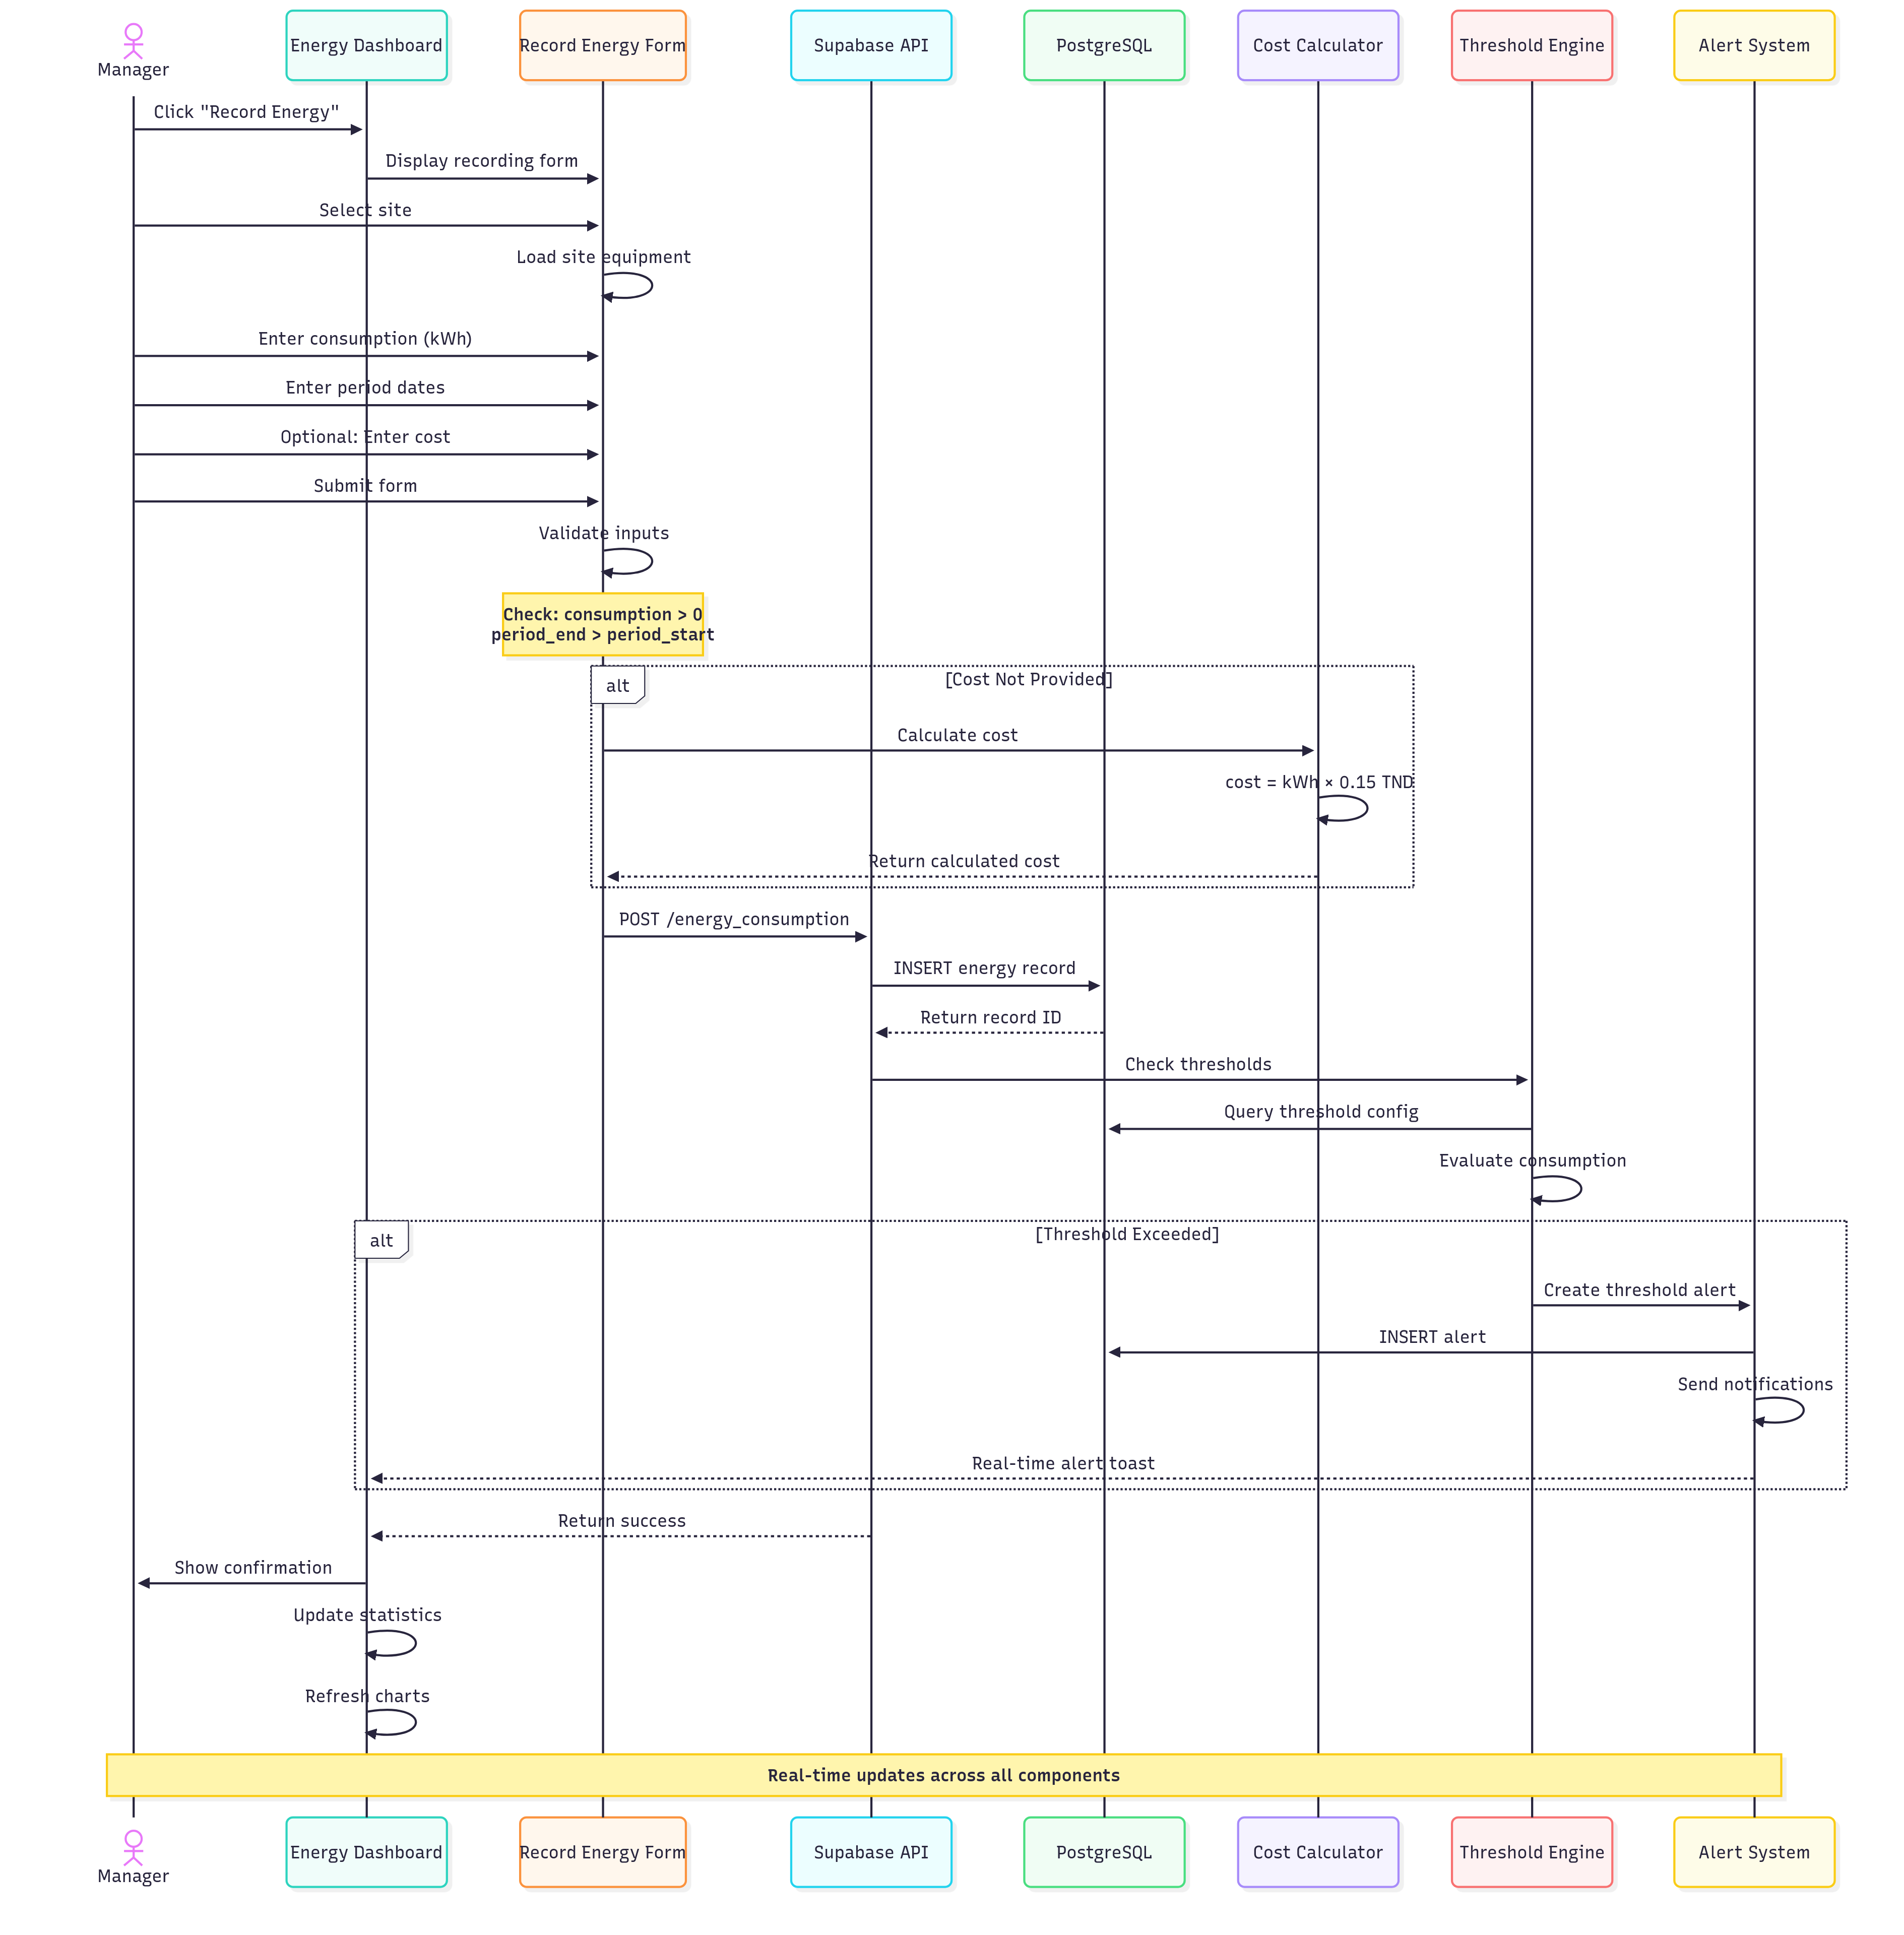
\includegraphics[width=0.95\textwidth]{img/chap_06/sequence_record_energy.png}
\caption{Record Energy Sequence}
\end{minipage}
\end{figure}

The create alert sequence shows: Engineer initiates creation, UI validates and submits to Supabase API, system inserts into PostgreSQL, triggers notifications for critical alerts via Real-time Engine broadcasting WebSocket events to clients. The record energy sequence demonstrates: Manager enters consumption data, Cost Calculator computes cost at 0.15 TND/kWh if not provided, Threshold Engine validates limits and creates alerts if exceeded.

\section{Implementation Screenshots}

\begin{figure}[H]
\centering
\begin{minipage}{0.48\textwidth}
\centering
\fbox{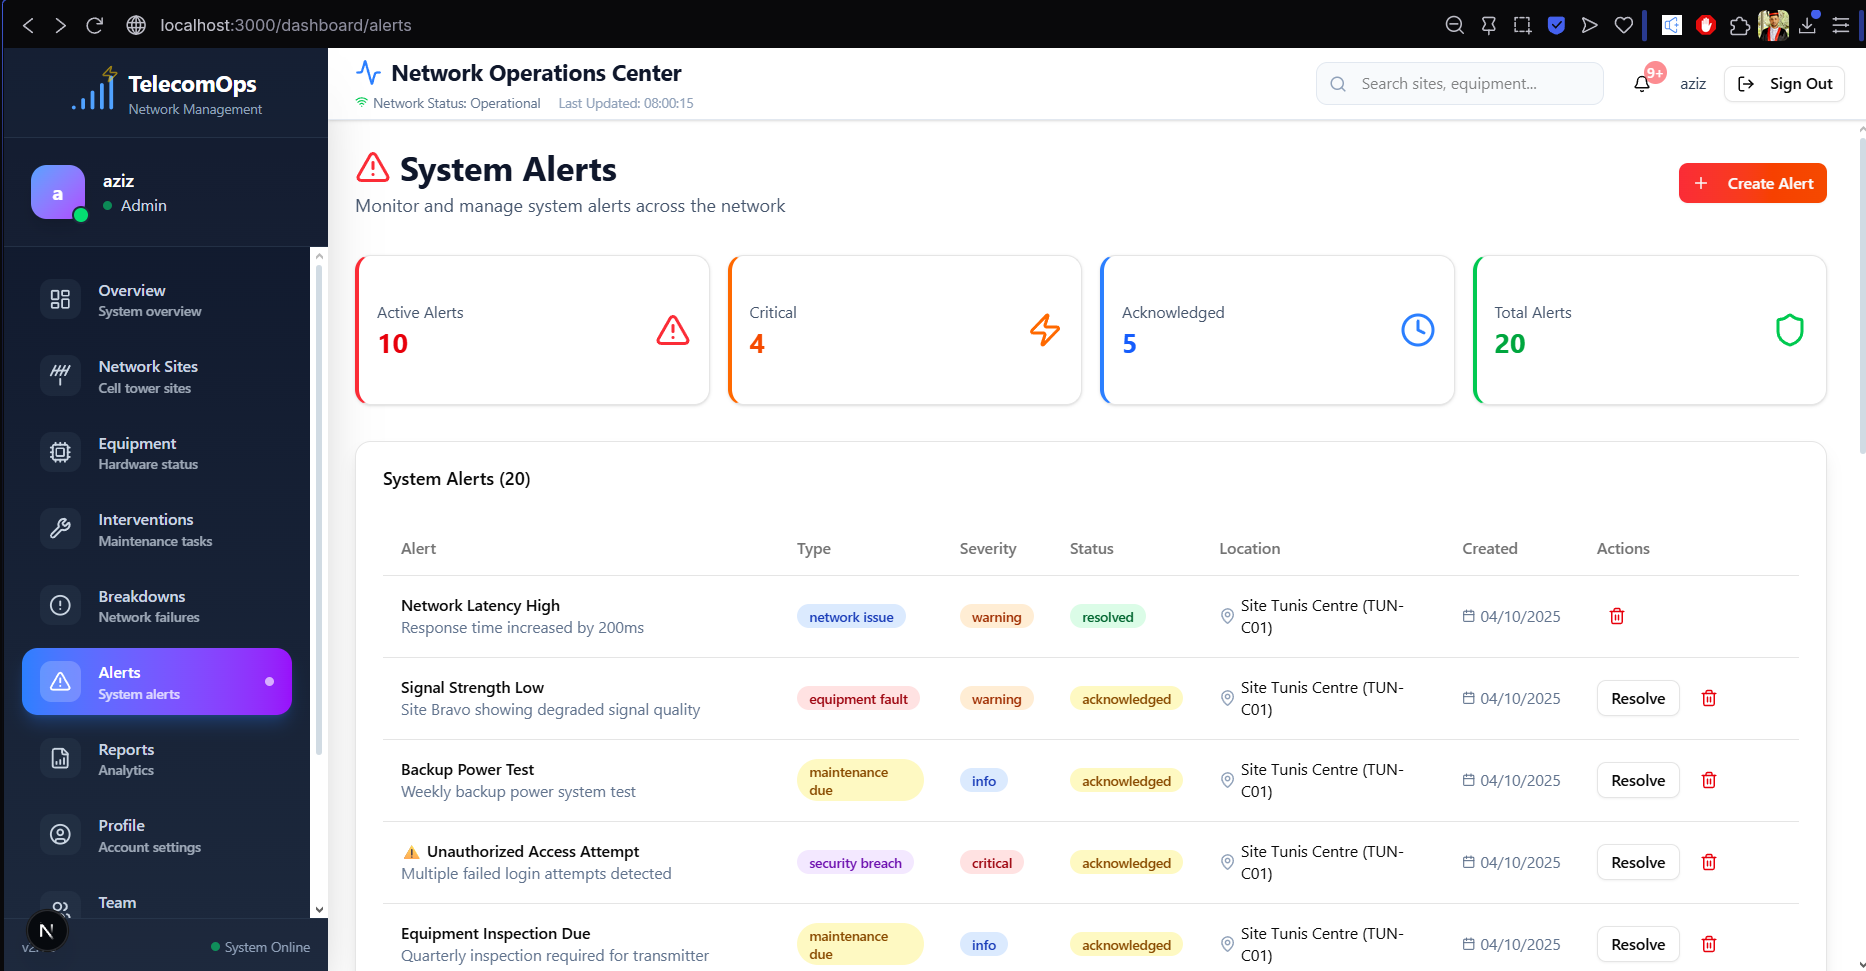
\includegraphics[width=0.95\textwidth]{img/chap_06/screenshot_alerts_dashboard.png}}
\caption{Alerts Dashboard}
\end{minipage}
\hfill
\begin{minipage}{0.48\textwidth}
\centering
\fbox{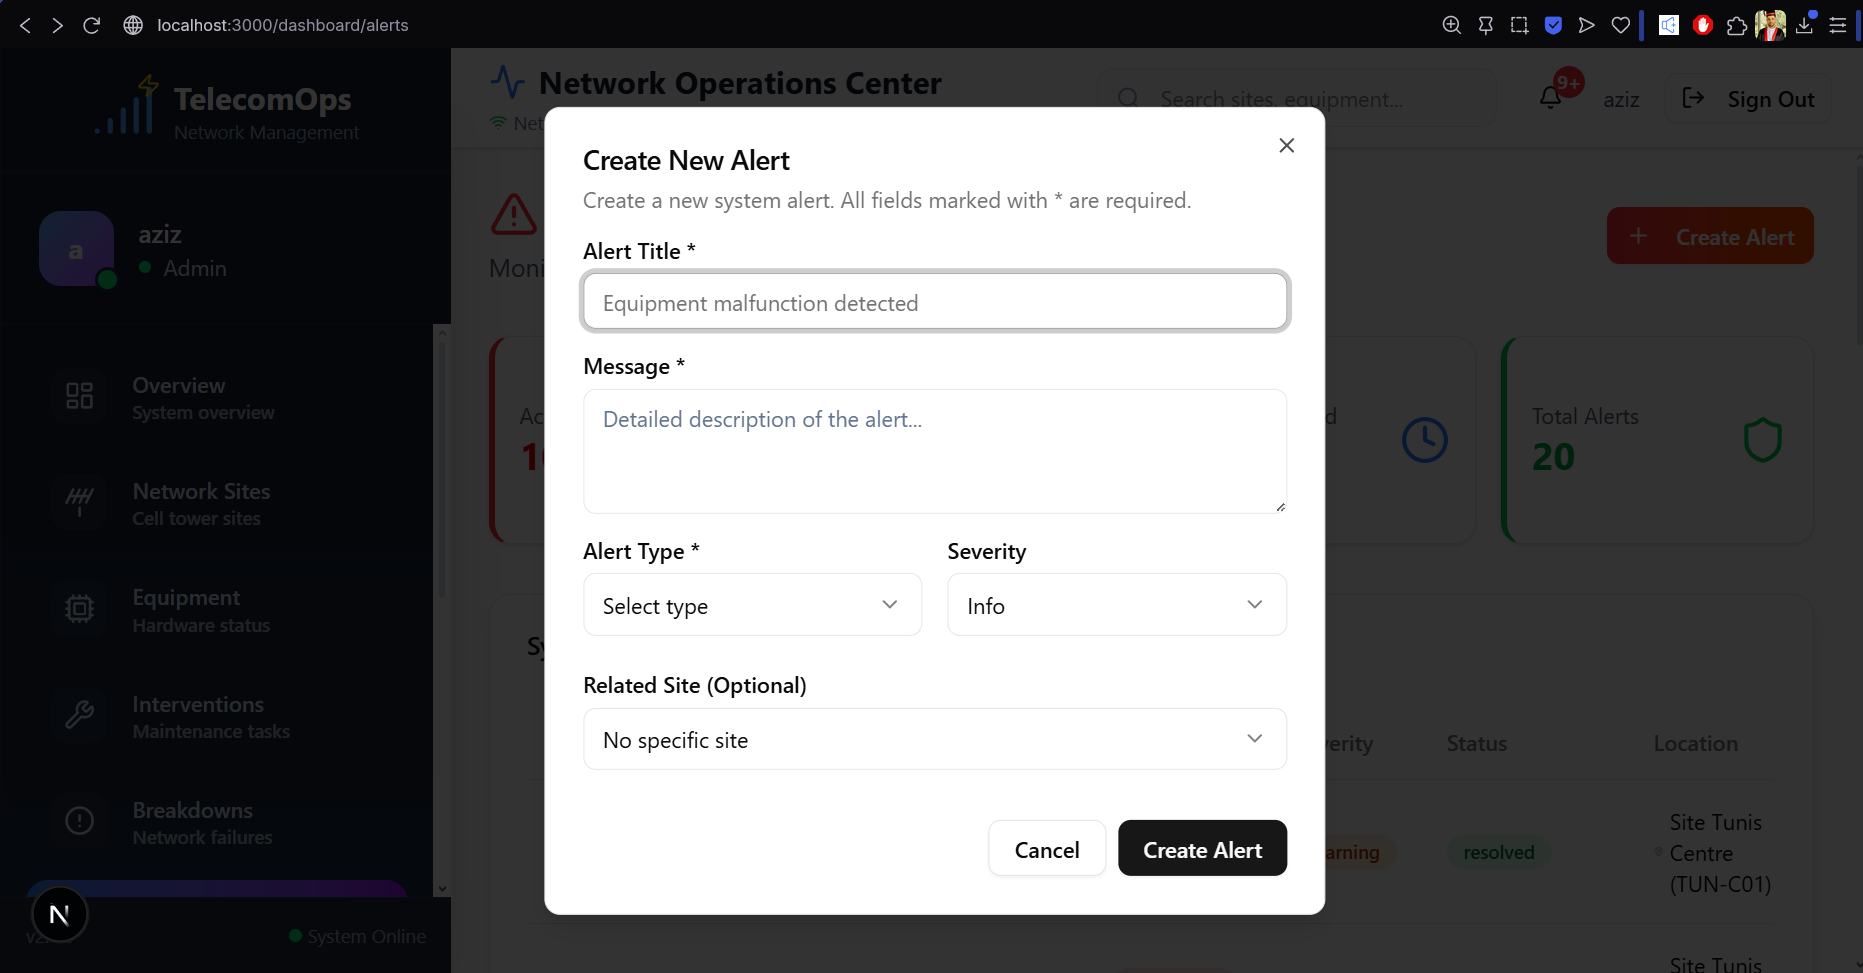
\includegraphics[width=0.95\textwidth]{img/chap_06/screenshot_create_alert.png}}
\caption{Create Alert Dialog}
\end{minipage}
\end{figure}

\begin{figure}[H]
\centering
\begin{minipage}{0.48\textwidth}
\centering
\fbox{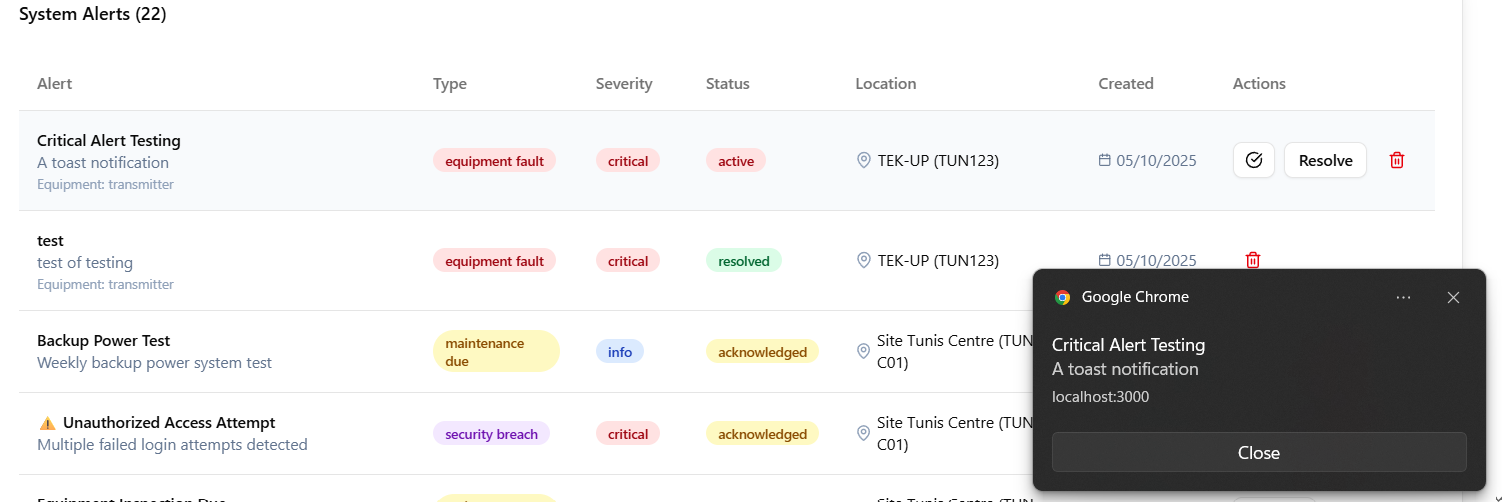
\includegraphics[width=0.95\textwidth]{img/chap_06/screenshot_alert_toast.png}}
\caption{Real-time Notification}
\end{minipage}
\hfill
\begin{minipage}{0.48\textwidth}
\centering
\fbox{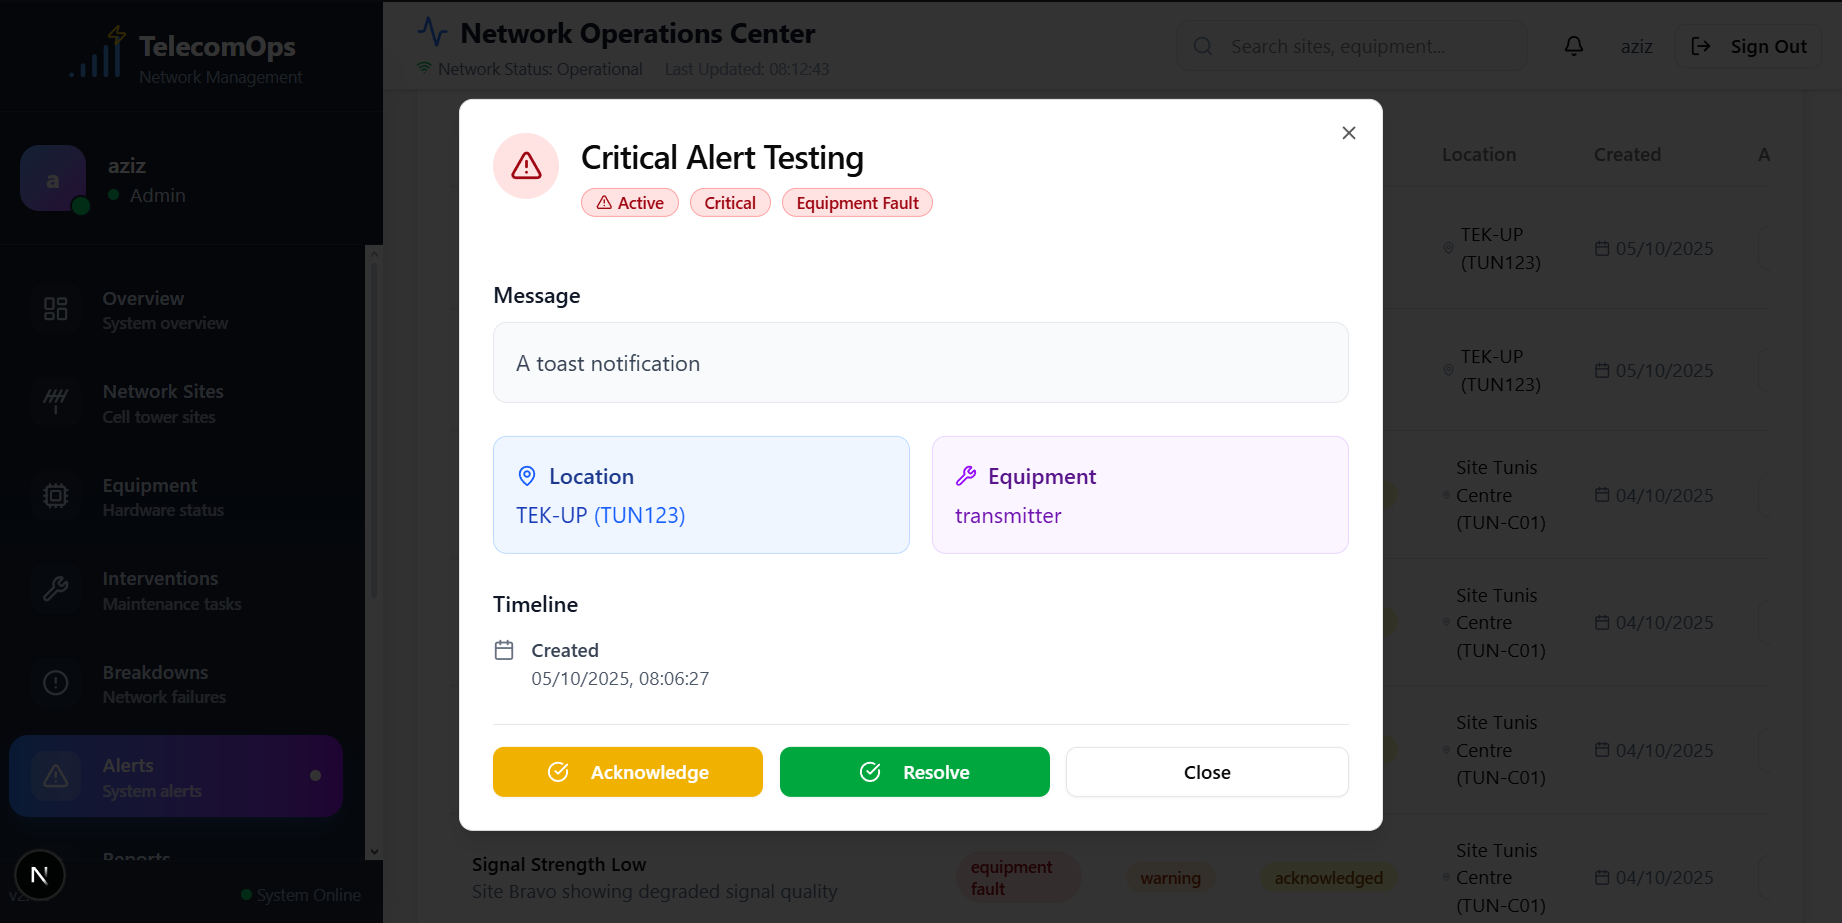
\includegraphics[width=0.95\textwidth]{img/chap_06/screenshot_alert_details.png}}
\caption{Alert Details View}
\end{minipage}
\end{figure}

\begin{figure}[H]
\centering
\begin{minipage}{0.48\textwidth}
\centering
\fbox{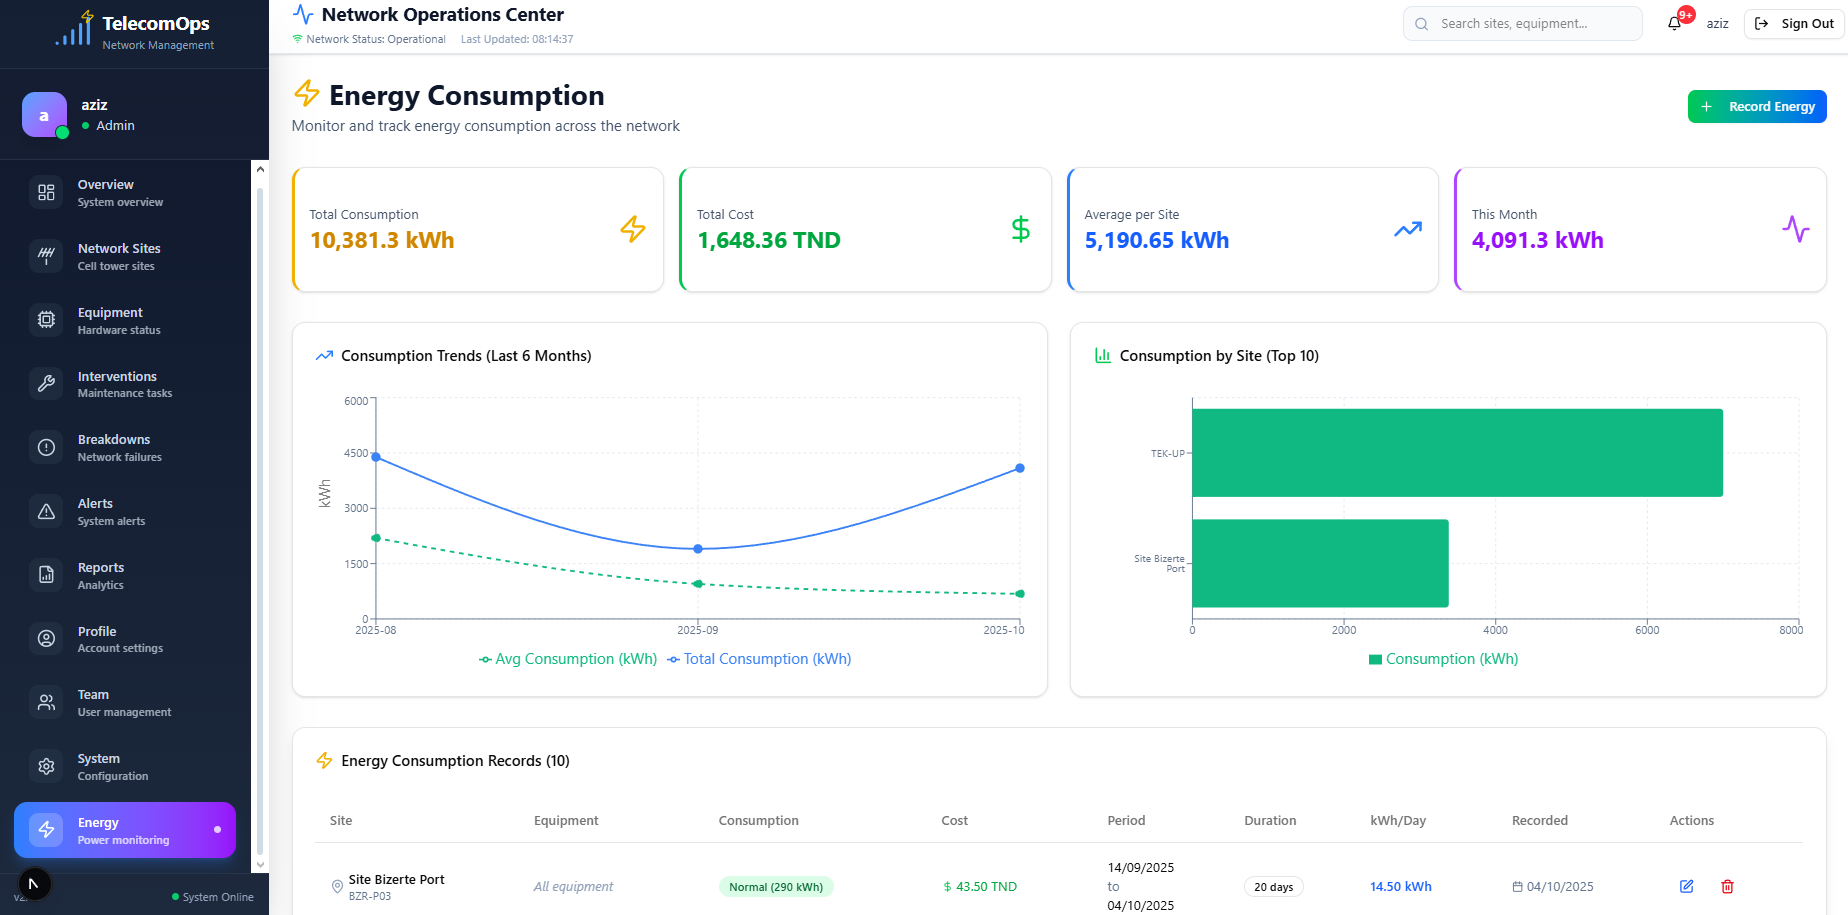
\includegraphics[width=0.95\textwidth]{img/chap_06/screenshot_energy_dashboard.png}}
\caption{Energy Dashboard}
\end{minipage}
\hfill
\begin{minipage}{0.48\textwidth}
\centering
\fbox{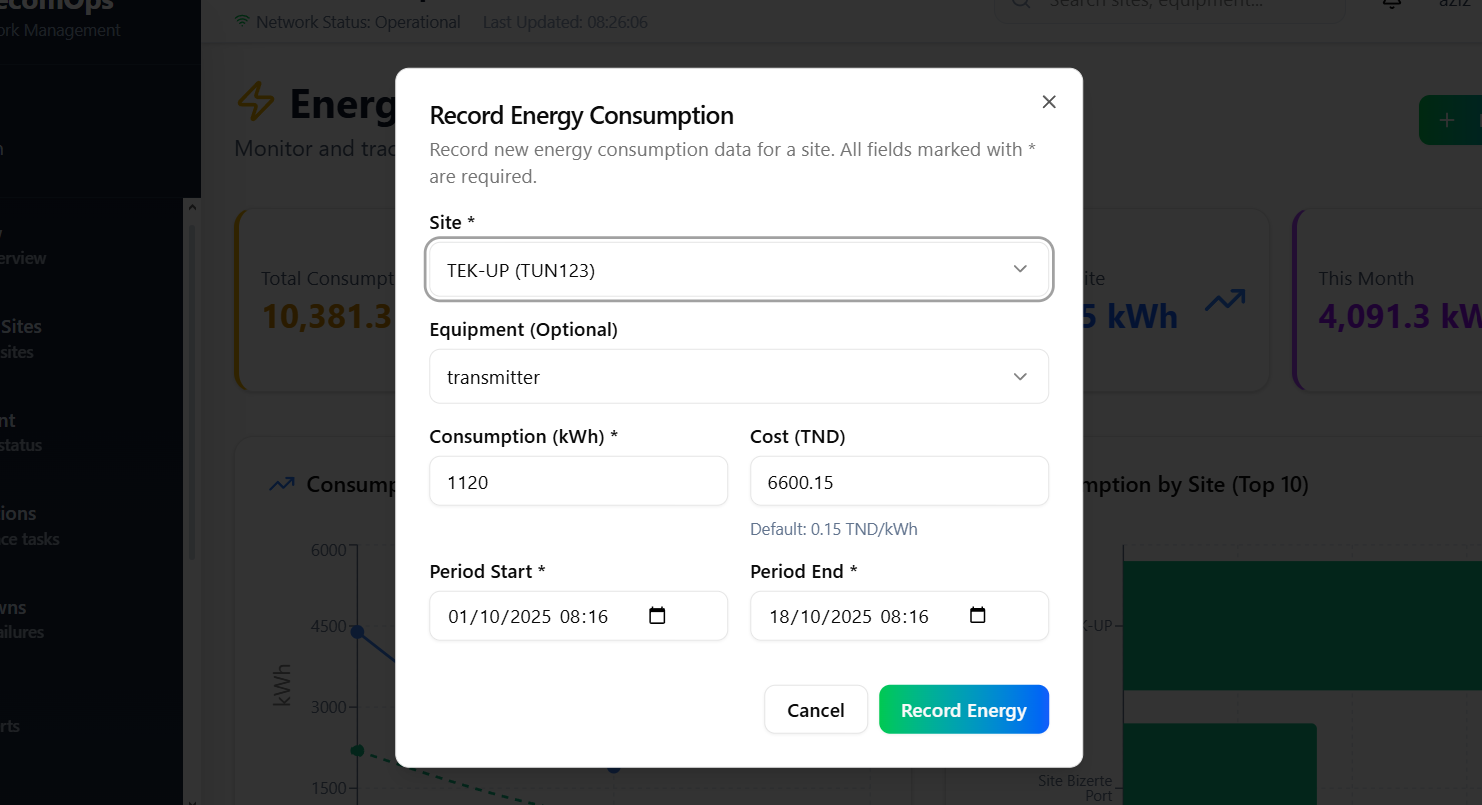
\includegraphics[width=0.95\textwidth]{img/chap_06/screenshot_record_energy.png}}
\caption{Record Energy Dialog}
\end{minipage}
\end{figure}

\begin{figure}[H]
\centering
\begin{minipage}{0.48\textwidth}
\centering
\fbox{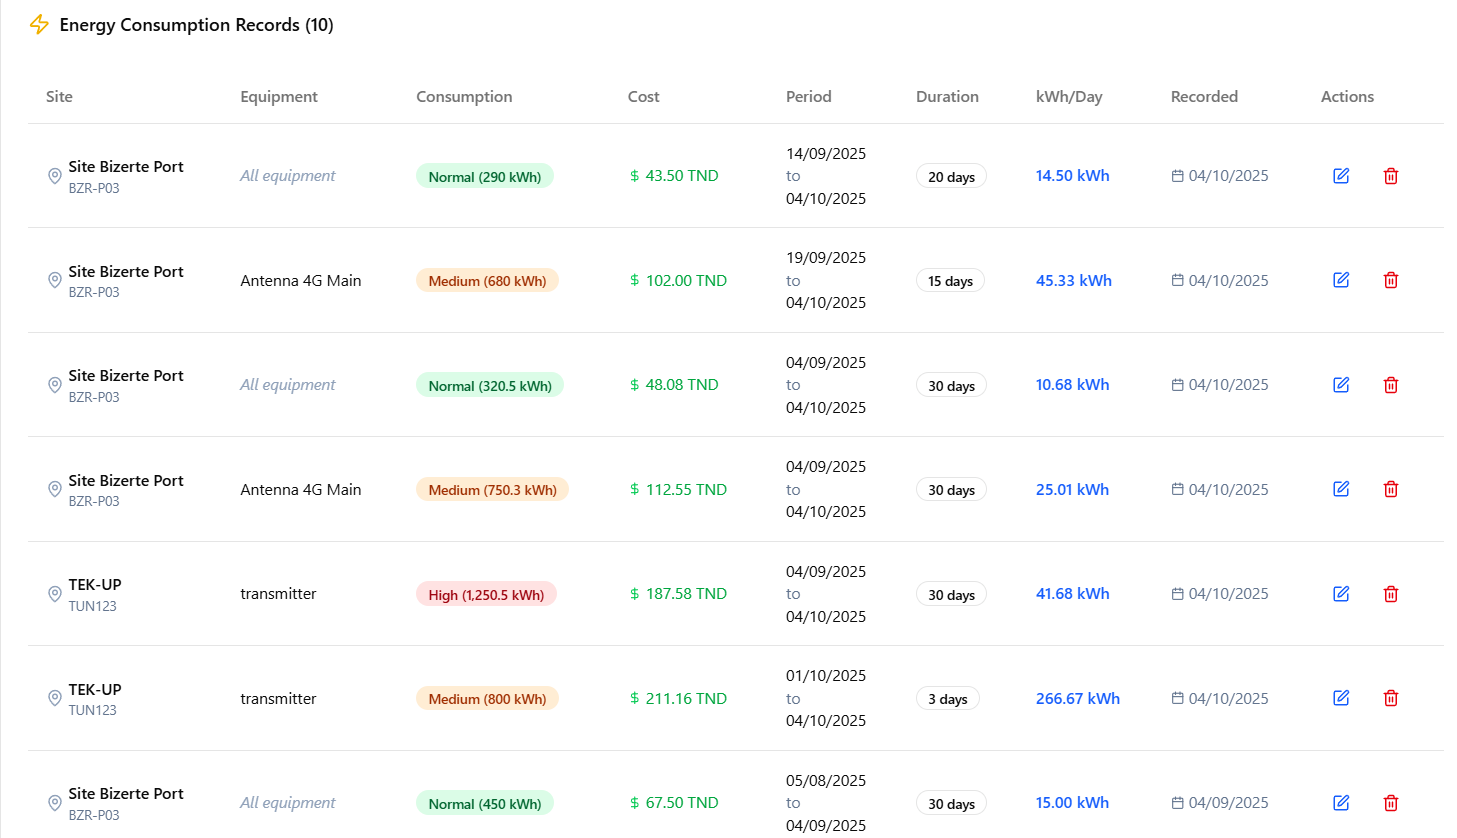
\includegraphics[width=0.95\textwidth]{img/chap_06/screenshot_energy_table.png}}
\caption{Energy Records Table}
\end{minipage}
\hfill
\begin{minipage}{0.48\textwidth}
\centering
\fbox{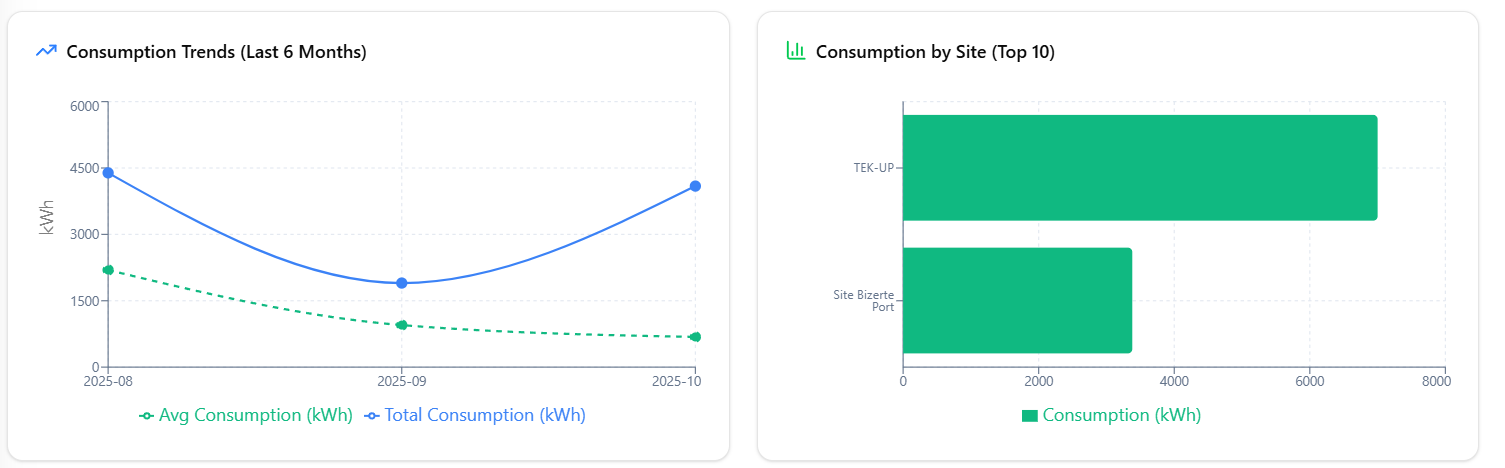
\includegraphics[width=0.95\textwidth]{img/chap_06/screenshot_energy_charts.png}}
\caption{Consumption Charts}
\end{minipage}
\end{figure}

The alerts dashboard displays statistics (active, critical, acknowledged, total) with a comprehensive table showing titles, types, severity, status, and actions. The creation dialog provides validated input for title, message, type, severity, site, and equipment. Real-time toast notifications appear with slide-in animations showing alert details and action buttons. The detail view presents complete information with status-appropriate actions.

The energy dashboard shows statistics (total kWh, cost, average, monthly) with trend charts. The record dialog includes site/equipment selection, kWh input, automatic cost calculation at 0.15 TND/kWh, and period validation. The table displays color-coded consumption (red >1000, orange 500-1000, green <500 kWh), costs, duration, and daily rates. Charts show 6-month trends and top 10 sites comparison.

\section{Technical Challenges and Solutions}

\subsection{Real-time Alert Notifications}

\textbf{Challenge:} Implementing scalable real-time notifications with minimal latency across distributed sessions.

\textbf{Solution:} The system uses Supabase WebSocket subscriptions for bidirectional communication. Critical alerts broadcast events to subscribed clients via the Real-time Engine. The AlertNotificationToast component maintains persistent connections with automatic reconnection logic and exponential backoff. This achieves 200ms delivery latency while supporting concurrent sessions through connection pooling and server-side event filtering.

\subsection{Energy Cost Auto-calculation}

\textbf{Challenge:} Flexible cost calculation supporting automatic rates and manual overrides for varying pricing models.

\textbf{Solution:} The Cost Calculator implements dual-mode calculation: automatic mode multiplies kWh by configured rate (0.15 TND/kWh), manual override allows custom costs. Client-side calculation provides immediate feedback, server-side ensures integrity. The system stores calculated cost and override flag, with centralized rate configuration accessible only to administrators. Historical data remains unchanged when rates update.

\subsection{Consumption Analytics Aggregation}

\textbf{Challenge:} Efficiently aggregating large consumption datasets while providing real-time analytics and optimized rendering.

\textbf{Solution:} PostgreSQL materialized views pre-compute monthly/daily aggregations with incremental refresh. Dashboard queries use views instead of raw records. SQL window functions enable efficient trend calculation. The 6-month chart uses date truncation and GROUP BY, top 10 query employs RANK() with LIMIT. React Query caching stores results with 5-minute TTL. Redis provides sub-100ms response for high-traffic analytics.

\section{Testing and Validation}

\subsection{Functional Testing}

Alert tests validate field validation, type/severity selection, site/equipment association, status transitions, user tracking, and timestamp accuracy. Notification tests verify delivery, toast rendering, auto-dismiss (10s), and manual dismiss. Energy tests validate numeric input, cost calculation accuracy, date validation, and equipment handling. Chart tests confirm data accuracy, aggregation, scaling, and tooltips. Threshold tests verify limit comparison and automatic alert generation.

\subsection{Integration Testing}

Database tests verify Supabase connectivity, Row-Level Security enforcement, foreign key constraints, and transaction integrity. Real-time tests confirm WebSocket establishment, event broadcasting, automatic reconnection, and message ordering. Authentication tests validate role-based access, JWT validation, session management, and unauthorized access prevention. Form tests verify cascading dropdowns, validation consistency, error propagation, and optimistic updates with rollback.

\subsection{Performance Testing}

Alert performance: creation <300ms, notification <200ms, dashboard load <2s (1000+ alerts), 100+ concurrent users. Energy performance: calculation accuracy under load, chart rendering <1s (1000+ points), query <500ms, export optimization. Load tests: 500 concurrent alert creations, 1000 notifications/minute, 10,000 energy queries, 1000 DB ops/second. Memory profiling optimizes heap usage, WebSocket overhead, and React re-renders. Results show linear scaling to 1000 users with under 5 percent degradation.

\section{Conclusion}

Sprint 4 successfully delivers critical systems enhancing TelecomOps capabilities. The Alerts Management System provides incident tracking with sub-200ms real-time notifications via WebSocket architecture, supporting automated/manual creation, role-based workflow, and complete audit trails. The Energy Consumption Monitoring System enables data-driven management with automatic cost calculation, visual analytics, and threshold alerting, processing data efficiently through materialized views with under 1-second dashboard rendering.

Technical achievements include scalable real-time architecture (1000+ sessions), flexible cost calculation with overrides, and high-performance analytics with multi-layered aggregation. Future enhancements will add ML-based anomaly detection, predictive alerting, automated resolution recommendations, comparative site analytics, consumption modeling, and external system integration for advanced operations management and sustainability initiatives.
        \clearpage
        
        \newpage

\chapter{Sprint 5: Reporting and Analytics Dashboard}

\cfoot{\thepage}

\parindent=0.5in
\onehalfspacing

\section{Introduction}

Sprint 5, titled "Reporting and Analytics Dashboard," implements comprehensive reporting and analytics capabilities enabling data-driven decision making through intelligent visualization, flexible filtering, and multi-format export functionality. This sprint addresses user stories US-012 (Analytics Dashboard), US-013 (Custom Reports), and US-014 (Data Export) from Chapter 2's product backlog.

Network operations generate massive data volumes across sites, equipment, maintenance activities, incidents, and alerts established in Sprints 1-4. The reporting system aggregates this data presenting unified views of network health, operational efficiency, and service quality metrics supporting the stakeholder requirements identified in Chapter 2.

Advanced visualization techniques including interactive charts, trend analysis, and comparative statistics enable stakeholders to identify patterns, detect anomalies, and make informed decisions. The implementation leverages data from all previous sprints providing comprehensive operational intelligence.

\section{Sprint Backlog}

During sprint planning, we defined the tasks required for Sprint 5 implementation. Table 7.1 presents the sprint backlog with user stories, tasks, complexity assessments, and effort estimates.

\begin{table}[H]
\centering
\small
\begin{tabular}{|p{2.5cm}|p{4cm}|p{3.2cm}|p{2.2cm}|p{1.5cm}|}
\hline
\textbf{Functionality} & \textbf{User Story} & \textbf{Tasks} & \textbf{Complexity} & \textbf{Estimate} \\
\hline

\multirow{3}{2.5cm}{Analytics Dashboard (US-012)} & 
\multirow{3}{4cm}{As manager, I want comprehensive analytics dashboard for operations overview}
& Create dashboard layout & Medium & 3h \\
\cline{3-5}
& & Aggregate statistics & Hard & 3h \\
\cline{3-5}
& & Implement KPIs & Medium & 2h \\
\hline

\multirow{3}{2.5cm}{Interactive Charts} & 
\multirow{3}{4cm}{As engineer, I want interactive charts for data visualization}
& Implement chart components & Medium & 3h \\
\cline{3-5}
& & Add filtering capability & Medium & 2h \\
\cline{3-5}
& & Enable drill-down & Hard & 2h \\
\hline

\multirow{3}{2.5cm}{Custom Reports (US-013)} & 
\multirow{3}{4cm}{As manager, I want to generate custom reports with date ranges}
& Create report builder & Medium & 3h \\
\cline{3-5}
& & Implement date filters & Easy & 2h \\
\cline{3-5}
& & Add preset options & Easy & 1h \\
\hline

\multirow{3}{2.5cm}{Breakdown Analysis} & 
\multirow{3}{4cm}{As engineer, I want detailed breakdown analysis with metrics}
& Calculate MTTR/MTBF & Hard & 3h \\
\cline{3-5}
& & Show impact analysis & Medium & 2h \\
\cline{3-5}
& & Create analysis view & Easy & 1h \\
\hline

\multirow{3}{2.5cm}{Export CSV (US-014)} & 
\multirow{3}{4cm}{As manager, I want to export reports to CSV format}
& Implement CSV generation & Medium & 2h \\
\cline{3-5}
& & Handle large datasets & Medium & 2h \\
\cline{3-5}
& & Optimize encoding & Easy & 1h \\
\hline

\multirow{3}{2.5cm}{Export PDF (US-014)} & 
\multirow{3}{4cm}{As admin, I want to export reports to PDF format}
& Implement PDF with jsPDF & Hard & 3h \\
\cline{3-5}
& & Add progress tracking & Medium & 2h \\
\cline{3-5}
& & Format multi-page layout & Medium & 2h \\
\hline

\multirow{3}{2.5cm}{Performance KPIs} & 
\multirow{3}{4cm}{As manager, I want to view key performance indicators}
& Calculate uptime metrics & Medium & 2h \\
\cline{3-5}
& & Calculate response time & Medium & 2h \\
\cline{3-5}
& & Calculate efficiency metrics & Easy & 1h \\
\hline

\multirow{3}{2.5cm}{Date Range Filter} & 
\multirow{3}{4cm}{As user, I want to filter reports by date period}
& Implement date picker & Easy & 2h \\
\cline{3-5}
& & Add preset shortcuts & Easy & 2h \\
\cline{3-5}
& & Add custom range & Medium & 2h \\
\hline

\end{tabular}
\caption{Sprint 5 Backlog with Task Breakdown}
\label{tab:sprint5_backlog}
\end{table}

The backlog totals 50 hours across eight major functionalities. PDF generation complexity stems from client-side rendering requirements and memory management. Data aggregation requires efficient query optimization processing thousands of historical records from Sprints 2-4.

\section{Conceptual Design}

This section presents the conceptual design models guiding Sprint 5 implementation.

\subsection{Class Diagram}

Figure 7.1 presents the class diagram illustrating the reporting system architecture integrating data from all previous sprints.

\begin{figure}[H]
    \centering
    \includegraphics[width=0.95\linewidth]{img/chap_07/sprint5_class_diagram.png}
    \caption{Class Diagram - Reporting and Analytics System}
    \label{fig:class_diagram_sprint5}
\end{figure}

The class diagram (Figure 7.1) illustrates the reporting architecture aggregating data from Site, Equipment, Intervention, Breakdown, Alert, and EnergyConsumption entities established in previous sprints.

The ReportGenerator class creates various report types including network summary aggregating site and equipment data from Sprint 1 and 2, equipment status reports, maintenance history from Sprint 3, and breakdown analysis. The class supports flexible date range selection, customizable filtering, and multiple output formats.

The Analytics class calculates key performance indicators including network uptime percentage, Mean Time To Repair (MTTR) from breakdown data, Mean Time Between Failures (MTBF) from equipment history, and response time metrics from intervention tracking. These calculations leverage the comprehensive operational data collected throughout all sprints.

The ChartBuilder transforms aggregated data into visualization formats supporting line charts for trends, bar charts for comparisons, pie charts for distributions, and area charts for cumulative metrics. The ExportManager handles data export in CSV, JSON, and PDF formats with proper encoding and formatting.

\subsection{Use Case Diagram}

Figure 7.2 presents the use case diagram showing role-based permissions for reporting functionality, following the inheritance hierarchy established in Chapter 3.

\begin{figure}[H]
    \centering
    \includegraphics[width=0.45\linewidth]{img/chap_07/sprint5_usecase_diagram.png}
    \caption{Use Case Diagram - Sprint 5 with Role Inheritance}
    \label{fig:use_case_diagram_sprint5}
\end{figure}

The use case diagram (Figure 7.2) demonstrates the established role inheritance hierarchy. Field Technicians access basic reports showing personal performance metrics and assigned tasks. Managers inherit all technician capabilities while adding team reports, departmental analytics, and CSV export for data sharing. Network Engineers inherit all manager capabilities while adding technical reports, root cause analysis capabilities, and custom filtering for detailed investigation. Administrators inherit all engineer capabilities while possessing executive dashboards, PDF export for formal reporting, and report scheduling capabilities.

\textbf{Use Case Description: Generate Report}

Table 7.2 provides detailed information on the "Generate Report" use case as representative of Sprint 5 reporting functionality.

\begin{table}[H]
\centering
\small
\begin{tabular}{|p{3cm}|p{8.5cm}|}
\hline
\textbf{Element} & \textbf{Description} \\
\hline
\textbf{Use Case Name} & Generate Report \\
\hline
\textbf{Primary Actors} & Network Engineer, Operations Manager, Administrator \\
\hline
\textbf{Description} & Generate comprehensive reports aggregating operational data across selected time periods with customizable filtering \\
\hline
\textbf{Pre-condition} & User authenticated with appropriate role; Historical data available from Sprints 1-4; Aggregation services operational \\
\hline
\textbf{Post-condition} & Report generated and displayed; Export options available; Activity logged for audit \\
\hline
\textbf{Main Scenario} & 
1. User navigates to reports dashboard
2. User selects report type (network, equipment, maintenance, breakdown)
3. User sets date range using presets or custom selection
4. User applies optional filters (site, severity, status)
5. User clicks "Generate Report" button
6. System validates parameters
7. System aggregates data from multiple tables
8. System calculates performance metrics
9. System generates visualizations
10. System displays complete report
11. System enables export options
\\
\hline
\textbf{Alternative Flows} & 
A1 - PDF Export: User selects "Export PDF", system shows progress tracking through five stages, generates PDF with proper formatting, triggers download when complete
A2 - Preset Selection: User selects quick preset (Last 7 Days, Last 30 Days), system auto-fills date range
\\
\hline
\textbf{Exception Scenarios} & 
E1: Insufficient data for selected period → Display warning with alternative suggestions
E2: Large dataset exceeds memory → Initiate background processing with email notification
E3: Export failure → Log error details and offer retry options
\\
\hline
\end{tabular}
\caption{Detailed Use Case Description - Generate Report}
\label{tab:generate_report_usecase}
\end{table}

\section{Sequence Diagrams}

This section presents sequence diagrams detailing the main processes implemented in Sprint 5.

\subsection{Generate Report Process}

Figure 7.3 demonstrates the complete workflow for generating analytical reports with data aggregation from multiple sources.

\begin{figure}[H]
    \centering
    \includegraphics[width=0.95\linewidth]{img/chap_07/sprint5_sequence_report.png}
    \caption{Sequence Diagram - Generate Report Process}
    \label{fig:sequence_generate_report}
\end{figure}

\textbf{Note on Sequence Diagram:} Following UML sequence diagram standards, return messages should use dashed arrows (-->) while request messages use solid arrows (->), clearly distinguishing between calls and responses.

The generate report sequence (Figure 7.3) demonstrates the workflow for creating analytical reports. An authorized user navigates to the reports dashboard and selects desired report type (network summary, equipment status, maintenance history, or breakdown analysis). The user configures the report by setting date range using quick presets or custom selection, applying optional filters for specific sites or equipment, and selecting visualization preferences.

Upon clicking "Generate Report", the system validates parameters ensuring dates are logical and filters are compatible. The ReportGenerator component queries multiple data sources including sites table from Sprint 1, equipment records from Sprint 2, interventions and breakdowns from Sprint 3, and alerts and energy data from Sprint 4. The Analytics engine calculates key performance indicators including uptime percentage, MTTR, MTBF, and efficiency metrics. The ChartBuilder transforms aggregated data into visualization components. The complete report displays with interactive charts, summary statistics, and detailed tables.

\subsection{Export Data Process}

Figure 7.4 illustrates the workflow for exporting report data to CSV, JSON, and PDF formats.

\begin{figure}[H]
    \centering
    \includegraphics[width=0.95\linewidth]{img/chap_07/sprint5_sequence_export.png}
    \caption{Sequence Diagram - Export Data Process}
    \label{fig:sequence_export_data}
\end{figure}

The export data sequence (Figure 7.4) demonstrates multi-format export capabilities. When a user selects export format (CSV, JSON, or PDF), the ExportManager validates the request ensuring appropriate permissions. For CSV export, the system serializes tabular data with proper encoding and triggers immediate download. For JSON export, the system structures hierarchical data with metadata and initiates download.

For PDF export, the process is more complex due to client-side generation constraints. The system initializes jsPDF library, creates staged generation with five phases (preparation, summary, metrics, breakdowns, finalization), updates progress bar showing 0-100% completion, formats multi-page layout with headers and footers, and triggers download when complete. Progress tracking provides user feedback during generation preventing perceived freezing.

\section{Implementation}

This section presents screenshots illustrating the interfaces developed during Sprint 5 implementation.

\subsection{Analytics Dashboard Overview}

Figure 7.5 illustrates the main analytics dashboard providing comprehensive operational overview.

\begin{figure}[H]
    \centering
    \includegraphics[width=0.9\linewidth]{img/chap_07/screenshot_analytics_dashboard.png}
    \caption{Analytics Dashboard with KPIs and Intelligent Insights}
    \label{fig:analytics_dashboard}
\end{figure}

The analytics dashboard (Figure 7.5) displays critical metrics including network uptime percentage calculated from site availability data, equipment health index aggregating operational status, maintenance completion rate from intervention tracking, and breakdown resolution efficiency from incident management. The intelligent summary section provides narrative insights with color-coded status indicators highlighting areas requiring attention. Quick insight cards show total sites count, online percentage, equipment total, and active alerts providing at-a-glance operational status.

\subsection{Interactive Charts Visualization}

Figure 7.6 displays interactive charts enabling data exploration and trend analysis.

\begin{figure}[H]
    \centering
    \includegraphics[width=0.9\linewidth]{img/chap_07/screenshot_charts_visualization.png}
    \caption{Interactive Charts Showing Operational Trends}
    \label{fig:charts_visualization}
\end{figure}

The charting system (Figure 7.6) uses Recharts library providing pie charts for status distribution showing breakdown by category, bar charts for comparative analysis across sites or time periods, and line charts for trend visualization tracking metrics over time. Interactive features enable data filtering by clicking legend items, drill-down capability accessing underlying data, hover tooltips displaying exact values, and responsive design ensuring accessibility across desktop and mobile devices.

\subsection{Breakdown Analysis Report}

Figure 7.7 presents detailed breakdown analysis with performance metrics.

\begin{figure}[H]
    \centering
    \includegraphics[width=0.9\linewidth]{img/chap_07/screenshot_breakdown_analysis.png}
    \caption{Breakdown Analysis with Performance Metrics}
    \label{fig:breakdown_analysis}
\end{figure}

The breakdown analysis interface (Figure 7.7) displays comprehensive statistics including total breakdowns over selected period, active issues requiring attention, critical count needing immediate response, resolution status showing workflow progress, and impact statistics quantifying affected users. The detailed table presents breakdown descriptions, severity classifications with color coding, current status in resolution workflow, affected site locations, estimated user impact, and resolution times enabling MTTR calculation. Color-coded badges enable quick priority identification supporting efficient incident management.

\subsection{Date Range Filter Interface}

Figure 7.8 illustrates the date range filter with quick presets and custom selection.

\begin{figure}[H]
    \centering
    \includegraphics[width=0.7\linewidth]{img/chap_07/screenshot_date_filter..png}
    \caption{Date Range Filter with Quick Presets}
    \label{fig:date_filter}
\end{figure}

The date filter component (Figure 7.8) provides quick presets including Last 7 Days for recent activity, Last 30 Days for monthly trends, Last 3 Months for quarterly analysis, and Last 6 Months for long-term patterns. Custom selection allows precise start and end date specification using calendar picker with date validation. Real-time filtering applies selected range across all dashboard components updating charts, statistics, and tables automatically.

\subsection{PDF Export Progress Tracking}

Figure 7.9 displays the PDF export functionality with progress tracking interface.

\begin{figure}[H]
    \centering
    \includegraphics[width=1\linewidth]{img/chap_07/screenshot_pdf_export.png}
    \caption{PDF Export with Progress Tracking}
    \label{fig:pdf_export}
\end{figure}

The PDF export system (Figure 7.9) uses jsPDF for client-side generation with staged processing including preparation phase initializing document, summary phase adding executive overview, metrics phase formatting KPIs table, breakdowns phase adding detailed analysis, and finalization phase adding branding and page numbers. Progress tracking displays five distinct stages with visual progress bar showing 0-100% completion and status messages explaining current operation. This feedback prevents user confusion during generation providing clear indication of ongoing processing.

\subsection{Generated PDF Report Sample}

Figure 7.10 shows a sample of the generated PDF report with professional formatting.

\begin{figure}[H]
    \centering
    \includegraphics[width=0.9\linewidth]{img/chap_07/screenshot_pdf_sample.png}
    \caption{Generated PDF with Summary and Metrics}
    \label{fig:pdf_sample}
\end{figure}

The generated PDF (Figure 7.10) includes professional formatting with header displaying report title and timestamp, executive summary highlighting key findings, KPIs table showing critical metrics in structured format, and breakdown details with status and resolution information. Consistent branding throughout document with footer containing page numbers supports multi-page reports. The format enables distribution to stakeholders and archival for compliance requirements.

\section{Technical Challenges and Solutions}

Sprint 5 implementation encountered technical challenges requiring optimization and careful architecture decisions.

\subsection{Large Dataset Performance Optimization}

\textbf{Challenge:} Generating reports from extensive historical data spanning thousands of records required query optimization, memory management, and responsive user experience maintenance.

\textbf{Solution:} Database-level optimization implemented materialized views for pre-calculated metrics and compound indexes for faster joins across multiple tables. Application-level optimization uses incremental data loading fetching results in batches, lazy chart rendering loading visualizations on-demand, and virtual scrolling for large tables. For extremely large datasets exceeding browser capabilities, the system triggers background processing with email notification and secure download links ensuring user experience remains smooth.

\subsection{Client-Side PDF Generation Constraints}

\textbf{Challenge:} Browser-based PDF generation faced memory constraints limiting document size, table formatting complexity requiring proper sizing and wrapping, UTF-8 text encoding for multilingual support, and need for progress feedback during generation.

\textbf{Solution:} Implementation uses jsPDF with staged generation processing document in five distinct phases each updating progress indicator. Table formatting leverages autoTable plugin providing automatic column sizing, text wrapping, and page breaks. UTF-8 encoding configured properly supports Arabic, French, and English content. Memory-optimized batching processes large datasets in chunks preventing browser crashes while maintaining document quality.

\subsection{Real-Time Dashboard Updates}

\textbf{Challenge:} Maintaining dashboard accuracy with live data required efficient change detection, appropriate update frequency management, and proper handling of concurrent user sessions.

\textbf{Solution:} Hybrid update strategy combines Supabase real-time subscriptions for critical data changes (new alerts, equipment status) with intelligent polling for aggregated statistics updating every 30 seconds. React Query implements background refetching with stale-while-revalidate pattern and optimistic updates showing changes immediately. Components use React.memo hooks preventing unnecessary re-renders and batched state updates reducing performance impact.

\section{Testing and Validation}

Sprint 5 underwent comprehensive testing ensuring reliability and proper data aggregation.

\subsection{Functional Testing}

Report generation testing validated network summary reports aggregating site and equipment data, equipment status reports showing operational metrics, maintenance history reports from intervention data, and breakdown analysis reports with MTTR/MTBF calculations. Chart rendering confirmed correct visualization across various data distributions including empty states, single data points, and large datasets. Export functionality validated CSV format with proper encoding, JSON structure with metadata, and PDF generation with multi-page formatting. All export formats tested with special characters and large datasets.

\subsection{Integration Testing}

Data source integration verified correct aggregation from sites table (Sprint 1), equipment records (Sprint 2), interventions and breakdowns (Sprint 3), alerts (Sprint 4), and energy consumption (Sprint 4). Authorization testing confirmed role-based access with technicians viewing basic reports, managers accessing team analytics, engineers performing root cause analysis, and administrators generating executive reports. Export integration validated CSV compatibility with Excel and Google Sheets, JSON parsing in external tools, and PDF rendering across multiple PDF readers.

\subsection{Performance Testing}

Performance validation confirmed dashboard loading under 2 seconds with 1000+ records, chart rendering completing within 1 second for complex visualizations, report generation under 3 seconds for typical date ranges, CSV export processing 10,000 records in under 5 seconds, and PDF generation completing within 10 seconds for comprehensive reports. Memory profiling confirmed no leaks during repeated operations and efficient garbage collection.

\subsection{User Acceptance Testing}

Tunisia Telecom staff tested reporting capabilities in realistic scenarios. Management appreciated clear KPI presentation, automated metric calculation replacing manual compilation, and professional PDF reports for stakeholder distribution. Engineers valued breakdown analysis capabilities, maintenance trend visualization, and custom filtering for detailed investigation. Field supervisors confirmed mobile usability accessing reports from tablets during site visits. Overall feedback highlighted significant time savings and improved decision-making quality through accessible data insights.

\section{Sprint Review and Retrospective}

Sprint 5 review with stakeholders confirmed successful delivery of all committed user stories addressing US-012, US-013, and US-014 from Chapter 2's product backlog. Stakeholders particularly valued the comprehensive analytics dashboard, interactive visualizations, and professional PDF export. Management emphasized value from automated KPI calculation and trend analysis supporting strategic planning.

The sprint retrospective identified positive outcomes including successful data aggregation from all previous sprints, efficient query performance through materialized views, excellent user feedback on visualizations, and smooth PDF generation implementation. Technical achievements included sub-2-second dashboard performance and memory-efficient large dataset handling. Areas for improvement include additional chart types for specialized analysis, scheduled report generation for regular distribution, and enhanced mobile chart interactions.

\section{Conclusion}

Sprint 5 successfully delivered comprehensive reporting and analytics capabilities transforming operational data from Sprints 1-4 into actionable intelligence. The implementation addressed all committed user stories from Chapter 2's product backlog providing complete analytics dashboard, custom report generation, and multi-format export functionality.

The analytics dashboard provides unified operational visibility aggregating metrics from sites (Sprint 1), equipment (Sprint 2), maintenance activities (Sprint 3), and alerts and energy data (Sprint 4) through intuitive visualizations supporting both tactical operations and strategic planning. Interactive charting with drill-down capabilities enables trend identification and comparative analysis. Date range filtering with presets and custom selection provides flexible period analysis across all components.

Export functionality supporting CSV, JSON, and PDF enables external integration and stakeholder distribution. PDF generation with progress tracking delivers professional reports with consistent branding. Performance optimization through materialized views and intelligent caching ensures responsive experience with large datasets.

Technical achievements demonstrate production-ready reporting infrastructure with sub-2-second dashboard performance, efficient aggregation processing thousands of records, memory-optimized PDF generation, and hybrid update strategy balancing real-time accuracy with performance. Quality metrics exceeded Chapter 2's NFR-001 requirements with comprehensive stakeholder validation.

The reporting system establishes foundation for advanced analytics including predictive maintenance forecasting future failures, anomaly detection identifying unusual patterns, automated insight generation highlighting critical trends, and machine learning integration supporting optimization recommendations. Sprint 5 completes the core TelecomOps platform delivering end-to-end network management capabilities from site tracking through advanced analytics supporting Tunisia Telecom's operational excellence objectives.

The next chapter presents the General Conclusion, synthesizing achievements across all five sprints, evaluating project outcomes against initial objectives from Chapter 1, and discussing future enhancements and strategic recommendations for continued platform evolution.
        \clearpage
        
        \chapter*{Conclusion générale}
\addcontentsline{toc}{chapter}{Conclusion générale}
\markboth{\textbf{Conclusion générale}}{}


        \clearpage
        
        % @author: Stoufa
		% the command `\nocite{*}` is mandatory to avoid the “no \citation commands” error
        % https://tex.stackexchange.com/questions/18045/problem-with-compiling-bibtex-no-citation-commands-error
        %\nocite{*}
        
         
\chapter*{Bibliographie}
\addcontentsline{toc}{chapter}{Bibliographie}
\markboth{Bibliographie}{}
\stepcounter{chapter}
\addtocontents{lot}{\vspace{3.8mm}}
\addtocontents{lof}{\vspace{3.8mm}}

[B1]   Pierre Pezziardi, Référentiel des Pratiques Agiles, édition ebook.2013
        \clearpage
        
        \printbibliography[title={Webographie},heading=bibintoc]
        
       
        
        % \chapter*{Annexes}
\addcontentsline{toc}{chapter}{Annexes}
\markboth{Annexes}{}
\stepcounter{chapter}
\addtocontents{lot}{\vspace{3.8mm}}
\addtocontents{lof}{\vspace{3.8mm}}

%Mettez vos annexes ici...

%===================== ANNEXE 1 =====================%

        % \clearpage

    \backmatter
        %===== File containing the back cover of the document =====%
%                                                          %
% Copyright (C) ISI - All Rights Reserved                  %
% Proprietary                                              %
% Written by Med Hossam <med.hossam@gmail.com>, April 2016 %
%                                                          %
% @author: HEDHILI Med Houssemeddine                       %
% @linkedin: http://tn.linkedin.com/in/medhossam           %
%==========================================================%

%== It's advised to not modify the content of this file ===%
% To set your information, go to global_config.tex file    %
%==========================================================%

\thispagestyle{backcover}
\newgeometry{bottom=25mm,left=15mm,top=20mm,right=15mm}

\begin{changemargin}{3mm}{0cm}
    \begin{minipage}[c]{0.96\columnwidth}
        
        
        % {\ifthenelse{\boolean{wantToTypeCompanyAddress}}
        % {% IF TRUE
        %     \vskip5mm
        % }{\vskip8mm}}
        
        \selectlanguage{french}
        
        {\LARGE\textbf{Résumé}}
        \vskip1mm
            \begingroup
                \large
                \@frenchAbstract
            \endgroup
        \vskip1mm
        {\textbf{Mots clés : }
            \begingroup
                \@frenchAbstractKeywords
            \endgroup
        }
        
        {\vskip25mm}
        
        \selectlanguage{english}
        {\LARGE\textbf{Abstract}}
        \vskip1mm
            \begingroup
                \large
                \@englishAbstract
            \endgroup
        \vskip1mm
        {\textbf{Keywords : }
            \begingroup
                \@englishAbstractKeywords
            \endgroup
        }
    \end{minipage}
    
\end{changemargin}
    
\end{document}